% !TeX spellcheck = en_US
\documentclass[12pt]{report}
\usepackage{paccosp}
	\makeindex
\begin{document}
	\title{Stochastic Processes notes}
	\author{Kotatsu}
	\date{\small vaffanculo}
	\maketitle
	\pagenumbering{Roman}
	\begin{preface}
		These are the notes of the Stochastic Processes course for the Academic Year 2024-2025 with Professor Sacerdote.\par
		I took these notes personally and I integrated the (many) unclear parts and passages using online resources and occasionally the fucking shitty books that this course has. \par
		I am not particularly enthusiast about this course but, as a person with no mathematical background from bachelor degree, I firmly believe in the necessity to understand what you are fucking doing and therefore I went out of my way to make these notes as understandable as possible for other wretched people that have not taken a single analysis exam in their whole life and now have to face integral equations. I recommend doing the same and yes, I know that ``yOu CaNnOt UnDeRsTaNd EvErYtHiNg! ThIs Is A mAtHeMaThIcS dEgReE'' ok shut up. I need to have at least a vague intuition of what I am doing or otherwise I WILL tune out and start thinking about murderous and mischievous tomfoolery.\par
		There are also exercises. They should be mostly correct, but of course you don't need to be told that these notes are not redacted by a professional and therefore are subject to errors and mistypes. But, again, this is not too far from the experience in class with Prof. Sacerdote. If I pass this exam I will throw a fucking party.
		\vskip0.4cm
So let's have a fucking party!
		
		\vskip1.2cm
		
		\hfill Kotatsu
	\end{preface}
	\clearpage
	\tableofcontents
	\pagenumbering{arabic}
\chapter{Brownian Motion}	
	\section{Continuity of stochastic processes}
	The sample path in a discrete scenario is given by
	\begin{equation*}
		\pr(X(t)<x|\F_{s})=\pr(X(t)<x|X_{s}).
	\end{equation*}
	This gives us a sample path like this:
	\begin{figure}[H]
		\centering
		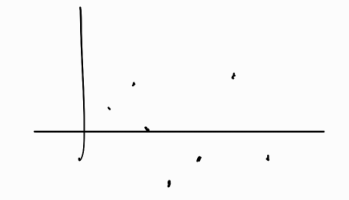
\includegraphics[width=0.7\linewidth]{img/screenshot003}
		\caption{Fucking hell.}
		\label{fig:screenshot003}
	\end{figure}
	We want to think, though, about a continuous space and time process: 
	\begin{figure}[H]
		\centering
		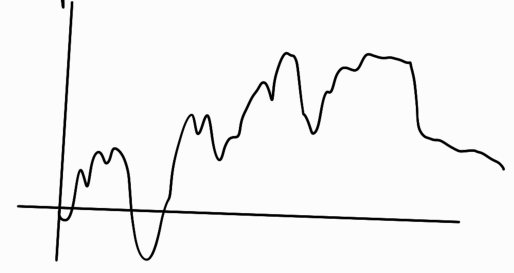
\includegraphics[width=0.7\linewidth]{img/screenshot004}
		\caption{Leaning like my academic career.}
		\label{fig:screenshot004}
	\end{figure}
	How can we define the continuity of the sample paths? and how can we check this property? There are some possible definitions of continuity. To control for their robustness we check whether according to each of these definitions the Poisson process, a discrete process, is correctly classified as non continuous.
	\begin{definition}
		A stochastic process $\{M(t)\}$ is said to be a \emph{counting process} if:
		\begin{enumerate}[i.]
			\item $M(t)>0$;
			\item $M(t)$ is an integer;
			\item $M(t)$ is increasing, meaning that $s\leq t\implies M(s)\leq M(t)$.
		\end{enumerate}
	\end{definition}
	In general, these processes count how many times an event happens.
	\begin{definition}
		A Poisson process is a counting process such that:
		\begin{enumerate}
			\item $N(0)=0$;
			\item for $t_1<t_2<t_3<t_4$ we have
			\begin{equation*}
				N(t_2)-N(t_1)\independent N(t_4)-N(t_3)
			\end{equation*}
			meaning that the increments are independent;
			\item for $\every h>0$ and $t>\tau$ it holds:
			\begin{equation*}
				N(t)-N(\tau)\sim N(t+h)-N(\tau+h)
			\end{equation*}
			meaning that the increments are stationary (the origin start doesn't matter);
			\item we have $$\pr(N(t)=k)=\frac{(\lambda t)^{k}}{k!}e^{-\lambda t}\qquad\text{for } k=0,1,\ldots$$
		\end{enumerate}
	\end{definition}
	\begin{figure}[h]
		\centering
		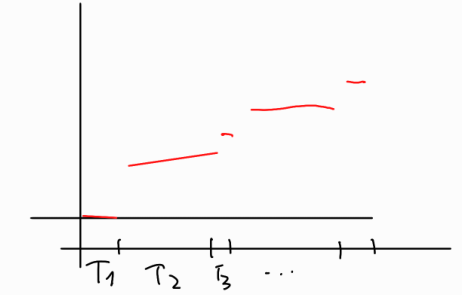
\includegraphics[width=0.7\linewidth]{img/screenshot002}
		\caption{I am very good at drawing straight lines.}
		\label{fig:screenshot002}
	\end{figure}
	
	The inter-arrival times are i.i.d. \rv s distributed as
	\begin{equation*}
		T_i\distexp{\lambda}.
	\end{equation*}
	The continuity of sample paths can be characterized in four different ways:
	\begin{enumerate}
		\item \emph{Continuity in mean squares}: we have this if for $\every t\geq0$ we have
		\begin{equation*}
			\lim_{s\to t}\evs\left[|X(t)-X(s)|^{2}\right]=0.
		\end{equation*}
		So according to this definition, the mean square of the distance goes to 0 if we go near $s$.
		\item \emph{Continuity in probability}: we have this if for $\every t\geq0$ and $\every\varepsilon>0$ we have
		\begin{equation*}
			\lim_{s\to t}\pr(|X(t)-X(s)|>\varepsilon)=0.
		\end{equation*}
		This should be enough for all finite distributions, right?\footnote{First, but not last, question without an answer.}
		\begin{theorem}
			Let $\{X(t)\}$ be a stochastic process such that $\evs[X^{2}(t)]<\infty$ for all $t$. Then it is continuous in mean squares\ifonly{}:
			\begin{enumerate}
				\item $m(t)=\evs[X(t)]$ is continuous;
				\item the covariance function
				\begin{equation*}
					\Gamma(s,t)=\evs[(X(t)-m(t))(X(s)-m(s))]
				\end{equation*}
				is continuous on its diagonal set.
			\end{enumerate}
		\end{theorem}
					\begin{fancyproof}
			Consider the expectation
			\begin{equation*}
				\evs\left[|X(t)-X(s)|^{2}\right]=\evs\left[|X^{2}(s)+X^{2}(t)-2X(t)X(s)|\right]\tag{\faAdjust}\label{boh}
			\end{equation*}
			but
			\begin{equation*}
				\evs\left[X^{2}(s)\right]=\ubracketthin{\evs\left[(X(s)-m(s))^{2}\right]}_{\Gamma(s,s)}+2m(s)\evs\left[X(s)\right]-m^{2}(s)
			\end{equation*}
			and
			\begin{equation*}
				\evs\left[X^{2}(t)\right]=\Gamma(t,t)+2m(t)\evs[X(t)]-m^{2}(t)
			\end{equation*}
			and, moreover,
			\begin{equation*}
				\evs[X(s)X(t)]=\Gamma(s,t)-\cancel{m(t)m(s)}+m(t)\evs[X(s)]+\cancel{m(s)\evs[X(t)]}.
			\end{equation*}
			So \ref{boh} becomes
			\begin{align*}
				\text{\faAdjust}&=\Gamma(s,s)+2m^{2}(s)-m^{2}(s)+\Gamma(t,t)+2m^{2}(t)-m^{2}(t)-2\evs\left[X(s)X(t)\right]\\
				&=\Gamma(s,s)+\Gamma(t,t)-2\Gamma(s,t)+m^{2}(t)+m^{2}(s)-2m(t)m(s)\\
				&=\Gamma(s,s)+\Gamma(t,t)-2\Gamma(s,t)+\left[m(t)-m(s)\right]^{2}.
			\end{align*}
			Hence, if $m(t)$ is continuous and $\Gamma(s,t)$ is continuous for $s=t$ then the process is continuous because we have:
			\begin{itemize}
				\item $[m(t)-m(s)]^{2}\to0$ since it is a continuous function;
				\item $\Gamma(s,s)+\Gamma(t,t)-2\Gamma(s,t)$ that becomes $\Gamma(t,t)+\Gamma(t,t)-2\Gamma(t,t)=0$.
			\end{itemize}
			I'd like to add that dear prof. Sacerdote didn't explain this last little point. Thank you! So now whe have
			\begin{equation*}
				\evs\left[|X(s)-X(t)|^{2}\right]\to0.
			\end{equation*}
			If this holds for $m(t)$ and $\Gamma(t,t)$ then it is continuous in mean squares.
		\end{fancyproof}
		\begin{remark}
			A process continuous in mean \faSquare[regular] (get it?) is continuous in probability (use Chebyshev\footnote{Like use him? As a person? He is dead.}).
		\end{remark}
		Is the Poisson process continuous in mean \faSquare[regular] (and also in probability)? We know that
		\begin{equation*}
			m(t)=\lambda t
		\end{equation*}
		and 
		\begin{align*}
			\Gamma(s,t)&=\evs[(N(t)-m(t))(N(s)-m(s))]\\
			&=\evs[N(t)N(s)]-2m(t)m(s)-m(t)m(s)\\
			&\underset{t>s}{=}\evs[(N(t)-2N(s)+N(s))N(s)]-m(t)m(s)\\
			&=\evs[(N(t)-N(s))N(s)]+\evs\left[N^{2}(s)\right]-m(t)m(s)\\
			&=\ubracketthin{\evs[N(t)-N(s)]}_{
			\lambda(t-s)}\ubracketthin{\evs(N(s))}_{\lambda s}+\evs\left[N^{2}(s)\right]-\ubracketthin{m(t)}_{\lambda t}\ubracketthin{m(s)}_{\lambda s}\\
			&=\lambda^{2}(\cancel{t}-s)s-\cancel{\lambda^{2}ts}+\evs\left[N^{2}(s)\right]\\
			&=-\lambda^{2}s^{2}+\ubracketthin{\var N(s)}_{\lambda s}+\ubracketthin{\left[\evs\left[N(s)\right]\right]^{2}}_{\lambda^{2}s^{2}}\\
			&=\lambda s\qquad\text{if }s<t.
		\end{align*}
	\begin{figure}[h]
		\centering
		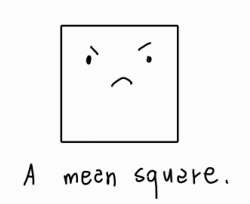
\includegraphics[width=0.3\linewidth]{img/screenshot001}
		\caption{Sei un fallito.}
		\label{fig:screenshot001}
	\end{figure}
	So $\Gamma(s,t)=\lambda\min(s,t)$ is continuous on diagonal and $m(t)=\lambda t$ is also continuous... but this would mean that Poisson processes are continuous! Which they shouldn't be! Do I care? No!
	\item \emph{Almost sure continuity}: we can ask, as a requirement, that
	\begin{equation*}
		\pr\left(\lim_{s\to t}N(s)=N(t)\right)=1.
	\end{equation*}
	Does this finally solve the problem with the Poisson processes? No, because it verifies the almost sure continuity (since it is discontinuous only in a countable number of instances).\\
	It is not enought ot think point by point: we must think \textit{uniformly}.
	\begin{definition}
		A stochastic process $\{X(t)\}$ has \emph{almost sure continuous sample paths} if, with probability 1, $X(t)$ is a continuous function, that is:
		\begin{equation*}
			\pr(X(t)\text{ has continuous samples})=1.
		\end{equation*}
	\end{definition}
	Of course, the case in which you have exceptional points is not a problem since they have measure 0.
	\begin{figure}[h]
		\centering
		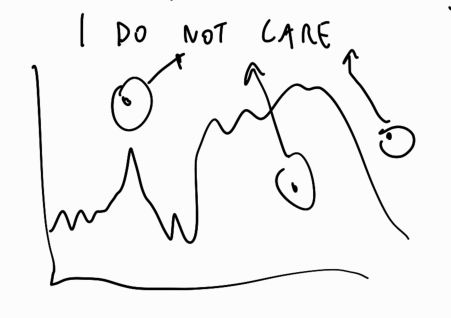
\includegraphics[width=0.4\linewidth]{img/screenshot005}
		\caption{Me neither.}
		\label{fig:screenshot005}
	\end{figure}
	\begin{remark}
		The set
		\begin{equation*}
			\{\omega\in\Omega:t\to B_{t}(\omega)\text{ is continuous}\}
		\end{equation*}
		is not necessarily in the \sa{} generated by the vectors
		\begin{equation*}
			\left(B_{t_{1}}, B_{t_{2}},\ldots,B_{t_{n}}\right)\qquad n\in\N.
		\end{equation*}
	\end{remark}
\end{enumerate}
\section{Definitions of Brownian motion}
\subsection{Historical context}
Imagine a spherical particle with a diameter of $10^{-6}$ m surrounded by $10^{-23}$ (the Avogadro number) molecules with a diameter of $10^{-10}$ m of diameter.
\begin{figure}[h]
	\centering
	\begin{tikzpicture}
		\shade[ball color = gray!40, opacity = 0.4] (0,0) circle (1.2cm);
		\draw (0,0) circle (1.2cm);
		\draw (-1.2,0) arc (180:360:1.2 and 0.6);
		\draw[dashed] (1.2,0) arc (0:180:1.2 and 0.6);
		\fill[fill=black] (0,0) circle (1pt);
		\draw[dashed] (0,0 ) -- node[above]{\tiny$10^{-6}\;m$} (1.2,0);
		\foreach \a in {1,2,...,17}{
			\draw (\a*360/17: 2cm) circle (0.2cm);
			\shade[ball color=Green3,opacity=0.6] (\a*360/17: 2cm) circle (0.2cm);
		}
	\end{tikzpicture}
	\caption{My balls.}
	\label{fig:screenshot006}
\end{figure}
How can we model the behavior of this ball in a mathematical way\footnote{At this point of the lesson Prof. Sacerdote started ranting about Machine Learning (seriously?) being a black box for like 10 minutes.}?\\
In 1828 Robert Brown (fig. \ref{fig:autecre}) observed the chaotic movement of pollen in the water through a microscope and noted:
\begin{itemize}
	\item the motion was composed by translations and rotations;
	\item particles seemed to move independently one from the other;
	\item smallest particles moved more actively;
	\item less viscous fluids determined more activity movement;
	\item the motion never ceased;
	\item the motion was not determined by liquid flows or evaporation;
	\item particles were not animated.
\end{itemize}
In 1905 Einstein gave the correct explanation formulating a model that also proved valid for forecasting: the idea was that the atoms surrounding the particles (the atoms of the fluid) performed a temperature-dependent movement that collided with the particles, changing their direction.\\
\begin{figure}[h]
	\centering
	
\includegraphics[width=0.5\linewidth]{img/screenshot006}
	\caption{Autechre are a IDM duo from Rochdale, England, composed by Robert Brown and Sean Booth.}
	\label{fig:autecre}
\end{figure}
In 1906 the Polish mathematician Smoluchowski independently obtained results similar to Einstein's. Unrelated, but in 1909 Jean Perrin determined the size of atoms.\\
The Einstein approach considers the motion of a particle over a small interval $T$ observed in a time large enough to see at least 2 intervals $t$ independent. Consider, for the sake of simplicity, the one-dimensional case. During $t$ the particle moves of a distance $\Delta$, that is a \rv{} with density $\varphi(\Delta)$ that must be symmetric so $\varphi(\Delta)=\varphi(-\Delta)$. For example, we can imagine $\varphi(\Delta)\sim\mathsf{N}$ with mean 0 (since in this model we do not expect a drift) and small variance. Then we can consider
\begin{equation*}
	\gamma=f(x,t)\qquad\text{as the number of particles per unit of volume.}
\end{equation*}
Einstein proved that $f$ verifies
\begin{equation*}
	\frac{\partial f}{\partial t}=D\frac{\partial^{2}f}{\partial x^{2}}.
\end{equation*}
This was the equation of heat diffusion that was already well known at the time. And so was its solution, which is
\begin{equation*}
	f(x,t)=\frac{1}{\sqrt{4\pi Dt}}e^{-\frac{x^{2}}{4Dt}}.
\end{equation*}
In this case $D$ had a physical meaning: Einstein proved\par
\noindent
\begin{minipage}{0.5\textwidth}
	\begin{equation*}
		D=\frac{1}{\sqrt{6\pi r\eta}}\frac{RT}{N}
	\end{equation*}
\end{minipage}\begin{minipage}{0.5\textwidth}
\begin{itemize}
	\item $\eta$: dynamic viscosity
	\item $r$: dimension of particles
	\item $R$: gas constant (8.3 $\frac{\mathrm{J}}{\mathrm{mol~K}}$)
	\item $T$: absolute temperature
	\item $N$: Avogadro's number
\end{itemize}
\end{minipage}
He could, moreover, calculate the average displacement of a particle
\begin{equation*}
	\lambda_{x}=\sqrt{\overline{x}^{2}}=\sqrt{2Dt}.
\end{equation*}
This means that the displacement (space) is proportional to the square root of time... But what is this story of space and time being related non linearly? This sounded pretty wild for that time.
\begin{figure}[h]
	\centering
	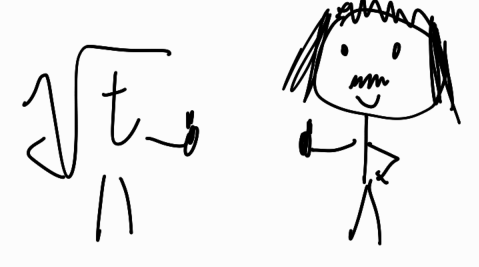
\includegraphics[width=0.5\linewidth]{img/screenshot007}
	\caption{Idk I think I would have probably killed myself.}
	\label{fig:screenshot007}
\end{figure}
\subsection{Random walk model}
We can think that:
\begin{itemize}
	\item each particle starts at $x=0$;
	\item the particle changes position at discrete times
	\begin{equation*}
		k\Delta t \qquad k=1,2,\ldots\qquad\Delta t>0;
	\end{equation*}
	\item the particles move $\Delta X$ units to the right (or to the left) with probability $p=\unmezz$;
	\item $\Delta X$ does not depend on any past position nor on the current position. 
\end{itemize}
\begin{figure}[h]
	\centering
	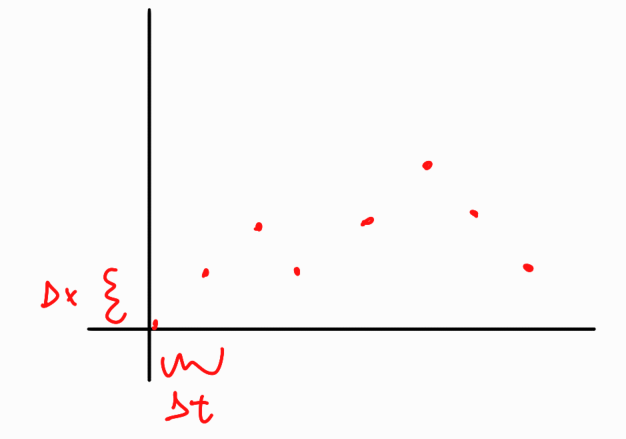
\includegraphics[width=0.5\linewidth]{img/screenshot008}
	\caption{I do not know how to do curly brackets}
	\label{fig:screenshot008}
\end{figure}
When $\Delta X$ and $\Delta t$ go to 0 in an appropriate way, we don't see ``jumps'' anymore but a continuous process:
\begin{figure}[h]
	\centering
	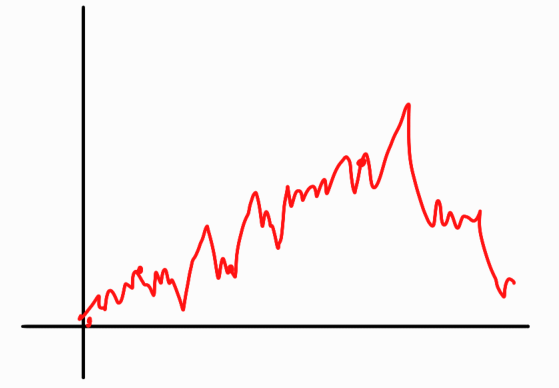
\includegraphics[width=0.5\linewidth]{img/screenshot009}
	\caption{I miss tikzes but they take so much time.}
	\label{fig:screenshot009}
\end{figure}
So we get a continuous process ${\{X_{t}\}}_{t\geq0}$ that is the random position of the time $t$. Introduce the i.i.d. \rv s $\{\varepsilon_{i}\}$ such that $\pr(\varepsilon_{i}=1)=\pr(\varepsilon_{i}=0)=\unmezz$. Then $S_{N}=\sum_{i}^{N}\varepsilon_{i}$ is the number of moves to the right (since moves to the left do not contribute to this count). In the same way, I have $N-S_{N}$ being the number of moves to the left. Now we can write
\begin{align*}
	X_{T}&=\text{positions of particles at }T=N\Delta t\\
	&=S_{N}\Delta X-(N-S_{N})\Delta X\\
	&=(2S_{N}-N)\Delta X\\
	&=\sum_{k=1}^{N}(2\varepsilon_{k}-1)\Delta X.
\end{align*}
\begin{remark}
	For any two times $t=n\Delta t$ and $T=N\Delta t$, $0<t<T$, we can write:
	\begin{align*}
		X_{T}&=(X_{T}-X_{t})+(X_{t}-X_{0})\\
		&=\sum_{k=n+1}^{N}(2\varepsilon_{k}-1)\Delta X+\sum_{k=1}^{n}(2\varepsilon_{k}-1)\Delta X.
	\end{align*}
		\begin{center}
			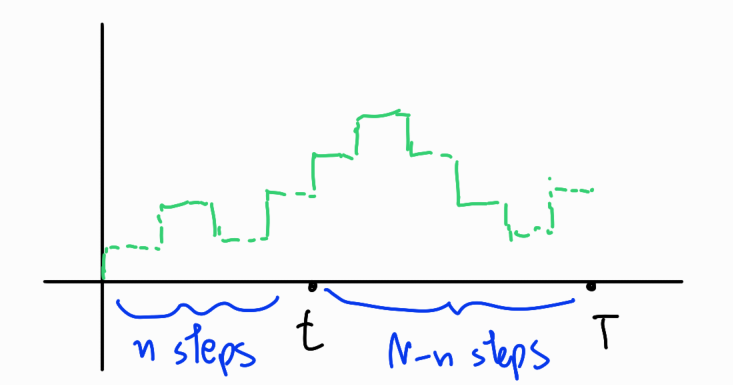
\includegraphics[width=0.5\linewidth]{img/screenshot010}
		\end{center}
	But these quantities involve different $\varepsilon$, so they are independent:
	\begin{equation*}
		X_{T}-X_{t}\independent X_{t}-X_{0}\qquad\text{(independent increments.)}
	\end{equation*}
	But we know that 
	\begin{equation*}
		\evs\varepsilon_{i}=\unmezz\qquad\mathrm{and}\qquad\var\varepsilon_{i}=\frac{1}{4}
	\end{equation*}
	so
	\begin{align*}
		\var X_{T}&=\var\left[\sum^{}{N}_{k}(2\varepsilon_{k}-1)\Delta X\right]\\
		&\overset{i.i.d.}{=}\sum^{N}_{k}\left(\Delta X\right)^{2}\var(2\varepsilon_{k}-1)\\
		&=\sum_{k}^{N}(\Delta X)^{2}\cancel{4}\ubracketthin{\cancel{\var \varepsilon_{k}}}_{\frac{1}{4}}\\
		&=N(\Delta X)^{2}.
	\end{align*}
	But $N=\frac{T}{\Delta t}$ so 
	\begin{equation*}
		N(\Delta X)^{2}=\frac{(\Delta X)^{2}}{\Delta t}T=\sigma^{2}T.
	\end{equation*}
\end{remark}
So this should be the variance of our random walk. If we take the limit for $x$ and $t$ and do nost take into account that space and time decrease in different ways we get a process that has mean 0 and variance 0... but that is a process that is 0 almost surely! So we get the idea that time and space must decrease at different speeds. We also said that the increments must be stationary, but that has its implications.
\begin{remark}
	We know that $\var 2S_{N}=N$, but
	\begin{align*}
		X_{T}&=(2S_{N}-\ubracketthin{N}_{\mathclap{\evs 2 S_{N}}})\Delta X\\
		&=\frac{2 S_{N}-\evs 2 S_{N}}{\mathcolor{Green4}{\sqrt{N}}}\mathcolor{Green4}{\sqrt{N}}\Delta X\\
		&=\frac{2S_{N}-\evs 2 S_{N}}{\sqrt{\var(2S_{N})}}\ubracketthin{\sqrt{N}}_{\sqrt{\frac{T}{\delta t}}}\ubracketthin{\Delta X}_{{\sigma\sqrt{\Delta t}}}\\
		&=\frac{2S_{N}-\evs 2 S_{N}}{\ubracketthin{\sqrt{\var(2S_{N})}}_{\claptext{This gets to $Z\distnorm{0,1}$ as $N\to\infty$}}}\sigma\sqrt{T}.
	\end{align*}
	So we get that this quantity gets to $Z\sigma\sqrt{t}$ and it is true for each $t$:
	\begin{equation*}
		X_{t}\distnorm{0,t\sigma^{2}}.
	\end{equation*}
\end{remark}
\subsection{Definitions}
\begin{definition}
	\emph{Definition of Brownian Motion} (1923, by Norbert Wiener).\\
	A stochastic process $B={\{B_{t}\}}_{t\geq 0}$ defined on a probability space $(\Omega,\F,\pr)$ and taking values in $\R$ is called \emph{standard Brownian motion} (or \emph{standard Wiener process}) if:
	\begin{enumerate}
		\item the function $t\mapsto B_{t}$ is \ul{continuous} from $\R_{+}$ to $\R$ and $B_{0}=0$ (both almost surely);
		\item $B$ has \ul{stationary increments} (they don't depend on the origin):
		\begin{equation*}
			B_{t}-B_{s}\sim B_{t+h}-B_{s+h}\qquad\evs 0<s<t\qquad\every f>0;
		\end{equation*}
		\item $B$ has \ul{independent} increments, i.e. for any $0\leq t_{0}\leq t_{1}<\leq t_{2}\leq\ldots\leq t_{n}$ and $n\geq 1$ we have:
		\begin{equation*}
			B_{t_1}-B_{t_0}, B_{t_2}-B_{t_1},\ldots,B_{t_{n}}-B_{t_{n-1}}\qquad\text{independent};
		\end{equation*}
		\item $B_{t}\distnorm{0,t}$ for $\every t\geq 0$.
	\end{enumerate}
\end{definition}
\begin{definition}
	\emph{General Brownian motion} (Brownian motion with drift).\\
	\begin{equation*}
		X_{t}=\ubracketthin{\mu}_{\claptext{drift}} t+\ubracketthin{\sigma}_{D=\frac{\sigma^{2}}{2}} B_{t}.
	\end{equation*}
	This process verifies properties 1, 2, 3 and
	\begin{equation*}
		X_{t}\distnorm{\mu t,\sigma^{2}t}.
	\end{equation*}
\end{definition}
We can now proceed to define the $d$-dimensional \bwm{}:
\begin{definition}
	A $d$-dimensional \bwm, $B={\{B_{t}\}}_{t\geq 0}$ is a stochastic process indexed by $[0,\infty)$ taking values on $\R^{d}$ such that:
	\begin{enumerate}
		\item $B_{0}(\omega)=0$ \as{} $\every\omega\in\Omega$;
		\item $B_{t_{n}}-B_{t_{n-1}},\ldots,B_{t_{1}}-B_{t_{0}}$ are independent fo $\every n>1,\;0\leq t_{1},t_{2}<\ldots<t_{n}<\infty$ (\emph{independent increments});
		\item $B_{t}-B_{s}\sim B_{t+h}-B_{s+h}$ for $\every h>0$, $\every 0\leq s<t<\infty$ (\emph{stationary increments});
		\item $B_{t}-B_{s}\distnorm{0,t-s}^{\otimes d}$ with 
		\begin{equation*}
			\mathsf{N}(0,t)\dx =\frac{\dx}{\sqrt{2\pi t}}\exp\left\{-\frac{x^{2}}{2t}\right\}
		\end{equation*} (\emph{Gaussian increments});
		\item $t\mapsto B_{t}(\omega)$ is continuous for all $\omega$ (\emph{continuity of sample paths}).
	\end{enumerate}
\end{definition}
Remember that 
\begin{equation*}
	1,2,3,5\implies 4\qquad\text{and}\qquad1,2,3,4\implies 5
\end{equation*}
for almost all $\omega$. A standard \bwm{} on $\R^{d}$ is obtained by setting
\begin{equation*}
	B=(B^{1},B^{2},\ldots,B^{d})
\end{equation*}
where $B^{1},B^{2},\ldots$ are independent \bwm{} on $\R$ called \ul{coordinate processes}.
\begin{definition}
	The continuous process $W$ is called \emph{Wiener process} with respect to $\mathscr{A}$ if it is adapted to $\mathscr{A}$ (check that adaptness is included in the above definitions!) and 
	\begin{equation*}
		\evs_{s}f[W_{s+t}-W_{s}]=\int_{\R}\dx\left[\frac{e^{-\frac{x^{2}}{2t}}}{\sqrt{2\pi t}}f(x)\right]\qquad\text{for $f$ positive Borel function and }\every s,t\in\R_{+}.
	\end{equation*}
\end{definition}
\begin{exercise}
	Prove that the second definition of \bwm{} implies the first for $d=1$.
\end{exercise}
But with these properties there is the risk that no such object exists! For example, if we add differentiability to our list of requests then no object satisfies such properties. So we need to ask two questions:
\begin{itemize}
	\item Does \bwm{} exists?
	\item Is it unique?
\end{itemize}
Wiener worked on the difference space, that is the space of the increments of the process, and introduced a Fourier series representation:
\begin{equation*}
	W_t=\xi_{0}t+\sqrt{2}\sum_{n=1}^{\infty}\xi_{n}\frac{\sin(n\pi t)}{\pi n}\qquad0\leq t\leq 1
\end{equation*}
where $\{\xi_{i}\}$ are i.i.d. \rv s $\xi_{i}\distnorm{0,1}$, so this object is a Fourier series for which the coefficients are \rv s. Thinking about difference equations makes our life a bit easier, since different times have different $\xi_{i}$ but these are independent so also the increment between times are independent.
\section*{Exercises}
\label{sec:exer1}
\addcontentsline{toc}{section}{\nameref{sec:exer1}}
\begin{exercise}
	Consider a continuous process $W={(W_{t})}_{t\geq0}$ adapted to $\F$ and let 
	\begin{equation*}
		\evs_{s}\left[f(W_{t+s}-W_{s})\right]=\int_{\R}\dx\frac{1}{\sqrt{2\pi t}}\exp\left\{-\frac{x^{2}}{2t}\right\}f(x)
	\end{equation*}
	for all $s$ and $t$ in $\R_{+}$ and all positive Borel functions $f$ on $\R$. Show that $W$ is a standard $BM$.
\end{exercise}
	We need to check the five properties:
\begin{enumerate}
	\item $B_{0}(\omega)=0$ \as{} $\every\omega\in\Omega$. We know that the increment has the same distribution as a Gaussian \rv{} distributed as $\mathsf{N}(0,t)$. This means that as $t\to0$ the distribution collapses towards a Dirac measure centered at 0:
	\begin{equation*}
		W_{t}-W_{0}\xrightarrow{t\to0}0\qquad\text{in distribution}
	\end{equation*}
	but since $W_{t}$ is continuous in $t$ then we know that 
	\begin{equation*}
		W_{0}=\lim_{t\to0}W_{t}.
	\end{equation*}
	So it must be the case that 
	\begin{equation*}
		W_{0}=0.
	\end{equation*}
	Technically, convergence in distribution + continuity should imply a.s. convergence because there are no jumps in the distribution!\hspace*{\fill}\faCheckCircle
	\item $B_{t_{n}}-B_{t_{n-1}},\ldots,B_{t_{1}}-B_{t_{0}}$ are independent for $\every n>1,\;0\leq t_{1},t_{2}<\ldots<t_{n}<\infty$ (\emph{independent increments}). The increment $W_{s+t}-W_{s}$ over the interval $(s,s+t)$ is independent of the past $\F_{s}$ (and its distribution is $\mathsf{N}(0,t)$).\hspace*{\fill}\faCheckCircle
	\begin{insult}
		I had to search \cinlar's horrid book for this!
	\end{insult}
	\item $B_{t}-B_{s}\sim B_{t+h}-B_{s+h}$ for $\every h>0$, $\every 0\leq s<t<\infty$ (\emph{stationary increments}). This works because the distribution of the interval does not depend on $s$ but only on $t$.\hspace*{\fill}\faCheckCircle
	\item $B_{t}-B_{s}\distnorm{0,t-s}^{\otimes d}$ with 
	\begin{equation*}
		\mathsf{N}(0,t)\dx =\frac{\dx}{\sqrt{2\pi t}}\exp\left\{-\frac{x^{2}}{2t}\right\}
	\end{equation*} (\emph{Gaussian increments}). This follows by definition, I guess.\hspace*{\fill}\faCheckCircle
	\item $t\mapsto B_{t}(\omega)$ is continuous for all $\omega$ (\emph{continuity of sample paths}).\hspace*{\fill}\faCheckCircle
\end{enumerate}
\begin{exercise}
	Show that there exist a random vector $(U,V)$ such that $U$ and $V$ are one dimensional Gaussian \rv s but $(U,V)$ is not Gaussian. Hint: try 
	\begin{equation*}
		f(u,v)=g(u)g(v)(1-\sin u\sin v)
	\end{equation*}
	with 
	\begin{equation*}
		g(u)=\frac{\exp\left\{-\frac{u^{2}}{2}\right\}}{\sqrt{2\pi}}.
	\end{equation*}
\end{exercise}
We can compute the marginal densities:
\begin{align*}
	f_{V}(v)&=\int_{-\infty}^{\infty}g(u)g(v)(1-\sin u\sin v)\du\\
	&=g(v)\int_{-\infty}^{\infty}g(u)(1-\sin u\sin v)\du\\
	&=g(v)\biggl[\ubracketthin{\int_{-\infty}^{\infty} g(u)\du}_{1}-\sin v\ubracketthin{\int_{-\infty}^{\infty}g(u)\sin u\du}_{\claptext{odd function, so the integral is 0}}\biggr]\\
	&=g(v).
\end{align*}
So the marginal density is Gaussian! Do the same with the other marginal density to obtain the same shit.
\begin{exercise}
	Consider a random walk with independent steps ${\{Z_{i}\}}_{i=1,\ldots}$ each having the distribution:
	\begin{equation*}
		\pr(Z=\Delta)=p,\pr(Z=-\Delta)=1-p=q
	\end{equation*}
	with $p>0$. Suppose that these steps of size $\Delta$ take place at small time interval of length $\tau$. We are interested in the limit process when $\Delta$ and $\tau$ approach zero.
	\begin{enumerate}
		\item Determine the moment generating function $\ev{\exp\left\{-\vartheta Z\right\}}$ of $Z$.
		\item Observe that at time $t$ there are $n=\lfloor\frac{1}{\tau}\rfloor\sim\frac{1}{\tau}$ steps and that the total displacement at time $t$, $X(t)$, is the sum of $n$ independent \rv s. Determine $\ev{\exp\left\{-\vartheta X(t)\right\}}$.
		\item Determine the mean and variance of $X(t)$.
		\item Propose a suitable way to let $\Delta\to0$ and $\tau\to0$ to obtain a meaningful result for the continuous space and time limit process. Hint: we want to obtain
		\begin{equation*}
			(p-q)\frac{\Delta}{\tau}\to\mu,\qquad4pq\Delta^{2}\to\sigma^{2}.
		\end{equation*}
		\item Is the obtained process a \bwm{} with drift?
	\end{enumerate}
\end{exercise}
So we know that the m.g.f of one step (and all steps are mutually independent) is
\begin{equation*}
	\ev{e^{-\vartheta Z}}=pe^{-\vartheta Z}+(1-p)e^{-\vartheta Z}.\tag{\faBusinessTime}\label{biz}
\end{equation*}
Observe that in time $t$ there will be $n=\sfrac{t}{\tau}$ steps. We know that the mean and variance of the total displacement $X(t)$ are
\begin{equation*}
	\begin{array}{c}
		\ev{X(t)}=n\cdot\ev{Z}=\frac{t}{\tau}(p-q)\Delta\\
		\var(X(t))=\ev{Z^{2}}-(\ev{Z})^{2}=\frac{t}{\tau}4pq\Delta^{2}.
	\end{array}
\end{equation*}
The computations should be right... We want to let $\Delta\to0$ and $\tau\to0$ so that we obtain a continuous result by scaling the step size and the time step to zero. Suppose we require the limiting process to have mean $\mu$ and variance $\sigma^2$ in unit time, which means requiring $\Delta$ and $\tau$ to tend to zero in such a way that 
\begin{equation*}
	(p-q)\frac{\Delta}{\tau}\to\mu,\qquad4pq\Delta^{2}\to\sigma^{2}
\end{equation*}
That is, the expected displacement per step must converge to a finite value. This is like forcing the limit to make sense, otherwise just letting $\Delta\to0$ and $\tau\to0$ we obtain 0 mean and 0 variance. Which means 0 bitches. You want that? I don't. The main idea is that $\Delta$ must be go to zero slower than $\tau$: by setting $\Delta=\sigma\sqrt{\tau}$ we obtain that the displacement $\Delta$ is of a considerably larger order of magnitude than the small time interval $\tau$ in which it occurs. So our request will be satisfied with
\begin{align*}
	\Delta&=\sigma\sqrt{\tau}\\
	p&=\unmezz\left(1+\frac{\mu\sqrt{\tau}}{\sigma}\right)\\
	q&=\unmezz\left(1-\frac{\mu\sqrt{\tau}}{\sigma}\right).
\end{align*}
We can now substitute these mfs in \ref{biz} and get
\begin{equation*}
	\ev{e^{-\vartheta X(t)}}=\left[\unmezz\left(1+\frac{\mu\sqrt{\tau}}{\sigma}\right)e^{-\vartheta\sigma\sqrt{\tau}}+\unmezz\left(1-\frac{\mu\sqrt{\tau}}{\sigma}\right)e^{\vartheta\sigma\sqrt{\tau}}\right]^{\frac{t}{\tau}}.
\end{equation*}
We already know that:
\[
\ev{X(t)} = \frac{t}{\tau} (p - q) \Delta = \frac{t}{\tau} \left( \frac{\mu \sqrt{\tau}}{\sigma} \right) \sigma \sqrt{\tau} = \mu t.
\]
This shows that the expected displacement of the random walk at time \(t\) converges to a linear function of \(t\), with slope \(\mu\), as required. This means that the limiting process has drift \(\mu\).
Next, for the variance:
\[
\var(X(t)) = \frac{t}{\tau} \cdot 4pq \Delta^2.
\]
Substituting \(\Delta = \sigma \sqrt{\tau}\), we get:
\[
\var(X(t)) = \frac{t}{\tau} \cdot 4pq (\sigma \sqrt{\tau})^2 = \frac{t}{\tau} \cdot 4pq \sigma^2 \tau = 4pq \sigma^2 t.
\]
Now, substituting \(p = \frac{1}{2} \left( 1 + \frac{\mu \sqrt{\tau}}{\sigma} \right)\) and \(q = \frac{1}{2} \left( 1 - \frac{\mu \sqrt{\tau}}{\sigma} \right)\), we get:
\[
4pq = 4 \cdot \frac{1}{2} \left( 1 + \frac{\mu \sqrt{\tau}}{\sigma} \right) \cdot \frac{1}{2} \left( 1 - \frac{\mu \sqrt{\tau}}{\sigma} \right) = 1 - \left( \frac{\mu \sqrt{\tau}}{\sigma} \right)^2.
\]
Thus, we have:
\[
\var(X(t)) = \left( 1 - \left( \frac{\mu \sqrt{\tau}}{\sigma} \right)^2 \right) \sigma^2 t.
\]
Taking the limit as \(\tau \to 0\), we see that the term involving \(\mu\) vanishes and the variance becomes:
\[
\var(X(t)) = \sigma^2 t,
\]
which is precisely the variance of a Brownian motion with variance \(\sigma^2\).
\begin{exercise}
	Ignoring the requested continuity of sample paths of the \bwm{} show that the \bwm{} is continuous in mean square.
\end{exercise}
The process is continuous in mean square if the expectation of the squared difference between $B(t)$ and $B(s)$ goes to 0 as $t\to s$:
\begin{equation*}
	\lim_{s\to t}\ev{\left(B(t)-B(s)\right)^{2}}=0.
\end{equation*}
We know that $\ev{B(t)}=0$, that is continuous because the mean is trivially constant over time (duh). The covariance function is, for $s\leq t$,
\begin{align*}
	\Gamma(s,t)&=\cov(B(s),B(t))\\
	&=\ev{B(s)B(t)}-\ubracketthin{\ev{B(s)}}_{0}\ubracketthin{\ev{B(t)}}_{0}\\
	&=\ev{B(s)B(t)}\\
	&=\ev{B(s)(\mathcolor{SpringGreen4}{B(s)}+B(t)-\mathcolor{SpringGreen4}{B(s)})}\\
	&=\ev{B(s)^{2}}+\evs[B(s)(\ubracketthin{B(t)-\mathcolor{SpringGreen4}{B(s)}}_{\claptext{$\independent$ of $B(s)$}})]\\
	&=\ev{B(s)^{2}}+\ubracketthin{\evs[B(s)]}_{=0}\evs[(B(t)-\mathcolor{SpringGreen4}{B(s)})]\\
	&=\ev{B(s)^{2}}\\
	&=s=\min\{s,t\}.
\end{align*}
\begin{insult}
	It would have been useful to know about this little property during lesson...
\end{insult}
We know that $\min\{s,t\}\big|_{s=t}=t$ so our limit is:
\begin{align*}
	\lim_{s\to t}\ev{\left(B(t)-B(s)\right)^{2}}&=\lim_{s\to t}\left(\ev{B(t)^{2}}-2\ubracketthin{\ev{B(t)B(s)}}_{\Gamma(s,t)}+\ev{B(s)^{2}}\right)\\
	&=\lim_{s\to t}\left(t-2t+t\right)=0.
\end{align*}
-
\section{\bwm{} as a Gaussian processes}
\subsection{Properties of Gaussian Processes}
\begin{definition}
	A \emph{Gaussian process} is defined as a process $\Gamma$ with
	\begin{equation*}
		\begin{array}{rclr}
			\frac{\dif}{\dif \lambda}\evs\left[e^{i\lambda\Gamma}\right]\Big|_{\lambda=0}&=&im&m=\evs[\Gamma]\\
			\frac{\dif^{2}}{\dif\lambda^{2}}\evs\left[e^{i\lambda\Gamma}\right]\Big|_{\lambda 0}&=&-\evs\left[\Gamma^{2}\right].&
		\end{array}
	\end{equation*}
\end{definition}
\begin{definition}
	A random vector
	\begin{equation*}
		\Gamma=(\Gamma_{1},\Gamma_{2},\ldots,\Gamma_{n})\in\R^{n}
	\end{equation*}
	is Gaussian if the scalar product 
	\begin{equation*}
		\langle\lambda,\Gamma\rangle\qquad\every\lambda\in\R^{n}
	\end{equation*}
	is a one-dimensional Gaussian \rv{} with:
	\begin{equation*}
		\evs\left[e^{i\langle\lambda,\Gamma\rangle}\right]=e^{i\evs\left[\langle\lambda,\Gamma\rangle\right]-\unmezz\var\left(\langle\lambda,\Gamma\rangle\right)}.
	\end{equation*}
\end{definition}
So setting 
\begin{equation*}
	\begin{array}{cc}
		m=(m_{1},\ldots,m_{n})\in\R^{n}&m_{j}=\evs[\Gamma_{j}]\\
		&\\
		\Sigma={(\sigma_{jk})}_{jk}\in\R^{n\times m}&\begin{array}{rl}
			\sigma_{jk}&=\evs\left[(\Gamma_{j}-m_{j})(\Gamma_{k}-m_{k})\right]\\
			&=\cov(\Gamma_{j},\Gamma_{k})\\
			&=\Sigma_{j,k}
		\end{array}
	\end{array}
\end{equation*}
So that 
\begin{equation*}
	\evs\left[e^{i\langle\lambda,\Gamma\rangle}\right]=e^{i\langle\lambda,m\rangle-\unmezz	\langle\lambda,\Sigma\lambda\rangle}.
\end{equation*}
The basic idea is that I can linearly transform a random vector and it still is a Gaussian \rv. Fourier transform always exists even for limits, while it is not so easy for distributions. What happens if we apply to a Gaussian vector a matrix that turns it into a subspace? Do I care? Not much! But imagine the classic Gaussian \rv:
\begin{equation*}
	f(x)=\frac{1}{\sqrt{2\pi \sigma^{2}}}\exp\left\{-\frac{x^{2}}{2\sigma^{2}}\right\}.
\end{equation*}
If I take $\sigma\to0$ then the density degenerates into a Dirac measure.
\begin{figure}[h]
	\centering
	\begin{tikzpicture}
	\begin{axis}[every axis plot post/.append style={
			mark=none,domain=-2:2,samples=20,smooth}, % All plots: from -2:2, 50 samples, smooth, no marks
		axis x line*=bottom, % no box around the plot, only x and y axis
		axis y line*=left,
		axis lines=center, % the * suppresses the arrow tips
		enlargelimits] % extend the axes a bit to the right and top
		\addplot[SpringGreen3] {gauss(0,0.5)} node[pos=0.75,anchor=south west]{$\sigma_{2}$};
		\addplot[Turquoise4] {gauss(0,0.75)} node[pos=0.9,anchor=south west]{$\sigma_{1}$};
		\addplot[OliveDrab4] {gauss(0,0.2)} node[pos=0.6,anchor=south west]{$\sigma_{3}$};
	\end{axis}
	\end{tikzpicture}
	\label{fig:gaugau}
	\caption{It will become a dirac measure... but that is not a fucking density.}
\end{figure}
This is still technically a measure because it integrates to 1, but it is not a density anymore since we lose dimensionality on $\R$ which is\footnote{As I learn now.} the meaning of becoming a subspace! But now consider the characteristic function
\begin{equation*}
	\evs\left[e^{i\lambda x}\right]=e^{-1\lambda\frac{\sigma^{2}}{2}}\xrightarrow{\sigma\to0}\ubracketthin{1}_{\claptext{characteristic function of degenerate \rv s.}}.
\end{equation*}
The main point about this is that we could still take a limit. If we were working with density we couldn't have done that.\par
The alternative definition for Gaussian processes are:
\begin{definition}
	A vector valued \rv{} $X$ has $n$-dimensional standard Gaussian distribution if its $n$ coordinates are standard Gaussian in $\R^{1}$ and are independent.
\end{definition} 
\begin{definition}
	A vector valued \rv{} $Y:\Omega\to\R^{n}$ is Gaussian if there exists a vector valued $X$ having $n$-dimensional standard Gaussian distribution and $m\times n$ matrix $A$ and a $m$-dimensional vector $b$ such that
	\begin{equation*}
		Y=AX+b\qquad\text{and }AA^{\trsp}=\Sigma.
	\end{equation*}
\end{definition}
In this case $Y$ us a linear transformation of the Gaussian vector and $A$ projects $X$ in a $m$-dimensional subspace. This is the same procedure we do with Principal Component Analysis, where we diagonalize a matrix and other passages I don't remember and I don't care about.
There are some properties:
\begin{proposition}
	\begin{itemize}
		\item Let $X\distnorm{0,\Sigma_{n}}$. The distribution of $\left[X_{k+1,\ldots,k+n}\right]$ conditioned to $\left[X_{1}=x_{1},\ldots,X_{k}=x_{k}\right]$ is \begin{equation*}
		W(0,\Sigma_{2|1})
		\end{equation*}
		where 
		\begin{equation*}
			\Sigma_{2|1}=\Sigma_{22}-\Sigma_{21}\Sigma_{11}^{-1}\Sigma_{12}
		\end{equation*}
		and 
		\begin{equation*}
			\Sigma=\begin{bmatrix}
				\Sigma_{11}&\Sigma_{12}\\
				\Sigma_{21}&\Sigma_{22}
			\end{bmatrix}.
		\end{equation*}
		Note that the sub-matrices that $\Sigma$ is made of have lower dimensionality.
		\item If $Y=\ubracketthin{a}_{\in\R^{m}}+\ubracketthin{B}_{\in\R^{n}\times\R^{m}}X$ is an affine transformation of $X\distnorm{\mu,\varepsilon}$ then $$Y\distnorm{a+B\mu, B\Sigma B^{\trsp}}.$$
		This is like working with the affine transformation.
	\end{itemize}
\end{proposition}
What about another definition? I think we need it
\begin{definition}
	A Gaussian process is a stochastic process such that for every $t_{1},\ldots,t_{k}$ in the index set $\T$ and each $k>1$ we have that
	\begin{equation*}
		\left(X_{t_{1}},\ldots,X_{t_{k}}\right)=X_{t_{1},\ldots,t_{k}}
	\end{equation*}
	is a multivariate Gaussian random vector (possibly degenerate).
\end{definition}
Now we have defined a class of processes:
\begin{figure}[H]
	\centering
	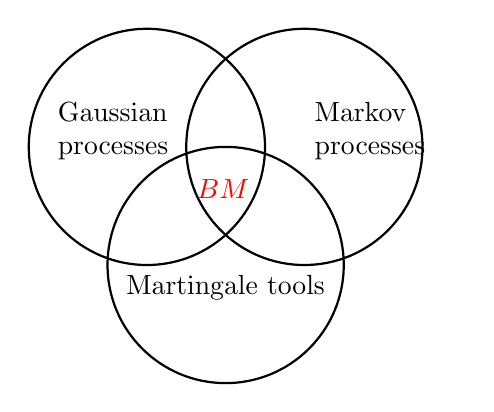
\begin{tikzpicture}
		\draw[thick] (0,0) circle (1.5cm) node[anchor=east,text width=2cm,xshift=1cm,yshift=0.2cm] {Gaussian processes}
		(2,0) circle (1.5cm) node[anchor=west, text width=1.8cm,yshift=0.2cm] {Markov processes} (1,-1.5) circle (1.5cm) node[anchor=north] {Martingale tools};
		\node[anchor=south,yshift=-2.3cm,xshift=-0.3cm,red] at (current bounding box.north) {$BM$};
	\end{tikzpicture}
	\caption{Balls.}
\end{figure}
There is another class: the Levy processes: they have independent and stationary increment (so they are Markov processes) but unlike \bwm{} we don't require continuity on the sample path, but just \ul{continuity on the right of sample paths} and \ul{admit left limit}.
\begin{definition}
	We call \emph{marginal distribution} of $\{B_{t}\}$ the laws of the finite dimension vectors
	\begin{equation*}
		\Gamma_{n}=\left(B_{t_{1}},B_{t_{2}},\ldots,B_{t_{n}}\right)^{\trsp}\qquad 0\leq t_{1}<t_{2}<\ldots<t_{n}<\infty,\quad\every n>0
	\end{equation*}
\end{definition}
There are properties about the increments
\begin{equation*}
	(B_{t_{1}}-B_{t_{0}},B_{t_{2}}-B_{t_{1}},\ldots,B_{t_{n}}-B_{t_{n-1}})
\end{equation*}
but, anyway, for the \bwm{} to be gaussian all $\Gamma_{n}$ must be gaussian. 
\subsection{Gaussianity of \bwm}
\begin{proposition}
	Let $B={\{B_{t}\}}_{t\geq 0}$ be a standard BM in $[0,\infty)$. Let $s,t$ be given and fixed. The covariance will be 
	\begin{equation*}
		\evs\left[B_{t}B_{s}\right]=s\wedge t.
	\end{equation*}
\end{proposition}
\begin{fancyproof}
	Assume, without loss of generality, that $s<t$. Then
	\begin{align*}
		\evs\left[B_{t}B_{s}\right]&=\evs\left[(B_{t}-B_{s}+B_{s})B_{s}\right]\\
		&=\ubracketthin{\evs\left[(B_{t}-B_{s})B_{s}\right]}_{\claptext{independent incrememnts}}+\ubracketthin{\evs[B^{2}_{s}]}_{\var(B_{s})=s}\\
		&=\evs[B_{t}-B_{s}]\ubracketthin{\evs[B_{s}]}_{=0}+s=s.
	\end{align*}
	But, similarly, if $s>t$ then $\evs[B_{t}B_{s}]=t$.
\end{fancyproof}
\begin{remark}
	For every 0$\leq t_{1}<\ldots<t_{n}$ and $n\geq 1$, we have:
	\begin{equation*}
		\begin{array}{l}
			B_{t}\distnorm{0,t}\\
			B_{t_{2}}-B_{t_{1}}\distnorm{0,t_{2}-t_{1}}\\
			\vdots\\
			B_{t_{n}}-B_{t_{n-1}}\distnorm{0, t_{n}-t_{n-1}}.
		\end{array}
	\end{equation*}
	This implies that 
	\begin{equation*}
		\left(B_{t_{1}},\ldots, B_{t_{n}}\right)^{\trsp}\distnorm{\left[\begin{smallmatrix}
				0\\0\\ \vdots\\0\\
		\end{smallmatrix}\right],[t_{i}\wedge t_{j}]^{n}_{i,j=1,\ldots n}}
	\end{equation*}
	which is a $n$-dimensional normal distribution.
\end{remark}
\begin{fancyproof}
	Consider a vector
	\begin{equation*}
		\Delta=\begin{bmatrix}
			B_{t_{1}}-\overbracket{B_{t_{0}}}^{=0}\\
			\vdots\\
			B_{t_{n}}-B_{t_{0}}
		\end{bmatrix}
	\end{equation*}
	and
	\begin{equation*}
		B_{t_{k}}-B_{t_{0}}=\sum^{k}\left(B_{t_{j}}-B_{t_{j-1}}\right).
	\end{equation*}
	Let $M$ be a matrix $n\times n$. We now have the increment but we want a single component. When we want to prove that a vector is Gaussian we usually find a linear transformation that generates another Gaussian.
	\begin{equation*}
		M=\begin{bmatrix}
			1&0&0&\cdots&\cdots&0\\
			1&1&0&\cdots&\cdots&0\\
			1&1&1&&&\vdots\\
			\vdots&\vdots&&1&&\vdots\\
			\vdots&\vdots&&&\ddots&0\\
			1&1&&\cdots&1&1
		\end{bmatrix}.
	\end{equation*}
	Consider $M\Delta=\Gamma$. We have a linear transformation of a Gaussian vector $\Delta$, that is therefore still Gaussian But we notice that $\Gamma$ reconstructs the values of the BM relative to $B_{t_{0}}$. Hence the BMs (that have a finite dimensional distribution) are Gaussian. But if all finite dimensional distributions of the process are Gaussian, then the BM is Gaussian.
\end{fancyproof}
But this means that we can compute the covariance matrix as a simple transformation of the covariance matrix of the original process
\begin{equation*}
	C=M\Sigma M^{\trsp}
\end{equation*}
with $\Sigma$ being the covariance matrix of $\Delta$
\begin{equation*}
	\Sigma=\begin{bmatrix}
		t_{1}-t_{0}&0&\cdots&0\\
		0&t_{2}-t_{1}&&&\vdots\\
		\vdots&&\ddots&0\\
		0&\cdots&0&t_{n}-t_{n-11}
	\end{bmatrix}
\end{equation*}
and
\begin{align*}
	C&=   \ubracketthin{ \left[
	\begin{array}{cccc}
		1                                    \\
		1& 1              & \text{\huge0}\\
		\vdots&               & 1                \\
		1&             \cdots    &   & \ddots
	\end{array}
	\right]}_{M}\ubracketthin{\left[
	\begin{array}{cccc}
		t_{1}-t_{0}                                    \\
		& t_{2}-t_{1}              & \smash{\text{\huge0}}\\
		&\smash{\text{\huge0}}               & \ddots                \\
		&               &   & t_{n}-t_{n-1}
	\end{array}
	\right]}_{\Sigma}\ubracketthin{\left[
	\begin{array}{cccc}
		1                 &1&\cdots        &1           \\
		& 1              & &\vdots\\
		\text{\huge0}&               & 1                \\
		&              &   & \ddots
	\end{array}
	\right]}_{M^{\trsp}}\\
	&=\begin{bmatrix}
		t_{1}&t_{1}&\cdots&t_1\\
		t_{1}&t_{2}&\cdots&t_{2}\\
		\vdots&&&\vdots\\
		t_{1}&t_{2}&\cdots&t_{n}
	\end{bmatrix}={\left[t_{i}\wedge t_{j}\right]}_{n\times n}.
\end{align*}
\begin{remark}
	The vector $\Gamma=\left(B_{1},\ldots,B_{t_{n}}\right)^{\trsp}$ admits a probability density function\footnotemark
	\begin{align*}
		\pr(\Gamma\in\dx)&=\frac{\dx}{(2\pi)^{\frac{n}{2}}\sqrt{\mathsf{det~}C}}\\
		&=\frac{1}{(2\pi)^{\frac{n}{2}}}\sqrt{\prod_{j=1}^{n}(t_{j}-t_{j-1})}\exp\left\{-\unmezz\sum_{j=1}^{n}\frac{(x_{j}-x_{j-1})^{2}}{t_{j}-t_{j-1}}\right\}.
	\end{align*}
	We can see how this has independent components since the exponential depends only by $x_{j}-x_{j-1}$ and all the terms are separated by the summation. Since the density function factors into a product of terms for each time step, it confirms that the increments of BM are independent.
\end{remark}
\footnotetext{$\pr(\Gamma\in\dx)$ is just a stupid notation to say ``the probability that $\Gamma$ takes values in an infinitesimally small region around $\dx$''.}
\begin{proposition}
	\emph{Gaussian characterization}. A stochastic process $B={(B_{t})}_{t\geq0}$ is a BM if and only if we have:
	\begin{enumerate}
		\item $t\mapsto B_{t}$ is continuous from $\R_{+}\to\R$ and $B_{0}=0$;
		\item $B$ is a Gaussian process (i.e. $\sum_{i}\alpha_{i}B_{t_{i}}$ is normally distributed for $\every\alpha_{1},\ldots,\alpha_{n}$ in $\R$ and $n\geq 1$);
		\item $\evs\left[B_{t}\right]=0$ and $\evs\left[B_{t}B_{s}\right]=t\wedge s$ for $\every t,s\in[0,\infty)$.
	\end{enumerate}
\end{proposition}
We can also work with the characteristic function.
\begin{lemma}
	Let ${(X_{t})}_{t\geq0}$ be a $d$-dimensional stochastic process and let $(X_{t})$ satisfies the properties of \bwm{} B0-B3 (property 0 is the property of independent increments). We have that this process is a BM \ifonly{}, for all $n\geq0$ and $0\leq t_{0}\leq\ldots\leq t_{n}$ for $\every n$ and $\xi_{0},\xi_{1},\ldots,\xi_{n}\in\R^{d}$, 
	\begin{equation*}
		\evs\left[\exp\left\{i\sum^{n}_{j=1}\langle\xi_{i},x_{t_{j}}-x_{t_{j-1}}\rangle+i\langle\xi_{0},x_{0}\rangle\right\}\right]=\exp\left\{\unmezz\sum_{j=1}^{n}|\xi_{j}|^{2}\left(t_{j}-t_{j-1}\right)\right\}
	\end{equation*}
	holds and it has continuous sample paths.
\end{lemma}
\begin{definition}
	Let $Q\in\R^{d\times d}$ be a symmetric positive semi-definite $d\times d$ matrix. A \emph{$Q$-Brownian motion} is a $d$-dimensional process ${(X_{t})}_{t\geq 0}$ satisfying B0 to B4 and
	\begin{equation*}
		X_{t}-X_{s}\distnorm{\mathbf{0},(t-s)Q}\qquad s<t.
	\end{equation*}
\end{definition}
We ask the matrix to be symmetric positive semi-definite because the covariance matrices are always positive semi-definite!
\section{Existence of \bwm}
There are many proofs about the existence of \bwm{}. Wiener described \bwm{} using Fourier series and so he proved its existence using that framework, but we need to use distributions. We want to use the fact that we proved it is a Gaussian process. In general, to prove that a stochastic process exists we can use Kolmogorov's consistency theorem.\par
The main idea is that when we have a family of distributions, the joint $d$-dimensional distribution must be consistent with the marginal distribution, that by definition have a lower dimensionality. The Kolmogorov theorem tells us that for every distribution that respects the consistency there exists a probability space and a stochastic process with that distribution! This is actually cool because we can move from functions (stupid \& boring) to stochastic processes (cool \& sexy) that would normally require every single point to be validly defined and so on. Imagine having something (say, 2-dimensional) that respects the joint probability requirements. We can ask whether it exists a 2-dimensional vector that has that distribution and this is pretty easy... But when we start having continuous time we cannot think about vectors and this could be a real pain in the ass.
\begin{theorem}
	\emph{Kolmogorov consistency theorem} (\cinlar{} p.437). Consider a family of probability distribution on $\R^{n}$ with joint probability distribution
	\begin{equation*}
		\left\{F_{t_{1},t_{2},\ldots,t_{n}}\right\}\qquad\text{for }t_{1}<t_{2}<\ldots<t_{n}\text{ and }n>1.
	\end{equation*}
	If this family verifies the consistency conditions
	\begin{equation*}
		\lim_{x_{k}\to\infty}F_{t_{1},\ldots,t_{n}}(x_{1},\ldots,x_{n})=F_{t_{1},\ldots,t_{k-1},t_{k+1},\ldots,t_{n}}(x_{1},\ldots,x_{k-1},x_{k+1},\ldots,x_{n})
	\end{equation*}
	for all $(x_{1},\ldots,x_{n})\in\R^{n}$ and $1\leq k\leq n$ then there exists a probability space $(\Omega,\F,\pr)$ and a stochastic process $X={(X_{t})}_{t\in\T}$ defined on it. The process is such that
	\begin{equation*}
		\pr(X_{t_{1}}\leq x_{1},\ldots,X_{t_{n}}\leq x_{n})=F_{t_{1},\ldots,t_{n}}(x_{1},\ldots,x_{n})
	\end{equation*}
	for $\every t_{1}\leq\ldots\leq t_{n}\text{ in }\T\text{ and }\every(x_{1},\ldots,x_{n})\in\R^{n},n\geq 1$.
\end{theorem}
So, since we saw that the BM has Gaussian distribution then it exists! But hold your horses: we know that a Gaussian process exists, but we still don't know whether it has continuous sample paths. If we add this request we still do not know if our process can exists.
\begin{theorem}
	\emph{Existence of continuous modifications} (\cinlar{} p. 435). Suppose that $\evs\left|X_{t}-X_{s}\right|^{p}\leq c|t-s|^{1+q}$ holds for some $p,c,q\in(0,\infty)$. Then for every $\alpha\in\left[0,\frac{p}{q}\right]$ there exists a modification $\widetilde{X}$ of $X$ such that the paths of $\widetilde{X}$ are Hölder continuous of order $\alpha$ on $[0,1]$ for $\every\omega\in\Omega$.
\end{theorem}
\begin{revise}
	A function \( f: \mathbb{R}^d \to \mathbb{R} \) is Hölder continuous of order \( \alpha \) if there exists a constant \( c > 0 \) such that:
	
	\[
	|f(x) - f(y)| \leq c |x - y|^\alpha, \quad \forall x, y \in \mathbb{R}^d.
	\]
	
	for some \( \alpha \in (0,1] \).
\end{revise}
\begin{remark}
	For the BM, with $p=4, q=1, c=3$ we have
	\begin{equation*}
		\evs\left|X_{t}-X_{s}\right|^{4}=3(t-s)^{2}
	\end{equation*}
	so we can apply the theorem to get a continuous modification $\widetilde{X}$.
\end{remark}
\section{Features of \bwm}
\begin{enumerate}[\circnum]
	\item \emph{Reflection property}: if ${(B_{t})}_{t\geq0}$ is a $\mathrm{BM}^{d}$ then ${(-B_{t})}_{t\geq0}$ is a $\mathrm{BM}^{d}$ due to symmetry of Gaussian distribution.
	\begin{figure}[H]
		\centering
		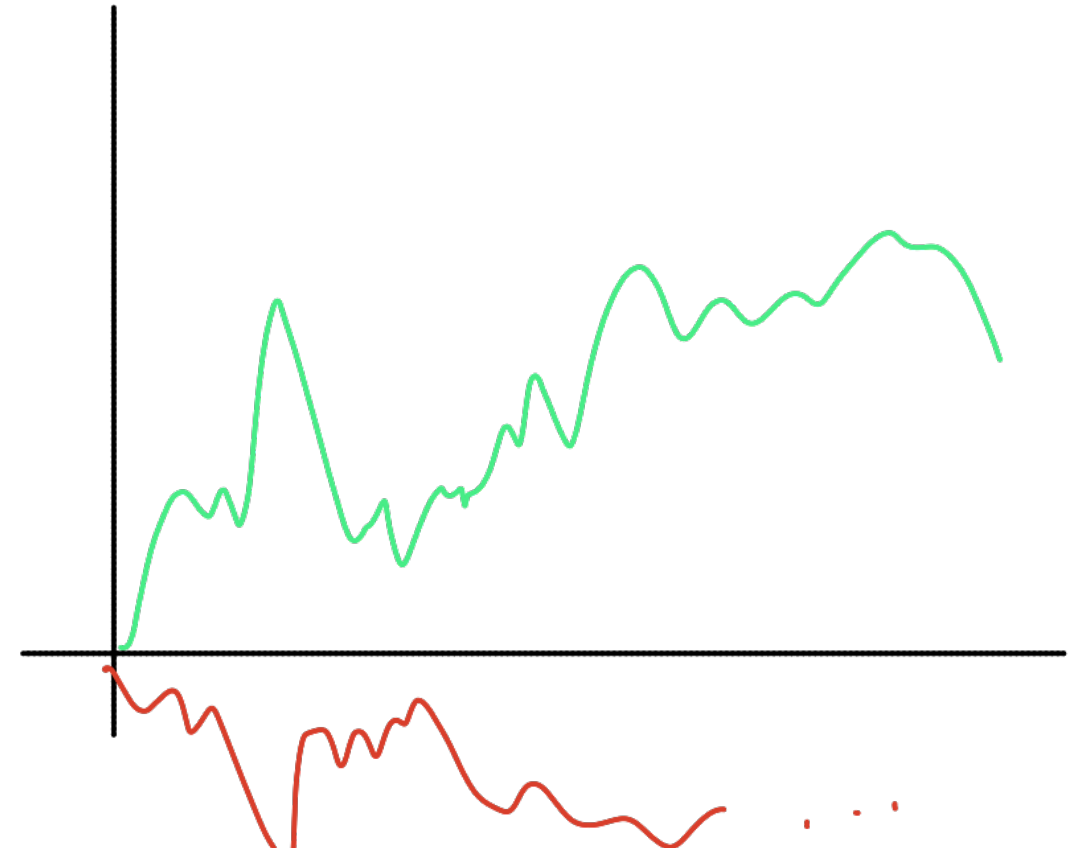
\includegraphics[width=0.4\linewidth]{img/screenshot011}
		\caption{I am sorry, I cut the screenshot.}
		\label{fig:screenshot011}
	\end{figure}
	\item \emph{Renewal} (or \emph{time deletion}): let ${(B_{t})}_{t\geq0}$ be a $\mathrm{BM}^{d}$. Fix a time $a>0$ and define the process ${(W_{t})}_{t\geq0}$ as
	\begin{equation*}
		W_{t}:=B_{t+a}-B_{a}.
	\end{equation*}
	Then ${(W_{t})}_{t\geq0}$ is again a $\mathrm{BM}^{d}$.
	\begin{figure}[H]
		\centering
		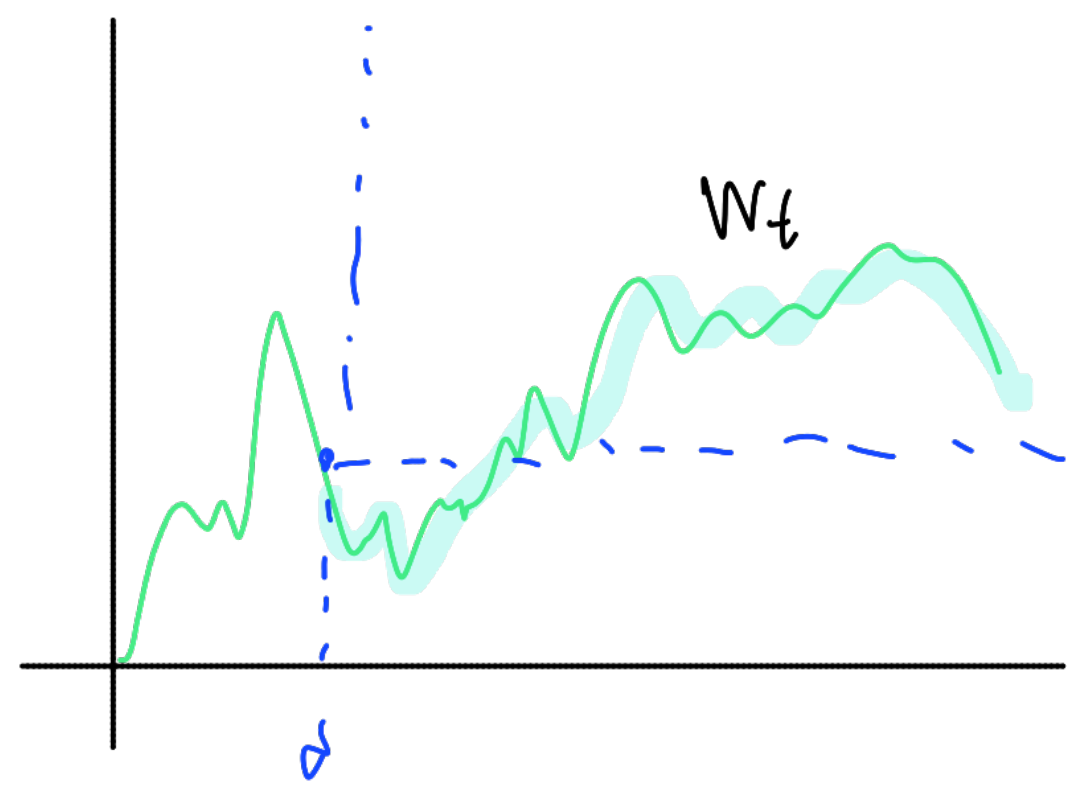
\includegraphics[width=0.4\linewidth]{img/screenshot012}
		\caption{I am sorry, I didn't make the lines straight.}
		\label{fig:screenshot012}
	\end{figure}
	\begin{fancyproof}
		\begin{enumerate}
			\item[1.] We know $W_{0}=0$.\hspace*{\fill}\faCheckCircle
			\item [2.-3.] If $t_{0}=0<t_{1}<\ldots<t_{n}$ then
			\begin{align*}
				W_{t_{h}}-W_{t_{j-1}}&=B_{t_{j}+a}-\cancel{B_{a}}-B_{t_{j-1}+a}+\cancel{B_{a}}\\
				&=B_{t_{j}-a}-B_{t_{j-1}+a}\distnorm{0,t_{j}-t_{j-1}}
			\end{align*}
			so the independence of the increments and their stationarity follows from those of $B_{t}$.\hspace*{\fill}\faCheckCircle
			\item[4.] The continuity is obvious since the sample paths coincide after $a$.\hspace*{\fill}\faCheckCircle
		\end{enumerate}
	\end{fancyproof}
	\begin{lemma}
		$W_{t}=B_{t+a}-B_{a}$ and $B_{t},t\in(0,a)$ are independent.
	\end{lemma}
	\item \emph{Time inversion}: take $W_{t}:=B_{\tau-t}-B_{t}$ for $t\in[0,\tau]$.
	\begin{figure}[H]
		\centering
		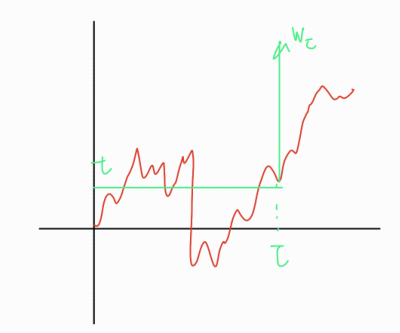
\includegraphics[width=0.5\linewidth]{img/screenshot013}
		\caption{This drawing is not very clear to me either.}
		\label{fig:screenshot013}
	\end{figure}
	If $B_{t}$ is a BM we get another BM inverting time.
	\item \emph{Scaling property}: if $c$ is a constant then 
	\begin{equation*}
		B_{ct}\sim c^{\sfrac{1}{2}}B_{t}
	\end{equation*}
	so if I change the scale in which I measure the time I get another BM.
	\begin{equation*}
		W_{t}={(c^{\sfrac{1}{2}}B_{ct})}_{t\geq 0}
	\end{equation*}
	is a $\mathrm{BM}^{d}$ and
	\begin{equation*}
		\mathsf{N}(0,ct)=\sqrt{c}\mathsf{N}(0,t).
	\end{equation*}
	\item \emph{Projective reflection} at $t=\infty$: let $B_{t}$ be a $\mathrm{BM}^{d}$. Let 
	\begin{equation*}
		W_{t}=\begin{cases}
			tB_{\frac{1}{t}}&t>0\\
			0&t=0.
		\end{cases}
	\end{equation*}
	$W_{t}$ is again a $\mathrm{BM}^{d}$.
	\begin{fancyproof}
		We must use the Gaussian definition: consider the vector
		\begin{equation*}
			W=\left(W_{t_{1}},W_{t_{2}},\ldots,W_{t_{n}}\right) \qquad0\leq t_{1}<\ldots<t_{n}
		\end{equation*}
		which is a Gaussian vector. Now, we know that 
		\begin{enumerate}
			\item $\evs[W]=0$;
			\item \begin{align*}
				\cov\left[W_{t_{j}},W_{t_{k}}\right]&=\cov\left[t_{j}B_{\frac{1}{t_{j}}},t_{k}B_{\frac{1}{t_{k}}}\right]\\
				&=t_{j}t_{k}\cov\left[B_{\frac{1}{t_{j}}},B_{\frac{1}{t_{k}}}\right]\\
				&=t_{j}t_{k}\left(\frac{1}{t_{j}}\wedge\frac{1}{t_{k}}\right)=t_{j}\wedge t_{k}.
			\end{align*}
				\end{enumerate}
				So this process has the mean and variance of a BM!
			To check the continuity of sample paths we know that for $t\geq0$ then $t\mapsto W_{t}$ is a continuous function... but we must also prove the continuity at 0! (Durret p. 363).
			We can rewrite $B_{n}$ as
			\begin{equation*}
				B_{n}=B_{1}+(B_{2}-B_{1})+\ldots+(B_{n}-B_{n-1}).
			\end{equation*}
			This is a sum of i.i.d. \rv s. We can use the Law of Large Numbers to consider the limit of the sum
			\begin{equation*}
				\lim_{n\to\infty}\frac{B_{n}}{n}=\evs[B_{t}]=0
			\end{equation*}
			This means that the fluctuations of $B_{n}$ become more and more irrelevant with respect to $n$ and this means that there is a tendency over time to smooth to 0. So the limit through the integer converges to 0... But we are interested in the real numbers, not just the integers! Remember Kolmogorov's maximal inequality:
			\begin{revise}
				\begin{equation*}
					\pr\left(\max_{k\leq n}|S_{k}|\geq x\right)\leq\frac{\var S_{n}}{x^{2}}.
				\end{equation*}
			\end{revise}
			As $k$ we take the interval of size 1 over $n$:
			\begin{equation*}
				\pr\left(\sup_{k}\left|B_{n+\frac{k}{n^{m}}}-B_{n}\right|\geq n^{\sfrac{2}{3}}\right)\leq\overbracket{\frac{\evs\left[\left(B_{n+1}-B_{n}\right)^{2}\right]}{n^{\sfrac{2}{3}}}}^{\claptext{if mean is 0 then variance is just second moment}}.
			\end{equation*}
			\begin{figure}[H]
				\centering
				
\includegraphics[width=0.5\linewidth]{img/screenshot014}
				\caption{WHERE THE FUCK DID $m$ COME FROM??}
				\label{fig:screenshot014}
			\end{figure}
			This is like breaking the interval between $n$ and $n+1$ into finer and finer pieces.
			Now let $m\to\infty$:
			\begin{equation*}
				\pr\left(\sup_{u\in[n,n+1]}|B_{u}-B_{n}|>n^{\sfrac{2}{3}}\right)\leq n^{-\sfrac{4}{3}}.
			\end{equation*}
			This is like asking the probability of the event ``at least once between time $n$ and $n+1$, the Brownian motion jumps too much (more than $n^{\sfrac{2}{3}}$)''. Using Kolmogorov we can say that this probability will be at most $n^{-\sfrac{4}{3}}$. But we know that $\sum_{n}n^{-\sfrac{4}{3}}<\infty$ so we can apply Borel Cantelli to get that 
			\begin{equation*}
				\frac{B_{u}}{u}\to 0.
			\end{equation*}
			Now take $u=\frac{1}{t}$ and get the result.
	\end{fancyproof}
\end{enumerate}
\section{Martingales related with \bwm}
\subsection{Three \textcolor{Gold3}{golden} martingales}
\begin{definition}
	A martingale $(X_{t},\F_{t})$ is a real or complex stochastic process
	\begin{equation*}
	\begin{array}{lc}
		X_{t}:\Omega\to\R^{d}&\mathrm{or}\\
		X_{t}:\Omega\to\mathbb{C}
	\end{array}
	\end{equation*}
	satisfying
	\begin{enumerate}
		\item $\evs|X_{t}|\leq\infty$ for $\every t\in\T$;
		\item $X_{t}$ is $\F_{t}$-measurable for $\every t\in\T$;
		\item $\evs\left[X_{t}|\F_{s}\right]=X_{s}$ for $\every s,t\in\T$ and $s<t$.
	\end{enumerate}
\end{definition}
This is nothing new from what we already knew. We just added the complex definition because we may want to work with the characteristic functions. 
\newtcolorbox{gold}[1]{enhanced jigsaw, interior style={shade, ball color=Gold1!40},breakable,coltitle=white,colbacktitle=Gold4, title = #1, colframe=black, fonttitle=\bfseries,sharp corners}
\begin{gold}{Three golden martingales}
	\begin{enumerate}
		\item ${(B_{t})}_{t\geq0}$;
		\item ${(B_{t}^{2}-t)}_{t\geq 0}$ (or $B_{t}^{2}-\dt$ if $B_{t}$ is a $\mathrm{BM}^{d}$);
		\item ${\left(e^{\sigma B_{t}-\frac{\sigma^{2}}{2}t}\right)}_{t\geq 0}$.
	\end{enumerate}
\end{gold}
\begin{exercise}
	Check that the \bwm{} with drift is a sub-martingale if $\mu$ is positive.
\end{exercise}
\begin{fancyproof}
\begin{enumerate}
		\item \begin{enumerate}
		\item We know that $B_{t}\sim N(0,t)$ hence $|B_{t}|$ has p.d.f.
		\begin{equation*}
			f_{|B_{t}|}(y)=\frac{\sqrt{2}}{\sqrt{\pi t}}e^{-\frac{y^{2}}{2t}}.
		\end{equation*}
		Hence, it has expectation
		\begin{align*}
			\evs|B_{t}|&=\int_{0}^{\infty}f_{|B_{t}|}(y)\dy\\
			&=\sqrt{\frac{2}{\pi t}}t\int_{0}^{\infty}y\cdot\frac{1}{t}\cdot e^{-\frac{y^{2}}{2t}}\dy\\
			\text{change of variable: }&u=\frac{y^{2}}{2t}\implies \du=\frac{y}{t}\dy\implies\dy=\du\frac{t}{y}\\
			&=\sqrt{\frac{2t}{\pi}}\ubracketthin{\int_{0}^{\infty}e^{-u}\du}_{=1}\\
			&=\sqrt{\frac{2t}{\pi}}<\infty
		\end{align*}
		or, if you hate yourself, note that the integrand is... kinda like the derivative of the exponential term. Indeed,
		\begin{align*}
\dif\left(e^{-\frac{y^{2}}{2t}}\right)
			&=e^{-\frac{y^{2}}{2t}}\dif\left(-\frac{y^{2}}{2t}\right)\\
			&=-e^{-\frac{y^{2}}{2t}}\cdot\frac{y}{t}\dy
		\end{align*}
		so we can write
		\begin{equation*}
				\sqrt{\frac{2t}{\pi}}\int_{0}^{\infty}y\cdot\frac{1}{t}\cdot e^{-\frac{y^{2}}{2t}}\dy=\sqrt{\frac{2t}{\pi}}\int_{0}^{\infty}-\dif\left(e^{-\frac{y^{2}}{2t}}\right)
		\end{equation*}
	so using the fundamental theorem of calculus $\int_{0}^{\infty}\dif F(y)=F(\infty)-F(0)$ we get
	\begin{equation*}
		\sqrt{\frac{2t}{\pi}}\cdot-\left[e^{\frac{-y^{2}}{2t}}\right]^{y=\infty}_{y=0}\implies\sqrt{\frac{2t}{\pi}}\cdot-(0-1)=\sqrt{\frac{2t}{\pi}}<\infty
	\end{equation*}
		So it is integrable. 
		\begin{insult}
			On a totally unrelated tangent, I spent 2 hours over this stupid fucking equation because during the lessons \textit{someone} decided that there was not a minus sign. Also what the fuck is this notation of $\dif({\text{my shit}})$? Never seen this before and almost had an aneurysm. After all of this, turns out it is just a lazy way to not evaluate an integral.
		\end{insult}
		\item It is $\F_{t}^{B}$ measurable.
		\item To check if it is a martingale: 
		\begin{align*}
			\evs[B_{t}|\F_{s}]&=\evs[B_{t}-B_{s}+B_{s}|\F_{s}]\\
			&=\ubracketthin{\evs[B_{t}-B_{s}|\F_{s}]}_{\claptext{$= 0$ because they are increments of BM}}+B_{s}=B_{s}
		\end{align*}
		so it is a martingale.
	\end{enumerate}
	\item Consider $M_{t}=|B_{t}|^{2}$ where $B_{t}$ is $\mathrm{BM}^{d}$. We need to show that $M_{t}$ is a sub-martingale with respect to $\F_{t}$.
	\begin{enumerate}
		\item[(a)-(b)] These are easy. I think.
		\item[(c)]\begin{align*}
			\evs[M_{t}|\F_{t}]&=\sum_{j=1}^{d}\evs\left[{\left(B_{t}^{j}\right)}^{2}\big|\F_{s}\right]\\
			&\geq\sum_{j=1}^{d}\left(\evs\left[B^{j}_{t}|F_{s}\right]\right)^{2}\\
			&=\sum_{j=1}^{d}\left(B^{j}_{s}\right)^{2}.
		\end{align*}
		Now let's move to the quantity of interest
		\begin{equation*}
			M_{t}=|B_{t}|^{2}-\dt=\sum_{j=1}^{d}\left[{(B^{j}_{t})}^{2}-t\right]
		\end{equation*}
		hence it is enough to prove the result for $d=1$. Consider $s<t$ and $\evs\left[B^{2}_{t}-t|\F_{s}\right]$.
		\begin{align*}
			\evs\left[B^{2}_{t}-t|\F_{s}\right]&=\evs\left[\Bigl(\bigl(B_{t}-B_{s}\bigr)+B_{s}\Bigr)^{2}-t|\F_{s}\right]\\
			&=\evs\left[(B_{t}-B_{s})^{2}+B_{s}^{2}+2B_{s}(B_{t}-B_{s})-t|\F_{s}\right]\\
			&=\ubracketthin{\evs\left[(B_{t}-B_{s})^{2}|\F_{s}\right]}_{t-s}-t+B_{s}^{2}-2B_{s}\ubracketthin{\evs\left[B_{t}-B_{s}|\F_{s}\right]}_{0}\\
			&=B_{s}^{2}-t
		\end{align*}
		so the process is a martingale!
	\end{enumerate}
	\item Consider $M_{t}:=e^{i\langle\lambda,B_{t}\rangle+\frac{t}{2}|\lambda^{2}|}$ for $\lambda\in\R^{d}$. This is the same case as written above, but this time we are in the complex realm. Consider the expectation
	\begin{align*}
		\evs[M_{t}^{\lambda}|\F_{s}]&=e^{\frac{t}{2}|\lambda^{2}|}\evs\left[e^{i\inprod{\lambda,B_{t}-B_{s}+B_{s}}}|\F_{s}\right]\\
		&=e^{\frac{t}{2}|\lambda^{2}|}\ubracketthin{\evs\left[e^{i\inprod{\lambda, B_{t}-B_{s}}}|\F_{s}\right]}_{B_{t}-B_{s}\independent\F_{s}}e^{i\inprod{\lambda, B_{s}}}\\
		&=e^{\frac{t}{2}|\lambda^{2}|}e^{i\inprod{\lambda, B_{s}}}\evs\Bigl[e^{i\inprod{\lambda,\overbracket{B_{t}-B_{s}}^{B_{t-2}}}}\Bigr]\\
		&=e^{\frac{t}{2}|\lambda^{2}|}e^{i\inprod{\lambda,B_{s}}}\ubracketthin{e^{-\frac{t-s}{2}\lambda^{2}}}_{\claptext{characteristic function of $\mathsf{N}(0,t-s)$}}.
	\end{align*}
\end{enumerate}
\end{fancyproof}
Well. But what is the point of any martingale in general? For example, consider
\begin{equation*}
	\pr\left(\sup_{0<t<\theta}B_{t}\geq b\right)\leq\exp\left\{-\frac{b^{2}}{2\theta}\right\}.
\end{equation*}
This means that the probability that the \bwm{} exceeds a certain value $b$ at any point in time in the interval $(0,\theta)$ decreases exponentially with $\frac{b^{2}}{\theta}$, which means that the probability of the \bwm{} reaching or exceeding a large value $b$ in the interval decreases rapidly as $b$ increases or $\theta$ (the time window) becomes large. We will be able to improve this estimation of the probability paths, but this is a simple result obtained from martingale properties.\\
We can use Doob's maximal inequality. Consider
\begin{align*}
	\pr\left(\sup_{0<t<\theta}B_{t}\geq b\right)&\stackrel{\lambda>0}{=}\pr\left(e^{\lambda B_{t}}\geq e^{\lambda t}\right)\\
	&\leq\frac{\evs\left[\lambda B_{\theta}\right]}{e^{\lambda b}}\\
	&=\exp\left\{\unmezz\lambda^{2}\theta\right\}e^{-\lambda b}.
\end{align*}
Since $\lambda>0$ is arbitrary, we choose $\lambda$ to minimize the right hand side. The result is 
\begin{equation*}
	\lambda=\frac{b}{\theta}.
\end{equation*}
Remind that if $M$ is a martingale in $\lp$, $p>1$ and $\frac{1}{p}+\frac{1}{q}=1$ then
\begin{equation*}
	\evs\max_{k\in(1,n)}|M_{k}|^{p}\leq q^{p}\evs\left[|M_{n}|^{p}\right].
\end{equation*}
This inequality holds true also for continuous time. Let's apply it to BM:
\begin{equation*}
	\evs\left[\sup_{0<s<\theta}|B_{s}|^{p}\right]\leq\left(\frac{p}{p-1}\evs\left[|B_{t}|^{p}\right]\right).
\end{equation*}
Of course $\frac{1}{q}=1-\frac{1}{p}\implies q=\frac{p}{p-1}$.
\begin{definition}
	Take a filtration $\F=(\F_{t})$. We say that it is \emph{augmented} if $(\Omega,\HS,\pr)$ is complete (i.e. each negligible set is measurable) and all negligible events in $\HS$ are also in $\F_{0}$ (and hence in $\F_{t}$).
\end{definition}
\begin{definition}
	Let $\F$ be a filtration. Define
	\begin{equation*}
		\F_{t^{+}}=\bigcap_{\varepsilon>0}\F_{t+\varepsilon}\qquad t\in\R^{+}.
	\end{equation*}
\end{definition}
In this case $\F_{t^{+}}$ is again a filtration and it is finer than $\F_{t}$. Imagine we want to compute
\begin{equation*}
	v_{t}=\lim_{\varepsilon\to0}\frac{x_{t+e}-x_{t}}{\varepsilon}
\end{equation*}
which is like calculating the velocity of $X$ (given the position), where we need an infinitesimal quantity of information beyond $t$. This is what the filtration $\F_{t^{+}}$ tells us. $v_{t}$ is defined on $\F_{t^{+}}$ but not on $\F_{t}$.
\begin{definition}
	If $\F_{t}=\F_{t^{+}},\; t\in\R^{+}$, the filtration is said to be \emph{right continuous}.
\end{definition}
For example, the Levy process does not have a right continuous filtration.
\begin{figure}[H]
	\centering
	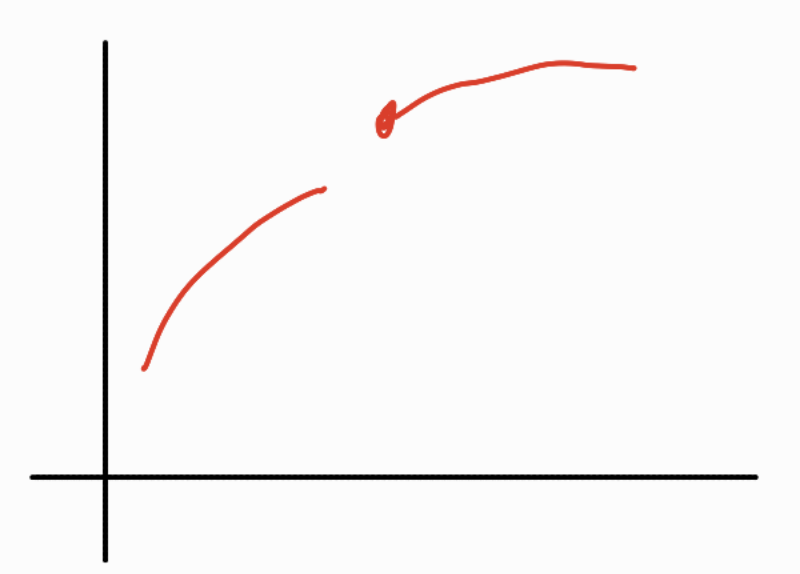
\includegraphics[width=0.5\linewidth]{img/screenshot015}
	\caption{It's broken!}
	\label{fig:screenshot015}
\end{figure}
On the other hand, BM has right-continuous natural filtration.\par
Consider two continuous positive \rv s $T, V$. Define
\begin{equation*}
	X_{t}(\omega)=\begin{cases}
		V(\omega)t&t<T(\omega)\\
		V(\omega)T(\omega)&t\geq T(\omega).
	\end{cases}
\end{equation*}
We are describing, for example, the motion of a particle that moves from the origin with speed $V$ until $T$ and then stops after $T$. Consider the filtration generated by $X$. Is $T$ a stopping time of $\F$? When $X_{s}(\omega)=V(\omega)s$ we still don't know if $T(\omega)=s$ or $T(\omega)>s$... but
\begin{equation*}
	\left\{T\leq t\right\}\in\F_{t+\varepsilon\every \varepsilon>0}\implies\left\{T\leq t\right\}\in\F_{t^{+}}.
\end{equation*}
We know that with continuous distributions, $T=t$ has probability 0... but this doesn't mean that the object doesn't exists, just that it is negligible. 
\subsection{Boundaries of BM}
Consider
\begin{equation*}
	\begin{array}{ll}
		\tau^{0}_{A}:=\left\{t\geq0:X_{t}\in A\right\}&\text{\emph{first entry time in $A$}.}\\
		\tau_{A}:=\inf\left\{t>0:X_{t}\in A\right\}&\text{\emph{first hitting time in $A$}.}\\
		\tau_{A^{c}}:=\inf\left\{t\geq0:X_{t}\notin A\right\}&\text{\emph{first exit time from $A$}.}
	\end{array}
\end{equation*}
If the inferior is the null set we say $\inf\left\{\emptyset\right\}=\infty$ and
\begin{equation*}
	\tau^{0}_{A}\leq\tau_{A}.
\end{equation*}
\begin{lemma}
	Consider a $d$-dimensional stochastic process $\{X_{t}\}$ with continuous sample paths and $A\subset\R^{d}$ closed. Then $\tau_{A}^{0}$ is an $\F_{t}^{X}$ stopping time and $\tau_{A}$ is an $\F_{t^{+}}^{X}$ stopping time.
\end{lemma}
The difference is  that $\tau_{A}^{0}$ includes the 0, while $\tau_{A}$ doesn't. We must have a peek of what comes next. \par
Let's take into consideration the one dimensional case. Consider $\tau_{b}:=\tau_{\{b\}}^{0}$, the first entry time into the closed set $\{b\}$. Our problem consists in looking when the BM crosses the boundary $b$. Will it even do it? We are asking 
\begin{equation*}
	\pr(\tau_{b}<\infty)=?
\end{equation*}
In other words, is it a sure event?
\begin{figure}[H]
	\centering
	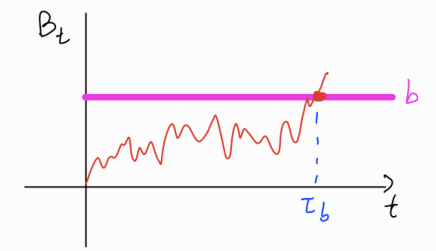
\includegraphics[width=0.5\linewidth]{img/screenshot016}
	\caption{Wasn't $b$ a set? I don't even care anymore.}
	\label{fig:screenshot016}
\end{figure}
In general, $X_{t}$ can be a continuous stochastic process and $b$ can depend on time (being a function $b(t)$).
\begin{figure}[H]
	\centering
	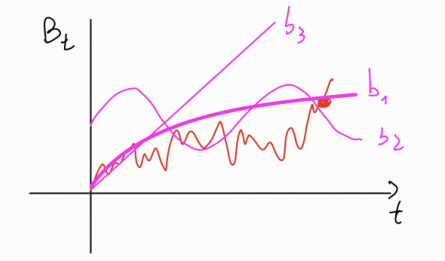
\includegraphics[width=0.5\linewidth]{img/screenshot017}
	\caption{The point of entry shouldn't be the same for all three functions but you hopefully get the point.}
	\label{fig:screenshot017}
\end{figure}
Sometimes we may be able to prove analitically how $\tau_{b(t)}$ is distributed, sometimes not. What we care about now is to understand whether it even passes the threshold. For example. GPS satellites works using atomic clocks to triangulate the position and a small error in time can completely fuck your position up. Atomic clocks must always be aligned and one of the models used to compute the error of the clocks is the integral of \bwm, so yeah. Is pretty important to know how this bitch behaves.
\begin{remark}
	Of course, 
	\begin{equation*}
		\sup_{t\geq0}B_{t}\geq\sup_{n\geq 1}B_{n}
	\end{equation*}
	since if I start to consider the process earlier I will get at least the maximum I would obtain if I started later. But
	\begin{equation*}
		\sup_{n\geq 1}B_{n}=\sup_{n\geq 1}(\xi_{1}+\xi_{2}+\ldots+\xi_{n})
	\end{equation*}
	with $\xi_{i}=(B_{i}-B_{i-1})$ i.i.d. by definition of \bwm. Now define
	\begin{equation*}
		S:=\sup_{n\geq 1}\sum_{i=1}^{n}\xi_{i}=\xi_{1}+\sup_{n\geq 1}\sum_{i=1}^{n}\xi_{i}=\xi_{1}+S'.
	\end{equation*}
	Note that
	\begin{itemize}
		\item $\xi_{i}$'s are i.i.d. so $S\sim S'$;
		\item $\xi_{1}$ is independent from $S'$;
		\item $\xi_{1}$ is not trivial, so it is not 0.
	\end{itemize}
	But this means that $S=\infty$ \as{} because this would be the only case in which the sum stays the same after I add a non-trivial quantity!\\
	We can apply the same idea to the infimum and say that
	\begin{equation*}
		\pr(\sup_{t\geq 0} B_{t}=\infty,\inf_{t\geq 0} B_{t}=-\infty)=1.
	\end{equation*}
\end{remark}
	This remark means that 
\begin{equation*}
	\pr(\tau_{b}<\infty)=1
\end{equation*}
because if I can go from $-\infty$ to $\infty$ then I cross every value at least twice!
\begin{figure}[h]
	\centering
	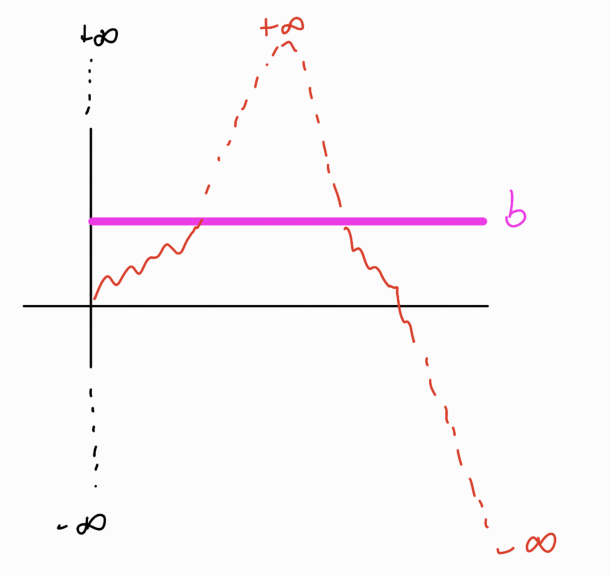
\includegraphics[width=0.6\linewidth]{img/screenshot018}
	\caption{Now the lines are more straight, c'mon.}
	\label{fig:screenshot018}
\end{figure}
This means that I can ``split'' the process at every level $b$. Not only that, but it will cross the threshold of $b$ infinitely often since it has to go to and fro infinity infinite times! Like Markov chains, \bwm{} is \emph{point recurrent}: each time the process leaves a state $b$ it will return there sooner or later.\\
We proved that \bwm{} has the martingale property. We will now use the Doob's optional stopping theorem.
\begin{theorem}
	\emph{Doob's optional stopping theorem}. Let $M$ be a stochastic process adapted to $\F$. The following are equivalent:
	\begin{enumerate}
		\item $M$ is a $\F$-submartingale.
		\item For every bounded stopping times $S,T$ with $S\leq T$ the \rv s $M_{S}$ and $M_{T}$ are integrable and 
		\begin{equation*}
			\evs_{S}\left[M_{T}-M_{S}\right]\geq0.
		\end{equation*}
	\end{enumerate}
\end{theorem}
	This means that the conditional expectation satisfies the submartingale property even after stopping.
	\begin{theorem}
		\emph{Wald's identity}. Let $(B_{t},\F_{t})$ be a $\mathrm{BM}^{1}$ and assum that $\tau$ is a $\F_{t}$ stopping time. If $\evs\tau<\infty$ then $B_{\tau}\in L^{2}$ and
		\begin{equation*}
			\begin{array}{c}
				\evs B_{\tau}=0\\
				\evs B_{\tau}^{2}=\evs\tau.
			\end{array}
		\end{equation*}
	\end{theorem}
	Here we are relating a second moment with a first moment expectation. This tells us that the expectation of the \bwm{} is 0 also on stopping times (we already saw this with deterministic times) and its variance is equal to the mean value of $\tau$.
	\begin{fancyproof}
		We need Doob's stopping theorem. Introduce ${(\tau\wedge t)}_{t\geq0}$: this gives us a bounded stopping time for Doob's Stopping theorem. 
		\begin{enumerate}
			\item We know that $(B_{\tau\wedge t},\F_{\tau\wedge t})$ is a martingale and
			\begin{equation*}
				\evs B_{\tau\wedge t}=\evs B_{0}=0.
			\end{equation*}
			\item We must prove that $B_{\tau}\in L^{2}$. Use the inequality of the maximum:
			\begin{equation*}
				\evs\left[\sup_{s\leq t}|B_{s}|^{p}\right]\leq\left(\frac{p}{p-1}\right)^{p}\evs|B_{t}|^{p}.
			\end{equation*}
			Choose $p=2$. We have
			\begin{equation*}
				\evs\left[B^{2}_{\tau\wedge t}\right]\leq\evs\left[\sup_{s\leq t}B^{2}_{s}\right]\leq 4\evs\left[B^{2}_{t}\right]=4t
			\end{equation*}
			hence
			\begin{equation*}
				B_{\tau\wedge t}\in L^{2}.
			\end{equation*}
			\item Use Doob's optional stopping theorem applies to the $\F_{\tau\wedge t}$ martingale: define
			\begin{equation*}
				M^{2}_{t}:=B^{2}_{\tau\wedge t}-\tau\wedge t
			\end{equation*}
			so that 
			\begin{equation*}
				\evs M^{2}_{t}=\evs M^{2}_{0}=0\implies \evs\left[B^{2}_{\tau\wedge t}\right]=\evs\left[\tau\wedge t\right].
			\end{equation*}
			We now need to remove $t$. We have to find a $L^{2}$ Cauchy sequence to prove that there is a limit that we can take.
			\begin{remark}
				For all $s\leq t$ we have that
				\begin{equation*}
					\evs\left[B_{\tau\wedge t}B_{\tau\wedge s}\right]=\evs\left[B^{2}_{\tau\wedge s}\right].
				\end{equation*}
			\end{remark}
			So
			\begin{align*}
				\evs\left[\left(B_{\tau\wedge t}-B_{\tau\wedge s}\right)^{2}\right]&=\evs\left[B^{2}_{\tau\wedge t}+B^{2}_{\tau\wedge s}-2B^{2}_{\tau\wedge s}\right]\\
				&=\evs\left[B^{2}_{\tau\wedge t}-B^{2}_{\tau\wedge s}\right]\\
				&=\evs\left[\tau\wedge t-\tau\wedge s\right]\xrightarrow[]{s,t\to\infty}0.
			\end{align*}
			So $\left(B_{\tau\wedge t}\right)$ is an $L^{2}$ Cauchy sequence. Furthermore, we know that $\tau<\infty$ a.s. by hypothesis and we know that $B_{t}$ has continuous samples, so we can get almost sure convergence:
			\begin{equation*}
				L^{2}-\lim_{t\to\infty}B_{\tau\wedge t}=B_{\tau}.
			\end{equation*}
			Using the fact that $B_{\tau}\in L^{2}$ and using the monotone convergence theorem we get that 
			\begin{equation*}
				\evs\left[B^{2}_{\tau}\right]=\lim_{t\to\infty}\evs\left[B^{2}_{\tau\wedge t}\right]=\lim_{t\to\infty}\evs[\tau\wedge t]=\evs[\tau].
			\end{equation*}
			Finally, $L^{2}$ convergence implies $\lone$ convergence:
			\begin{equation*}
				\evs B_{\tau}=\lim_{t\to\infty}B_{\tau\wedge t}=0.
			\end{equation*}
		\end{enumerate}
	\end{fancyproof}
	\begin{corollary}
		Let ${(B_{t})}_{t\geq0}$ be a one-dimensional \bwm{} and let 
		\begin{equation*}
			\tau:=\inf_{t\geq 0}\left\{t\geq0:B_{t}\notin(-a,b)\right\}
		\end{equation*}
		be the first entry time into the set $(-a,b)^{C}$ with $a,b\geq 0$.
		\begin{figure}[H]
			\centering
			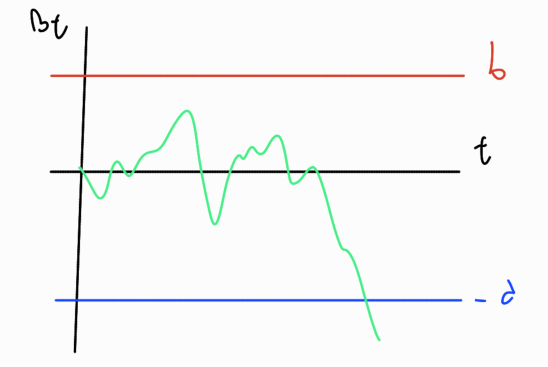
\includegraphics[width=0.5\linewidth]{img/screenshot019}
			\caption{I completely tuned out from this part of the lecture on.}
			\label{fig:screenshot019}
		\end{figure}
		Then
		\begin{equation*}
			\begin{array}{rl}
				\pr(B_{\tau}=-a)&=\frac{b}{a+b}\\
				\pr(B_{\tau}=b)&=\frac{a}{a+b}\\
				\evs\tau&=ab.
			\end{array}
		\end{equation*}
	\end{corollary}
\begin{fancyproof}
	We know that $\tau\wedge t$ is a bounded stopping time and that $B_{\tau\wedge t}\in[a,b]$: hence
	\begin{equation*}
		|B_{\tau\wedge t}|\leq a\vee b.
	\end{equation*}
	But by the previous theorem we know that 
	\begin{equation*}
		\evs[\tau\wedge t]=\evs\left[B^{2}_{\tau\wedge t}\right]\leq a^{2}\vee b^{2}.
	\end{equation*}
	Now use the monotone convergence theorem to get that
	\begin{equation*}
		\evs\tau\leq a^{2}\vee b^{2}\leq\infty.
	\end{equation*}
	From Wald's identities we have that 
	\begin{equation*}
		\begin{array}{c}
			\evs B_{t}=0\\
			-a\pr(B_{\tau}=-1)+b\pr(B_{\tau}=b)=0.
		\end{array}
	\end{equation*}
	Furthermore, we know
	\begin{equation*}
		\pr(B_{\tau}=-a)+\pr(B_{\tau}=b)=1.
	\end{equation*}
	So we have a nice little system that we can solve to get
			\begin{equation*}
		\begin{array}{rl}
			\pr(B_{\tau}=-a)&=\frac{b}{a+b}\\
			\pr(B_{\tau}=b)&=\frac{a}{a+b}.
		\end{array}
	\end{equation*}
	Now use the second Wald's identity to get that 
	\begin{align*}
		\evs_{\tau}&=\evs B^{2}_{\tau}\\
		&=a^{2}\pr(B_{\tau}-a)+b^{2}\pr(B_{\tau}=b)\\
		&=a^{2}\frac{b}{a+b}+b^{2}\frac{a}{a+b}\\
		&=ab.
	\end{align*}
\end{fancyproof}
\begin{remark}
	If $a\to\infty$ (which means we are in the one boundary case, or the \textit{absorbing barrier} case):
	\begin{enumerate}
		\item $\pr(B_{\tau}=b)=\lim_{a\to\infty}\frac{a}{a+b}=1$;
		\item if we want
		\begin{equation*}
			\tau_{1}=\inf_{t\geq 0}\{t\geq0:B_{t}=1\}
		\end{equation*}
		then we have 
		\begin{equation*}
			\evs\tau_{1}=\lim_{a\to\infty}ab=\infty.
		\end{equation*}
		This means heavy tails for the distribution of this stopping time.
	\end{enumerate}
\end{remark}
Remember that the one-dimensional \bwm{} is recurrent, meaning that it visits 1 infintely often... but the time to attain 1 diverges. \begin{fancyproof}
	We know that 
\begin{equation*}
	\tau<\infty\qquad\as{}
\end{equation*}
and
\begin{equation*}
	\B_{\tau_{1}}=1\text{ and }\evs B_{\tau_{1}}=\evs B^{2}_{\tau_{1}}=1.
\end{equation*}
This means that
\begin{equation*}
	\evs{\tau}=\infty.
\end{equation*}
\end{fancyproof}
\section*{Exercises}
\label{sec:exer2}
\addcontentsline{toc}{section}{\nameref{sec:exer2}}
\begin{exercise}
	Let ${(B_{t})}_{t\geq 0}$ be a Brownian motion in dimension 1 on $(\Omega,\F,\pr)$ and let ${(\R_{t})}_{t\geq 0}$ be its natural filtration. Define
	\begin{equation*}
		X_{t}:=\int_{0}^{t}B_{s}\ds
	\end{equation*}
	and
	\begin{equation*}
		M_{t}:=X_{t}-\frac{1}{3}B_{t}^{3}.
	\end{equation*}
	Prove that:
	\begin{enumerate}
		\item $\ev{B^{3}_{t}|\F_{s}}=B^{3}_{s}+3B_{s}(t-s)$;
		\item $\ev{\int_{s}^{t}B_{u}\du|\F_{s}}=(t-s)B_{s}$. Hint: use the following result
		\begin{equation*}
			\ev{\int_{s}^{t} Y_{u}\du|\G}=\int_{s}^{t}\ev{Y_{u}|\G}\du
		\end{equation*}
		that holds for each $0\leq s\leq t$ and each \sa{} $\G\subset\F$ and each process $Y={(Y_{u})}_{u\in(0,\infty)}$ continuous and with $Y_{u}^{2}\in L^{2}$;
		\item $M$ is a martingale.
	\end{enumerate}
\end{exercise}
\begin{enumerate}
	\item We know that
	\begin{align*}
		\ev{B^{3}_{t}|\F_{s}}&=\ev{\left((B_{t}-B_{s})+B_{s}\right)^{3}|\F_{s}}\\
		&=\evBig{\ubracketthin{B^{3}_{s}}_{\claptext{$\F_{s}$-meas}}+3\ubracketthin{B_{s}}_{\claptext{$\F_{s}$-meas}}(B_{t}-B_{s})^{2}+3\ubracketthin{B_{s}^{2}}_{\claptext{$\F_{s}$-meas}}(B_{t}-B_{s})+(B_{t}-B_{s})^{3}|\F_{s}}\\
		&=B_{s}^{3}+3B_{s}\evBig{\ubracketthin{(B_{t}-B_{s})^{2}}_{\claptext{$\independent$ from $\F_{s}$}}|\F_{s}}+3B_{s}^{2}\evBig{\ubracketthin{B_{t}-B_{s}}_{\claptext{$\independent$ from $\F_{s}$}}|\F_{s}}+\evBig{\ubracketthin{(B_{t}-B_{s})^{3}}_{\claptext{$\independent$ from $\F_{s}$}}|\F_{s}}\\
		&=B_{s}^{3}+3B_{s}\ubracketthin{\ev{(B_{t}-B_{s})^{2}}}_{t-s}+3B_{s}^{2}\ubracketthin{\ev{B_{t}-B_{s}}}_{0}+3\ubracketthin{\ev{B_{t}-B_{s}}^{2}}_{0}\\
		&=B^{3}_{s}+3B_{s}(t-s).
	\end{align*}
	\item Using the suggested hint we get:
	\begin{align*}
		\ev{\int_{s}^{t}B_{u}\du|\F_{s}}&=\int_{s}^{t}\evs[{\ubracketthin{B_{u}|\F_{s}}_{\claptext{$\independent$ from $\F_{s}$ for $u\in[s,t]$}}\du}]\\
		&=\int_{s}^{t}\ubracketthin{B_{s}}_{\claptext{$B_{s}$ does not depend on $u$}}\du\\
		&=B_{s}\int_{s}^{t}\du\\
		&=B_{s}(t-u).
	\end{align*}
	\item \begin{enumerate}
		\item The process ${(M_{t})}_{t\geq0}$ is $\F_{t}$-adapted by definition.\hspace*{\fill}\faCheckCircle
		\item $M_{t}\in\lone$ for $\every t\geq0$. We want to show that $\ev{|M_{t}|}<\infty$. We know that
		\begin{equation*}
			M_{t}=X_{t}-\frac{1}{3}B_{t}^{3}\implies\ev{M_{t}}=\ev{X_{t}}-\frac{1}{3}\ev{B_{t}^{3}}.
		\end{equation*}
		We know that $\ev{B_{t}^{3}}=0$ because the odd moments of a Gaussian are zero (really?) and we know that
		\begin{align*}
			\ev{X_{t}}&=\ev{\int_{0}^{t}B_{s}\ds}\\
			&=\int_{0}^{t}\ev{B_{s}}\ds\quad\leftarrow\text{Fubini's theorem}\\
			&=0
		\end{align*}
		so
		\begin{equation*}
			\ev{M_{t}}=0-\frac{1}{3}\cdot 0=0<\infty.\tag*{\faCheckCircle}
		\end{equation*}
		\item For $0<s<t$ we have
		\begin{align*}
			\ev{M_{t}|\F_{s}}&=\ev{X_{t}|\F_{s}}-\frac{1}{3}\ev{B_{t}^{3}|\F_{s}}\\
			&=\ev{X_{t}-X_{s}+X_{s}|\F_{s}}-\frac{1}{3}\ev{B_{t}^{3}|\F_{s}}\\
			&=X_{s}+\ev{X_{t}-X_{s}|\F_{s}}-\frac{1}{3}\ev{B_{t}^{3}|\F_{s}}\\
			&=X_{s}+\ev{\int_{s}^{t}B_{u}\du|\F_{s}}-\frac{1}{3}\ev{B^{3}_{t}|\F_{s}}\\
			&=X_{s}+\cancel{B_{s}(t-s)}-{\frac{1}{3}}\left(B_{s}^{3}+\cancel{3B_{s}(t-s)}\right)\\
			&=M_{s}.\tag*{\faCheckCircle}
		\end{align*}
	\end{enumerate}
\end{enumerate}
\begin{exercise}
	Is 
	\begin{equation*}
		Y_{t}=\frac{1}{3}B_{t}^{3}-tB_{t}
	\end{equation*}
	a martingale with respect to the natural filtration of $B_{t}$?
\end{exercise}
\begin{enumerate}
	\item We know that $Y_{t}$ is adapted to $\F_{t}$.\hspace*{\fill}\tickend
	\item We need to show that $Y_{t}$ is integrable, that is
	\begin{equation*}
		\ev{\left|\frac{1}{3}B_{t}^{3}-tB_{t}\right|}<\infty.
	\end{equation*}
	So
	\begin{align*}
		\ev{|Y_{t}|}&=\ev{\left|\frac{1}{3}B_{t}^{3}-tB_{t}\right|}\\
		&\stackrel{\triangle~\text{\tiny    ineq}}{\leq}\frac{1}{3}\ev{|B_{t}^{3}|}+t\ev{|B_{t}|}\\
		&=\frac{1}{3}\ubracketthin{\ev{|B_{t}|^{3}}}_{<\infty}+t\ubracketthin{\ev{|B_{t}|}}_{\infty}.\tag*{\faCheckCircle}\\
	\end{align*}
	\item We know that
	\begin{align*}
		\ev{Y_{t}|\F_{s}}&=\ev{\frac{1}{3}(B_{t}-B_{s}+B_{s})^{3}-tB_{t}|\F_{s}}\\
		&=\frac{1}{3}\ev{(B_{t}-B_{s})^{3}|\F_{s}}+\frac{1}{3}\ev{B_{s}^{3}|\F_{s}}+\ev{(B_{t}-B_{s})^{2}B_{s}|\F_{s}}+\\
		&+\ev{(B_{t}-B_{s})B_{s}^{2}|\F_{s}}-t\ev{B_{t}-B_{s}|\F_{s}}-tB_{s}\\
		&=\frac{1}{3}\ubracketthin{\ev{(B_{t}-B_{s})^{3}}}_{=0}+\frac{1}{3}B_{s}^{3}+B_{s}(\cancel{t}-s)+B^{2}\ubracketthin{\ev{B_{t}-B_{s}}}_{=0}-\cancel{tB_{s}}\\
		&=\frac{1}{3}B_{s}^{3}+sB_{s}.\tag*{\faCheckCircle}
	\end{align*}
\end{enumerate}
\begin{exercise}
	Is there any implication between Markov and Martingale properties? Justify the answer with examples.
\end{exercise}
In practice: no. A process can be Markov without having martingale property. For example, think about the \bwm{} with drift $\mu$:
\begin{equation*}
	X_{t}=B_{t}+\mu t.
\end{equation*}
This is Markov (because it has independent increments) but it is not a martingale (it is a submartingale, though):
\begin{align*}
	\ev{X_{t}|\F_{s}}&=\ev{B_{t}+\mu t|\F_{s}}\\
	&=\ubracketthin{\ev{B_{t}|\F_{s}}}_{B_{s}}+\ubracketthin{\ev{\mu t|\F_{s}}}_{\mu t}>X_{s}.
\end{align*}
We can also find a process that is martingale but not Markov: consider ${(\xi_{n})}_{n\geq0}$ i.i.d. \rv s with $\ev{\xi_{i}}=0$ for $\every i$. Consider the \rv
\begin{equation*}
	X_{n}=\begin{cases}
		X_{0}:\text{ \rv{} independent from }(\xi_{n})\\
		X_{n+1}:=X_{n}+\xi_{n+1}X_{0}.
	\end{cases}
\end{equation*}
In this case $X_{n}$ is $\F_{n}$-martingale:
\begin{align*}
	\ev{X_{n+1}|\F_{n}}&=\ubracketthin{\ev{X_{n}|\F_{n}}}_{X_{n}}+\evn{\ubracketthin{\xi_{n+1}X_{0}}_{\xi\independent X_{0}}|\F_{n}}\\
	&=X_{n}+\evn{\ubracketthin{\xi_{n+1}}_{\independent\F_{n}}|\F_{n}}\cdot\evn{\ubracketthin{X_{0}}_{\mathclap{\F_{n}-\text{meas.}}}|\F_{n}}\\
	&=X_{n}+\ubracketthin{\ev{\xi_{n+1}}}_{=0}X_{0}=X_{n}
\end{align*}
but it is not Markov:
\begin{equation*}
	\pr(\ubracketthin{X_{n}+\xi_{n+1}X_{0}\leq x|\F_{n}}_{X_{n+1}})\neq\pr(X_{n}+\xi_{n+1}X_{0}\leq x|X_{n}).
\end{equation*}
This is because in this case $X_{n+1}$ depends also on $X_{0}$, not only on $X_{n}$. In other words, the filtration generated by $X_{n}$ is ``not enough'' to explain the probability of $X_{n+1}$.
\begin{exercise}
	Let
	\begin{equation*}
		p(x,t)=\frac{1}{(2\pi t)^{\frac{d}{2}}}\exp\left\{-\frac{|x|^{2}}{2t}\right\}
	\end{equation*} 
	be the transition probability density function of a $d$-dimensional \bwm.
	\begin{enumerate}
		\item Show that $p(x,t)$ is a solution of the heat equation
		\begin{equation*}
			\frac{\partial p(x,t)}{\partial t}=\unmezz\triangle_{x}p(x,t)=\unmezz\sum_{1}^{d}\frac{\partial^{2}p(x,t)}{\partial x^{2}}.
		\end{equation*}
		\item Is the proposed solution unique?
	\end{enumerate}
\end{exercise}
\begin{enumerate}
	\item Thank you! This was just what I needed! Some fucking partial differential equations! Yeah! Cool! Anyway, we can check this by substituting $p(x,t)$ in the partial differential equation.
	\begin{align*}
		\frac{\partial p(x,t)}{\partial t}&=\frac{\partial}{\partial t}\left(\frac{1}{(2\pi t)^{\frac{d}{2}}}\exp\left\{-\frac{|x|^{2}}{2t}\right\}\right)\\
		&=\frac{\partial}{\partial t}\left(\frac{1}{(2\pi t)^{\frac{d}{2}}}\right)\cdot\exp\left\{-\frac{|x|^{2}}{2t}\right\}+\frac{1}{(2\pi t)^{\frac{d}{2}}}\cdot\frac{\partial}{\partial t}\left(\exp\left\{-\frac{|x|^{2}}{2t}\right\}\right)\\
		&=-\frac{d}{2}\frac{1}{(2\pi t)^{\frac{d}{2}+1}}\cdot \exp\left\{-\frac{|x|^{2}}{2t}\right\}+\frac{1}{(2\pi t)^{\frac{d}{n}}}\cdot\expg{-\frac{|x|^{2}}{2t}}\cdot\frac{|x|^{2}}{2t^{2}}\\
		&=\expg{-\frac{|x|^{2}}{2t}}\left(-\frac{d}{2}\cdot\frac{1}{(2\pi t)^{\frac{d}{2}+1}}+\frac{1}{(2\pi t)^{\frac{d}{2}}}\cdot\frac{|x|^{2}}{2t^{2}}\right)\tag{$\triangle$}\label{letriangle}.
	\end{align*}
	We know that the Laplacian is the sum of second derivatives with respect to the spatial dimensions
	\begin{equation*}
		\triangle_{x}p=\nabla\cdot\nabla p=\nabla^{2}p=\sum_{i=1}^{d}\frac{\partial^{2}p}{\partial x_{i}^{2}}.
	\end{equation*}
	Cool! You just learned about the divergence operator $\nabla^{2}$, that is the dot product (= derivative, in this case) of the gradient with itself!
	We know that 
	\begin{equation*}
		\nabla^{2}\expg{-\frac{|x|^{2}}{2t}}=\left(\frac{|x|^{2}}{t^{2}}-\frac{d}{t}\right)\expg{-\frac{|x|^{2}}{2t}}
	\end{equation*}
	So we can add the constant to the equation and get that
	\begin{align*}
		\triangle_{x}p(x,t)&=\frac{1}{(2\pi t)^{\frac{d}{2}}}\cdot\left(\frac{|x|^{2}}{t^{2}}-\frac{d}{t}\right)\expg{-\frac{|x|^{2}}{2t}}\\
		&=\frac{1}{(2\pi t)^{\frac{d}{2}}}\cdot\left(\frac{|x|^{2}-dt}{t^{2}}\right)\expg{-\frac{|x|^{2}}{2t}}.
	\end{align*}
	We can further simplify \ref{letriangle} to get our result:
	\begin{align*}
		\expg{-\frac{|x|^{2}}{2t}}\left(-\frac{d}{2}\cdot\frac{1}{(2\pi t)^{\frac{d}{2}+1}}+\frac{1}{(2\pi t)^{\frac{d}{2}}}\cdot\frac{|x|^{2}}{2t^{2}}\right)&=	\expg{-\frac{|x|^{2}}{2t}}\cdot\frac{1}{(2\pi t)^{\frac{d}{2}}}\left(-\frac{d}{2}\cdot\frac{1}{t}+\frac{|x|^{2}}{2t^{2}}\right)\\
		&=\expg{-\frac{|x|^{2}}{2t}}\cdot\frac{1}{(2\pi t)^{\frac{d}{2}}}\cdot\left(\frac{|x|^{2}-dt}{2t^{2}}\right)\\
		&=\unmezz\ubracketthin{\expg{-\frac{|x|^{2}}{2t}}\cdot\frac{1}{(2\pi t)^{\frac{d}{2}}}\cdot\left(\frac{|x|^{2}-dt}{t^{2}}\right)}_{\triangle_{x}p(x,t)}.
	\end{align*}
	\item The answer is no: this solution verifies the equation for $x\in{-\infty,+\infty}$. Other functions can verify the same equation but with different boundary conditions.
\end{enumerate}
Wait, so what did we learn? The heat equation describes the evolution of a temperature distribution. A $\mathrm{BM}^{d}$ can be thought of as the random motion of a particle in space, where the position $X(t)$ of the particle at time $t$ follows a probability distribution governed by the heat equation. So heat equation successfully model how the random motion of a particle that we expect moving with a Brownian motion!
\begin{exercise}
	Consider a $\mathrm{BM}^{1}$, $B=\BMF$ %prima volta che uso un comando di Agnese!
	and define the BM with drift as 
	\begin{equation*}
		X(t)=\sigma B(t)+\mu t
	\end{equation*}
	where $\mu\in\R$ and $\sigma>0$.
	\begin{enumerate}
		\item Is it a sub/super martingale?
		\item If the answer to the first question was affirmative, write the Doob's decomposition of $X(t)$.
	\end{enumerate}
\end{exercise}
\begin{enumerate}
	\item If $\mu>0$ then $X(t)$ is a sub-martingale, if $\mu<0$ then $X(t)$ is a super-martingale. Indeed, we know that $\ev{B(t)|\F_{s}}=B(s)$ for $s\leq t$, so
	\begin{align*}
		\ev{X(t)|\F_{s}}&=\ev{\sigma B(t)+\mu t|\F_{s}}\\
		&=\sigma\ev{B(t)|\F_{s}}+\mu t\\
		&=\sigma B(s)+\mu t.
	\end{align*}
	We know that 
	\begin{equation*}
		X(s)=\sigma B(s)+\mu s
	\end{equation*}Just close... For it to be a martingale we should have $\mu t=\mu s$, but according to the sign of $\mu$ we can tell whether the quantity that we got is greater or smaller than $X(s)$ and is therefore a sub or a super martingale.
	\item $	X(t)=\sigma B(t)+\mu t$ is already the unique decomposition! $\sigma B(t)$ is a martingale and $\mu t$ is a predictable process.
\end{enumerate}
\section{\bwm{} as a Markov Process}
\subsection{Markov Property}
\begin{definition}
	A stochastic process ${(X_{t})}_{t\geq0}$ verifies the \emph{Markov property} with respect to a filtration ${\F_{t}}_{t\geq 0}$ if it holds
	\begin{equation*}
		\pr(X_{t}\in B|\F_{s})=\pr(X_{t}\in B|X_{s})\qquad\begin{array}{c}
			\every s,t\in\R\\
			0\leq s<t\\
			\every B\in\B(\R).
		\end{array}
	\end{equation*}
\end{definition}
\begin{theorem}
	The \bwm{} is a \emph{Markov process with respect to its natural filtration}.
\end{theorem}
\begin{fancyproof}
	We want to prove that 
	\begin{equation*}
		\pr(B_{t}\in A|\F_{s})=\pr(B_{t}\in A|B_{s}).
	\end{equation*}
	Consider 
	\begin{align*}
		\pr(B_{t}\in A|\F_{s})&=\evs\left[\indi_{A}(B_{t})|\F_{s}\right]\\
		&=\evs\Bigl[\indi_{A}(\ubracketthin{B_{t}-B_{s}}_{\independent\F_{s}}+\ubracketthin{B_{s}}_{\mathrlap{\text{$\F_{s}$-meas, so we can write }B_{s}=X}})|\F_{s}\Bigr]\\
		&=\evs\left[\indi_{A}(B_{t}-B_{s}+X)\right]\\
		&=\pr\left(\left(B_{t}-B_{s}+X\right)\in A\right).\tag{\faMugHot}\label{mugot}
	\end{align*}
	Here the $X$ means that $B_{s}$ is already known at time $s$. Now consider the right hand side of \ref{mugot}. With analogous steps you get
	\begin{equation*}
		\pr(B_{t}\in A|B_{s})=\pr\left(\left(B_{t}-B_{s}+X\right)\in A\right)\tag{\faPizzaSlice}\label{mugot2}
	\end{equation*}
	So combining \ref{mugot} and \ref{mugot2} we get
	\begin{equation*}
		\pr(B_{t}\in A|B_{s})=\pr(B_{t}\in A|\F_{s}).
	\end{equation*}
\end{fancyproof}
Can we ``split'' the sample path at stopping (that is, random) times?
\begin{definition}
	Define the process $X_{T}(\omega)$ as:
	\begin{equation*}
		X_{T}(\omega)=\begin{cases}
			X_{T}(\omega)&\text{if }T(\omega)<\infty\\
			\lim_{t\to\infty}X_{t}(\omega)&\text{if the limit exists}\\0&\text{otherwise.} 
		\end{cases}
	\end{equation*}
\end{definition}
We know the Markov property:
\begin{equation*}
	\pr(X_{t}\in A|\F_{s})=\pr(X_{t}\in A|X_{s}).
\end{equation*}
Here we are working with deterministic times, but does this hold also when $T$ is a stopping time?
\begin{definition}
	We say that a stochastic process has \emph{strong Markov property} if
	\begin{equation*}
		\pr(X_{T+h}\in A|\F_{T})=\pr(X_{T+h}\in A|X_{T})
	\end{equation*}
	holds for all stopping times $T$, $h>0$ and $\every A\in\B(\R)$.
\end{definition}
\begin{remark}
	For discrete processes, Markov and strong Markov properties coincide.
\end{remark}
The problem lies with continuity. Take, for example, a \bwm{} BT that not necessarily starts from 0. Define
\begin{equation*}
	X_{t}=B_{t}\indi_{\{B_{0}\neq0\}}=\begin{cases}
		B_{t}&\text{if }B_{0}\neq0\\0&\text{if }B_{0}=0.
	\end{cases}
\end{equation*}
\begin{figure}[h]
	\centering
	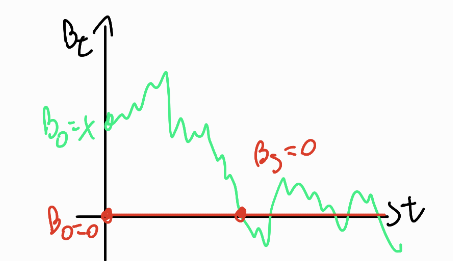
\includegraphics[width=0.5\linewidth]{img/screenshot020}
	\caption{Consider $B_s=0$, when the two paths coincide}
	\label{fig:screenshot020}
\end{figure}
Show that $X_{t}$ is Markov but it is not strong Markov. The heuristic intuition is that this is not strong Markov because to know the next step we must know whether we started from 0 or not. It is, though, Markov because the next move depends from a certain previous state. We cannot ``forget'' the origin.
\begin{definition}
	Let 
	\begin{equation*}
		\psi(x)=\ev{f(X_{t})|X_{0}=x}\qquad x\in\R
	\end{equation*}
	with $f$ being a function and $t>0$ fixed. We say that the process $X(t)$ has the \emph{Feller property} if
	\begin{equation}
		f\in C_{b}\implies \psi\in C_{b}\tag{\faProcedures}\label{procedure}
	\end{equation}
	where $C(b)$ is the space of continuous and bounded functions of $\R$.
\end{definition}
\begin{remark}
	The \bwm{} has the feller property:
	\begin{align*}
		\psi(x)&=\ev{f(B_{t})|B_{0}=x}\\
		&=\evs\Bigl[{f(\ubracketthin{B_{t}}_{\mathsf{N}(0,t)}+x)}\Bigr]\qquad\text{\small starting from $x$ means shifting}\\
		&=\int_{\R}f(x+y)\frac{1}{\sqrt{2\pi t}}e^{-\frac{y^{2}}{2t}}\dy
	\end{align*}
	and \ref{procedure} holds because since $f$ is continuous and bounded also the shifted function $f(x+y)$ is. The Gaussian density is smooth and integrates to 1.
\end{remark}
\begin{theorem}
	The \bwm{} is a strong Markov process with respect to its natural filtration.
\end{theorem}
\begin{remark}
	Strong Markov property can be rewritten as
	\begin{equation*}
		\ev{f(X_{T+h})|\F_{T}}=\ev{f(X_{h})|X_{0}=x}\Big|_{x=X_{T}}
	\end{equation*}
	for all stopping times $T$, all $h>0$ and all continuous bounded functions $f:\R\to\R$.
\end{remark}
\begin{fancyproof}
	\begin{enumerate}
		\item Consider the discrete stopping time $T_{n}$:
		\begin{align*}
			\ev{f(B_{T_{n}+h})|\F_{T_{n}}^{B}}&=\sum_{n}\indi_{\{T_{n}=n\}}\ev{f(B_{T_{n}+h})|\F_{n}^{B}}\quad\text{\tiny (conditioning all possibilities)}\\
			&\stackrel{\mathrm{markov}}{=}\sum_{n}\indi_{\{T_{n}=n\}}\ev{f(B_{T_{n}+g})|B_{n}}.
		\end{align*}
		But this means that, since there is only one term with $T_n=n$, at time $n$ the process restarts
		\begin{equation*}
			\sum_{n}\indi_{\{T_{n}=n\}}\ev{f(B_{h})|B_{0}=x}\Big|_{B_{T_{n}}=B_{n}=X}=\ev{f(B_{h})|B_{0}=x}\Big|_{B_{n}=x}.
		\end{equation*}
		The result works for $T_{n}$, so for discrete times we have the result.
		\item Now move to arbitrary stopping times. When we want to prove something about markoviality, we always start with discrete times and then move to continuous times. We know that for any stopping time $T$ there exists a sequence of decreasing stopping times $\{T_{n}\}$ converging to $T$:
		\begin{equation}
			\ev{f(B_{T_{n}+h})|\F^{B}_{T_{n}}}=\ev{f(B_{h})|B_{0}=x}\Big|_{x=B_{T_{n}}}\quad\text{for }\every n\geq1\tag{\faLandmark}\label{Landmark}.
		\end{equation}
		\begin{revise}
			Remember \emph{Hunt's lemma}: if $X_{n}\xrightarrow{n\to\infty}X$ a.s., $|X_{n}|\to Z$, $Z\in\lone$ and $\{\F_{n}\}$ is a filtration then
			\begin{equation*}
				\ev{X_{n}|\F_{n}}\to\ev{X|\F_{\infty}}\qquad\as{}
			\end{equation*}
			where $\F_{\infty}=\sigma\left(\bigcup_{n}\F_{n}\right)$.
		\end{revise}
		We take the limit of \ref{Landmark} for $n\to\infty$, then we apply Hunt's lemma to the left hand side and the Feller property to the right hand side:
		\begin{equation*}
			\ev{f(B_{\mathcolor{OliveDrab4}{T}+h})|\F_{\mathcolor{OliveDrab4}{T}}^{B}}=\ev{f(B_{h})|B_{0}=x}\Big|_{x=B_{\mathcolor{OliveDrab4}{T}}}.
		\end{equation*}
		This allows us to say that every Feller process is strong Markov!
	\end{enumerate}
\end{fancyproof}
\subsection{First passage times and Strong Markov Property}
As we have seen before, we can split the sample paths of a $\mathrm{BM}^{d}$ at a stopping time.
\begin{figure}[h]
	\centering
	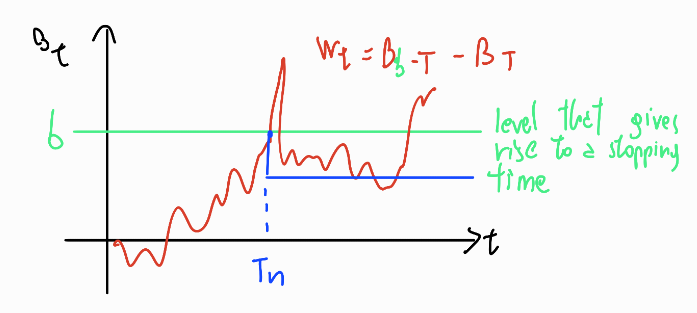
\includegraphics[width=0.7\linewidth]{img/screenshot021}
	\caption{More diagrams... are these even useful?}
	\label{fig:screenshot021}
\end{figure}
We are interested in knowing the distribution of the first passage time through b.
\begin{theorem}
	It holds
	\begin{equation*}
		\pr(\tau_{b}<t)=2\pr(B_{t.}\geq b)
	\end{equation*}
\end{theorem}
\begin{fancyproof}
	Assume $B_{t}$ attained $b$ at time $\tau_{b}$. Stop at $\tau_{b}$ and start a new \bwm{} $W_{s}$ from $B_{\tau_{b}}=b$
	\begin{align*}
		W_{s}+b&=\left(B_{\tau_{b}+s}-\ubracketthin{B_{\tau_{b}}}_{b}\right)+b\\
		&=B_{\tau_{b}+s}
	\end{align*}
	and this is again a BM but started at $b$. The probability of being above or below $b$ is the same, so
	\begin{align*}
		\pr(\tau_{b}\leq t,B_{t}<b)&=\pr\Big(\ubracketthin{\left\{\tau_{b}\leq t\right\}}_{\in\F^{B}_{\tau_{b}}}\cap\ubracketthin{\left\{B_{\tau_{b}+(t-\tau_{b})}-B_{\tau_{b}}<0\right\}}_{\in\F^{W}_{\infty}\independent\F^{B}_{\tau_{b}}}\Big)\\
		&=\pr(\tau_{b}\leq t)\ubracketthin{\pr\left(B_{\tau_{b}+(t-\tau_{b})}-B_{\tau_{b}}<0\right)}_{\unmezz\text{ because of symmetry around 0}}\\
		&=\unmezz\pr(\tau_{b}\leq t).
	\end{align*}
	Furthermore,
	\begin{align*}
		\pr(\tau_{b}\leq t)&=\pr(\tau_{b}\leq t, B_{t}\geq b)+\ubracketthin{\pr(\tau_{b}\leq t,B_{t}<b)}_{\unmezz\pr(\tau_{b}\leq t)}\\
		&\implies\unmezz\pr(\tau_{b}\leq t)=\pr(B_{t}\geq b)
	\end{align*}
\end{fancyproof}
	We can compute the probability density of $\tau_{b}$. We know
\begin{equation*}
	\pr(\tau_{b}\leq t)=2\int_{b}^{\infty}\frac{1}{\sqrt{2\pi t}}\exp\left\{-\frac{y^{2}}{2t}\right\}\dy
\end{equation*}
Hence if I take the derivative
\begin{align*}
	\frac{\dif}{\dt}&=\frac{b}{2\pi t^{3}}\exp\left\{-\frac{b^{2}}{2t}\right\}\\
	&=g(t)
\end{align*}
which is the probability distribution function of our first passage time. Now we can understand why the expectation of $t$ diverges. Consider
\begin{align}
	\ev{\tau_{b}}&=\int_{0}^{\infty}t\frac{b}{\sqrt{2\pi t^{3}}}\exp\left\{-\frac{b^{2}}{2t}\right\}\dt\nonumber\\
	&=\int_{0}^{\infty}\frac{b}{\sqrt{2\pi t}}\exp\left\{-\frac{b^{2}}{2t}\right\}\dt\nonumber\\
	&=\infty\label{hamsa}
\end{align}
so we have heavy tails!
\begin{figure}[H]
	\centering
	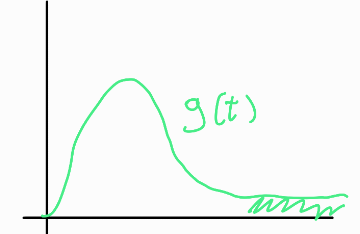
\includegraphics[width=0.5\linewidth]{img/screenshot022}
	\caption{Metal}
	\label{fig:screenshot022}
\end{figure}
There is a related property about this: let 
\begin{equation*}
	M_{t}:=\sup_{\vartheta\leq t}B_{\vartheta}
\end{equation*}
\begin{figure}
	\centering
	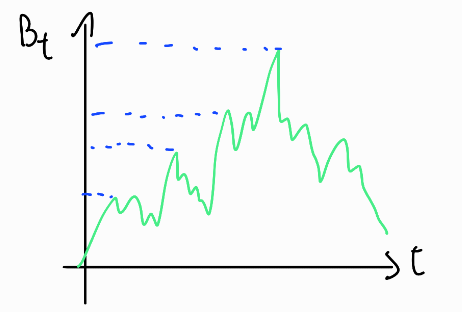
\includegraphics[width=0.7\linewidth]{img/screenshot023}
	\caption{As time $t$ evolves, its superior changes}
	\label{fig:screenshot023}
\end{figure}
It holds $$\pr(M_{t}\geq b)=2\pr(B_{t}\geq b)$$
\begin{fancyproof}
	Observe that 
	\begin{equation*}
		\{\tau_{b}\leq t\}=\{M_{t}\geq b\}.
	\end{equation*}
\end{fancyproof}
	$M_{t}$ and $|B_{t}|$ have the same distribution but what about their sample paths? We know that:
	\begin{itemize}
		\item $M_{t}$ is non decreasing;
		\item $|B_{t}|$ is not non decreasing.
	\end{itemize}
Their sample paths is very different!
\begin{remark}
	We have 
	\begin{equation*}
		M_{t}\sim M_{t}-B_{t}\quad\every y\geq 0 \qquad\text{given and fixed.}
	\end{equation*}
\end{remark}
\begin{fancyproof}
	By symmetry,\begin{align*}
		M_{t}\sim\sup_{s\leq t}(-B_{s})&=\sup_{s\leq t}((-B_{s}+B_{t})-B_{t})\\
		&=\sup_{s\leq t}\Big[\ubracketthin{(B_{t}-B_{t-s})-B_{s}}_{\claptext{$\widetilde{B}_{s}:$ time inversion symmetry}}\Big]\\
		&=\sup_{s\leq t}\widetilde{B}_{s}-B_{t}\sim M_{t}-B_{t}.
	\end{align*}
\end{fancyproof}
\subsection{First passage times for \bwm{} with drift}
Remember that for a \bwm{} the first passage time probability is 
\begin{equation*}
	\pr(\tau_{b}<t)=\frac{b}{\sqrt{2\pi t^{3}}}\expg{-\frac{b^{2}}{2t}}
\end{equation*}
And that $\pr(\tau_{b}<\infty)=1$.
For a process with strong Markov property (but not necessarily symmetry, like in the case of \bwm{} with drift) can we determine the distribution of the first passage time? This means looking for
\begin{equation*}
	\pr(\tau_{b}<t)=\pr\left(\tau_{b}<t|X(t_{0})=x_{0}\right).
\end{equation*}
Taking the derivative we get the probability density function of this distribution:
\begin{equation*}
	\frac{\dif}{\dt}\pr(\tau_{b}<t)=g_{\tau_{b}}({x_{0}})=...?
\end{equation*}
Aw hell nah. This is something we want to know for sure. 
This can apply to processes with continuous sample paths with strong Markov property (that is, diffusion processes). Think about \bwm{} with drift $X(t)=\sigma B_{t}+\mu t$, $\mu>0$, and its sample path:
\begin{figure}[H]
	\centering
	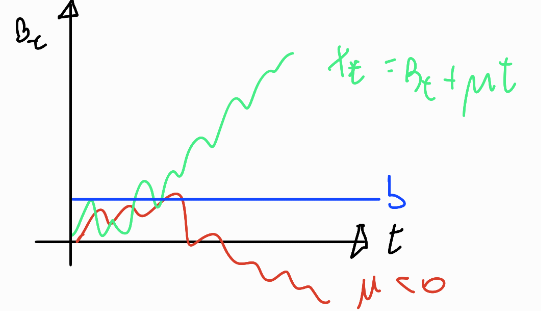
\includegraphics[width=0.5\linewidth]{img/screenshot024}
	\caption{This is the start of a downward spiral, believe me.}
	\label{fig:screenshot024}
\end{figure}
If the drift is positive and $b>0$ then we know that $\pr\left(\tau^{\mu}_{b}<\infty\right)=1$ because the process will incur in $b$ sooner or later. The focal point is that $X_{t}\geq B_{t}\as$, that is $X(t)$ \textit{dominates} $B_{t}$. On the other hand, if $\mu'<0$ then $\pr\left(\tau^{\mu'}_{b}<\infty\right)<1$ because the process will tend to escape from the bounds. It may happen that $b$ is reached, but in general it doesn't happen. Consider the probability that our process is above $b$ in figure \ref{fig:screenshot025}.
\begin{figure}[h]
	\centering
	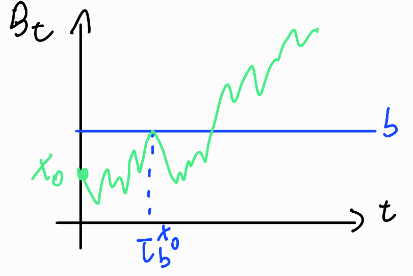
\includegraphics[width=0.5\linewidth]{img/screenshot025}
	\caption{$b$ is attained at $\tau_{b}^{x_0}$ after starting at $x_0$}
	\label{fig:screenshot025}
\end{figure}
Here we look for $\pr\left(\tau_{b}^{x_{0}}<t\right)$, that is the probability density function of $\tau_{b}^{x_{0}}$, \textit{the first passage time in $b$ with starting point $X(t_{0})=x_{0}$}.
This is like asking for the probability of $X(t)$ being greater than $x$, with $x>b$ and the process starting from $X(t_{0})=x_{0}$:
\begin{equation*}
	\pr\left(X(t)>x|X(t_{0})=x_{0}\right)\qquad x>b\tag*{\faSmile[regular]}\label{smile}.
\end{equation*}
Inverting the signs we can introduce the notation for a cumulative distribution function
\begin{equation*}
	\pr\left(X({t})<x|X(t_{0})=x_{0}\right)=F(x,t|x_{0},t_{0})
\end{equation*}
and therefore define the survival function
\begin{equation*}
		\pr\left(X(t)>x|X(t_{0})=x_{0}\right)=1-F(x,t|x_{0},t_{0})=\widebar{F}(x,t|x_{0},t_{0}).
\end{equation*}
Furthermore, consider $g_{b}^{x_{0}}(\tau)$, the probability of attaining $b$ at time $\tau$ with $X(t_0)=x_{0}$:
\begin{equation*}
	g_{b}^{x_{0}}(\tau)=g(b,\tau|X(t_{0})=x_{0}).
\end{equation*}
Note that this is a function of $\tau$ but it is characterized by the parameters $x_0$ (the starting point) and $b$ (the level we want to attain).
Now let's go back to the probability of $X(t)$ being above level $b$ (the one in equation \ref{smile}). We can rewrite it as
\begin{equation*}
	\ubracketthin{\pr\left(X({t})>x|X(t_{0})=x_{0}\right)}_{\widebar{F}(x,t|x_{0},t_{0})}=\ubracketthin{\int_{0}^{t}}_{\claptext{note the reversed integral}}\mathcolor{Gold3}{g_{b}^{x_{0}}(\tau)}\mathcolor{SpringGreen4}{\pr(X(t)>x|X(\tau)=b)}\dif\tau.
\end{equation*}
What we did here was using strong Markov property to ``split'' the probability between the \textcolor{Gold3}{probability of attaining $b$ starting from $x_0$} and \textcolor{SpringGreen4}{a new process that starts from $b$}, seeking the probability of transitioning from $b$ to $x$ in the remaning time! But this also means that
\begin{equation*}
	\widebar{F}(x,t|x_{0},t_{0})=\int_{0}^{t}g_{b}^{x_{0}}(\tau)\widebar{F}(x,t|\mathcolor{SpringGreen4}{b,\tau})\dif\tau.
\end{equation*}
Now derive with respect to $x$:
\begin{equation*}
	f(x,t|x_{0},t_{0})=\int_{0}^{t}\dif\tau g_{b}^{x_{0}}(\tau)f(x,t|b,\tau)\quad\text{for }x>b.
\end{equation*}
here $f(x,t|x_{0},t_{0})$ is simply the \emph{probability distribution function of the transition from $x_{0}$ to $x$ at time $t$}.\par
In 1943 Fortet\footnote{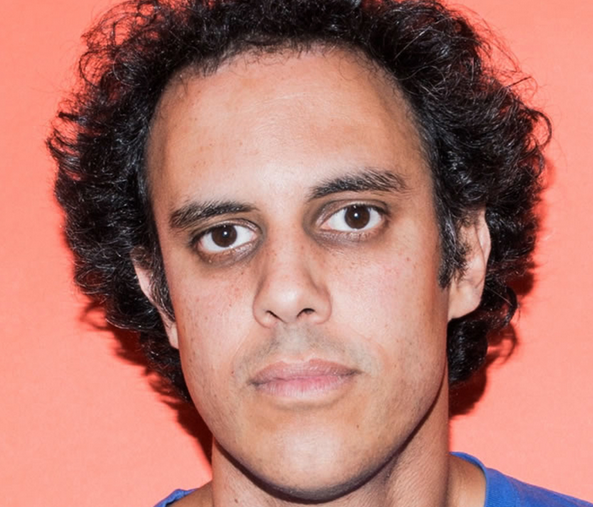
\includegraphics[width=0.1\linewidth]{img/screenshot026}
} proved that this equation holds also when $x=b$, introducing the so-called Fortet equation:
\begin{equation*}
	f(b,t|x_{0},t_{0})=\int_{0}^{t}\dif\tau g_{b}^{x_{0}}(\tau)f(b,t|b,\tau).\tag*{\faBarcode}\label{fortet}
\end{equation*}
In the \bwm{} with drift, we have that the process $X(t)=\sigma B(t)+\mu t$ is distributed as $\mathsf{N}\left(\mu(t-t_{0}),\sigma^{2}(t-t_{0})\right)$ and therefore our transition function is simply the normal distribution.
\begin{equation*}
	f(x,t|x_{0},t_{0})=\frac{\expg{-\frac{(x-x_0-\mu(t-t_{0}))^{2}}{2\sigma^{2}(t-t_{0})}}}{\sqrt{2\pi\sigma^{2}(t-t_{0})}}\tag*{\faCogs}\label{cogs}.
\end{equation*}
What we don't know is the function $g_{\tau_{b}}^{x_{0}}(t)$. Our problem now is solving a particular kind of equation called \emph{integral equations}. They are like differential equation, but with integrals. Pretty rad, if you ask me.\par
\begin{figure}[h]
	\centering
	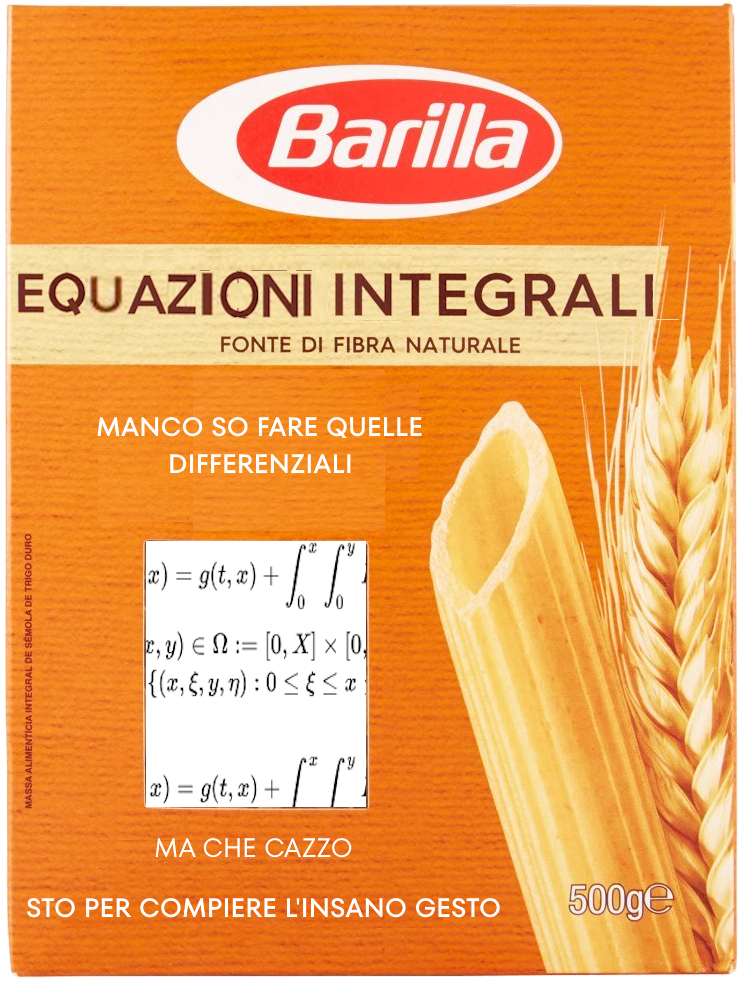
\includegraphics[width=0.4\linewidth]{img/integrali}
	\caption{Manco fa ridere 'sta troiata, ma l'ho fatta mentre aspettavo che la prof. caricasse gli appunti su Moodle. Cosa che non ha ancora fatto, tra l'altro.}
	\label{fig:integrali}
\end{figure}
We want to solve an equation of this form:
\begin{equation*}
	f(t)=\int_{0}^{t}\dif\tau K(t,\tau)y(\tau).
\end{equation*}
We call these ``Volterra integral equation of the first type''. In our case
\begin{equation*}
	\arraycolsep=1.4pt\def\arraystretch{2.2}
	\begin{array}{rlc}
		f(t)&=f(x,t|x_{0},t_{0})&\text{known \faCheck}\\
		K(t,\tau)&=f(b,t|b,\tau)&\text{known \faCheck}\\
		y(\tau)&=g_{{b}}^{x_{0}}(\tau)&\text{unknown \faExclamationTriangle}.
	\end{array}
\end{equation*}
This is an equation of the first type because the unknown is only in the integral. There exist also the second type Volterra equations:
\begin{equation*}
	f(t)=\varphi(y(t))+\int_{0}^{t}\dif\tau K(t,\tau)y(\tau)
\end{equation*}
but we leave these to more unhappy people than we are.
For time-homogeneous processes, we have
\begin{equation*}
	f(b,t|b,\tau)=f(b,t-\tau|b,0).
\end{equation*}
This is a simple consequence of stationarity of increments. Consider
\begin{equation*}
	f(b,t|x_{0},t_{0})=\int_{0}^{t}\dif\tau g_{b}^{x_{0}}(\tau)f(b,t-\tau|b,0).\tag*{\faCat}\label{cat}
\end{equation*} We can see, though, that the integral \ref{cat} is a convolution.
\begin{revise}
	You don't know remember what a convolution is, you poor wretched bastard who studied economics as undergrad? The convolution of two functions $f(t)$ and $g(t)$ is given by
	\begin{equation*}
		(f\ast g)(t)=\int_{0}^{t}f(\tau)g(t-\tau)\dif\tau.
	\end{equation*}
\begin{figure}[H]
	\centering
	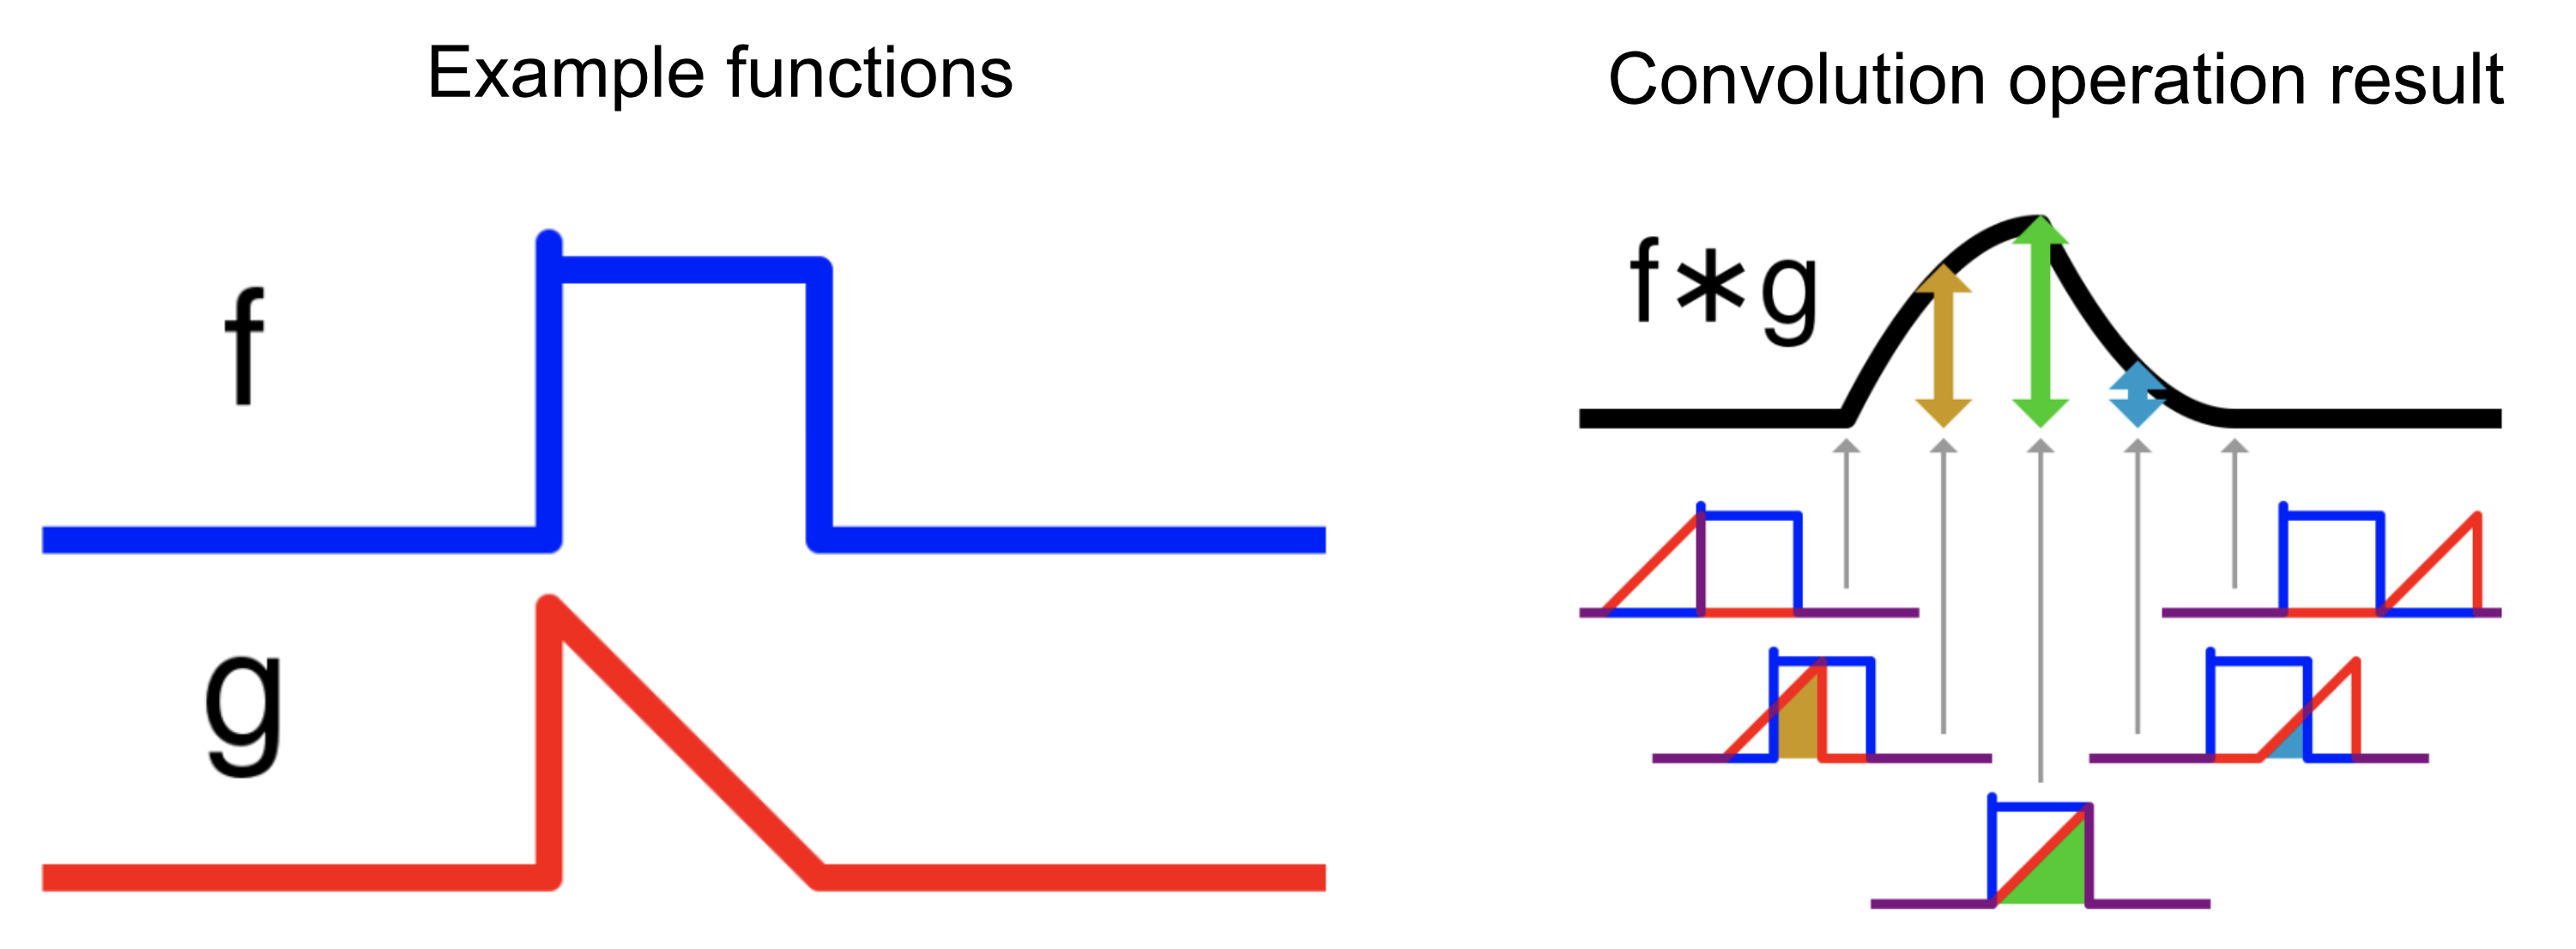
\includegraphics[width=0.5\linewidth]{img/screenshot027}
	\caption{This image has always been helpful to me. I just love it.}
	\label{fig:screenshot027}
\end{figure}
Convolutions have nice properties. For example, we can easily turn them into simple multiplications using Laplace transforms. The Laplace transform of a function is defined as 
\begin{equation*}
	\mathcal{L}\{f(t)\}(\lambda)=\mathcal{L}_{\lambda}\{f(t)\}=\int_{0}^{\infty}e^{-\lambda t}f(t)\dt\qquad\text{with }\lambda=\sigma+i\omega.
\end{equation*}
Here $\sigma$ introduces a decaying/growing component while $i\omega$ introduces the oscillatory component, just like Fourier transforms! Indeed, Fourier transforms lack the ``$\sigma$'' part, only relying on the ``spinning'' part of the signal. While Fourier transform lets us go from the time domain to the frequency domain, Laplace transform lets us go to the \textit{complex frequency domain}. This is why this bad boy Laplace transform is also well suited to represent signals/functions that are not periodic. This is bananas, very cool!\par
Anyway, back to our matter: Laplace transforms can make our life easier with convolutions. This is because
\begin{equation*}
	\laplace{(f\ast g)(t)}=\laplace{f(t)}\cdot\laplace{g(t)}.
\end{equation*}
This is much more manageable! Just remember to do the inverse transform after to go back to your original domain. This can be tricky, because the inverse Laplace transform depends on the form of the transformed function. We often have to use tables of known Laplace transforms or other extravagant techniques that I will not delve into.
\end{revise}
As we said, it's pretty standard to use Laplace transforms to deal with convolutions. We could also use Fourier transforms, but we are cooler than that. So transform \ref{fortet} into our new equation:
\begin{equation*}
	\begin{array}{c}
			f(b,t|x_{0},t_{0})=\int_{0}^{t}\dif\tau g_{b}^{x_{0}}(\tau)f(b,t-\tau|b,0)=\int_{0}^{t}\dif\tau g_{b}^{x_{0}}(\tau)f(b,t|b,\tau)\\[-0.4pt]
			\Downarrow\\[-1pt]
			\laplace{f(b,t|x_{0},t_{0})}=\laplace{g_{b}^{x_{0}}(\tau)}\cdot\laplace{f(b,t|b,\tau)}.
	\end{array}
\end{equation*}
We know that 
\begin{align*}
	\laplace{f(b,t|x_{0},t_{0})}&=f_{\lambda}(b|x_{0})\\
	\laplace{f(b,t|b,\tau)}&=f_{\lambda}(b|b)\\
	\laplace{g_{b}^{x_{0}}(\tau)}&=g_{\lambda}(b|x_{0}).
\end{align*}
Note that these equations do not show $t$ anymore because they don't live in the time domain anymore, but in the complex frequency domain. $t$ ``becomes'' $\lambda$ (intuitively). Same goes for $g_{b}^{x_{0}}(\tau)$, where $\tau$ gets ``integrated out'' leaving behind the parameters $b$ and $x_{0}$. So we get
\begin{equation*}
	f_{\lambda}(b|x_{0})=g_{\lambda}(b|x_{0})\cdot f_{\lambda}(b|b)\implies g_{\lambda}(b|x_{0})=\frac{f_{\lambda}(b|x_{0})}{f_{\lambda}(b|b)}.
\end{equation*}
Let's take the only example we can apply in this stage of our life: the \bwm{} with drift (and $\sigma^{2}=1$). Apply the Laplace transform to \ref{cogs} (setting $t_0=0$) and get: 
\begin{align*}
	f_{\lambda}(b|x_{0})&=\int_{0}^{\infty}e^{-\lambda t}\frac{1}{\sqrt{2\pi t}}\expg{-\frac{(b-\mu t-x_{0})^{2}}{2t}}\dt\\
	&=\frac{e^{\mu(b-x_{0})}e^{-\sqrt{\mu^{2}+2\lambda}(b-x_{0})}}{\sqrt{2\lambda+\mu^{2}}}
\end{align*}
and
\begin{align*}
	f_{\lambda}(b|b)&=\int_{0}^{\infty}e^{-\lambda t}\frac{1}{\sqrt{2\pi t}}\expg{-\frac{\mu^{2}t}{2}}\dt\\
	&=\frac{1}{\sqrt{2\lambda+\mu^{2}}}.
\end{align*}
It becomes now quite easy to compute $g_{\lambda}(b|x_{0})$:
\begin{align*}
	g_{\lambda}(b|x_{0})&=\frac{e^{\mu(b-x_{0})}e^{-\sqrt{\mu^{2}+2\lambda}(b-x_{0})}}{\cancel{\sqrt{2\lambda+\mu^{2}}}}\cdot\cancel{\sqrt{2\lambda+\mu^{2}}}\\
	&=e^{\mu(b-x_{0})}e^{-\sqrt{\mu^{2}+2\lambda}(b-x_{0})}.
\end{align*}
We are lucky: for this function we can analytically compute the inverse Laplace transform.
\begin{equation*}
	g(b,t|x_{0})=\frac{|b-x_{0}|}{\sqrt{2\pi t^{3}}}\expg{-\frac{(b-x_{0}-\mu t)^{2}}{2t}}.
\end{equation*}
This is our function $g_{b}^{x_{0}}(\tau)$ expressed in the time domain! This is a good first result, but there is more to it. Consider the Laplace transform evaluated at $\lambda=0$: this is like summing over all time without the decay, since when $\lambda=0$ we are essentially removing the exponential decay factor from the integral. In this case the fact that $e^{-\lambda t}=1$ gives us the \textit{total probability} of the event occurring with finite time.
\begin{align*}
	g_{\lambda}(b|x_{0})\big|_{\lambda=0}&=\int_{0}^{\infty}e^{-\lambda t}g(b,t|x_{0},t_{0})\dt\big|_{\lambda=0}\\
	&=\int_{0}^{\infty}g(b,t|x_{0},t_{0})\\
	&=\pr\left(\tau_{b}^{x_{0}}<\infty\right).
\end{align*}
Since 
\begin{equation*}
	g_{\lambda}(b|x_{0})=e^{\mu(b-x_{0})}e^{-\sqrt{\mu^{2}+2\lambda}(b-x_{0})}
\end{equation*}
we have that
\begin{equation*}
		g_{\lambda}(b|x_{0})\big|_{\lambda=0}\begin{cases}
			1&\mu\geq0\\
			e^{-2|\mu|(b-x_{0})}&\mu<0.
		\end{cases}
\end{equation*}
This is our second result and it tells us that, as a function of $\mu$, the distribution of the first hitting time in a finite time has a decaying probability of reaching $b$ (as $b$ gets away from the starting point $x_{0}$) and then it degenerates to 1. But hold tight, there is MORE! Consider
\begin{align*}
	\frac{\dif g_{\lambda}}{\dif\lambda}\Big|_{\lambda=0}&=\frac{\dif}{\dif\lambda}\int_{0}^{\infty}\dif te^{-\lambda t}g_{b}^{x_{0}}(t)\big|_{\lambda=0}\\
	&=\int_{0}^{\infty}(-t)e^{-\lambda t}g_{b}^{x_{0}}(t)\dt\big|_{\lambda=0}\\
	&=-\ev{\tau^{x_{0}}_{b}}
\end{align*}
and
\begin{equation*}
	\frac{\dif^{n} g_{\lambda}}{\dif\lambda^{n}}\Big|_{\lambda=0}=(-1)^{n}\ev{\left(\tau_{b}^{x_{0}}\right)^{n}}
\end{equation*}
So we can compute moments from the Laplace transform! For the \bwm{} with drift $\mu>0$ (for $\mu<0$ it doesn't make sense to compute the moments) we have
\begin{align*}
	-\frac{\dif}{\dif\lambda}e^{\left(\mu-\sqrt{\mu^{2}+2\lambda}\right)(b-x_{0})}\Big|_{\lambda=0}&=\frac{b-x_{0}}{\sqrt{\mu^{2}+2\lambda}}e^{\left(\mu-\sqrt{\mu^{2}+2\lambda}\right)(b-x_{0})}\Big|_{\lambda=0}\\
	&=\frac{b-x_{0}}{\mu}=\ev{\tau_{b}^{x_{0}}}
\end{align*}
So the expectation is not only finite, but it also tends to be small since it depends inversely on the drift and directly on the distance between $b$ and $x_{0}$. The crossing time exists, but remember how in normal \bwm{} this time was infinite (see \ref{hamsa})? This is the proof that the drift helps attaining $b$!\par
Consider the case $b<x_{0}$:
\begin{figure}[H]
	\centering
	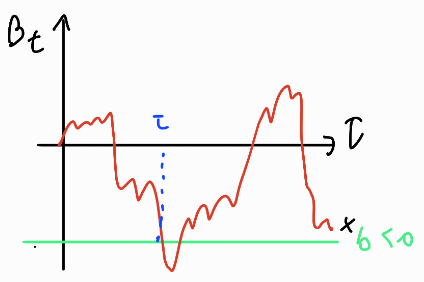
\includegraphics[width=0.4\linewidth]{img/screenshot028}
	\caption{This hellish part is almost over... but you gotta admit it was pretty cool, in a sense. Maybe I am just losing my mind.}
	\label{fig:screenshot028}
\end{figure}
We know that 
\begin{equation*}
	\begin{array}{c}
		\pr(X(t)<x|X(t_{0})=x_{0})=\int_{0}^{t}g_{b}^{x_{0}}(\tau)\pr(X(t)<x|X(t)=b)\dif\tau\\
		\Downarrow\\
		F(x,t|x_{0})=\int_{0}^{t}g_{b}^{x_{0}}(\tau)F(x,t|b,\tau)\dif\tau
	\end{array}
\end{equation*}
Which is exactly the Fortet equation. So everything we said before applies to this case as well.\par
And what's the deal with time-dependent boundaries?
\begin{figure}[H]
	\centering
	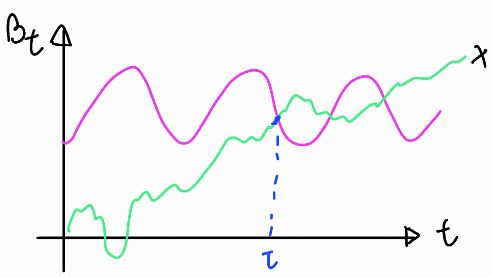
\includegraphics[width=0.5\linewidth]{img/screenshot029}
	\caption{And what's the deal with airplane food?}
	\label{fig:screenshot029}
\end{figure}
We should understand that the probability of $\tau$ is not affected.
\begin{equation*}
	\begin{array}{c}
		\pr(X(t)>x|X(t_{0})=x_0)=\int_{0}^{t}\dif\tau g(\mathcolor{OliveDrab4}{b(\tau)},t|x_{0})\cdot\pr(X(t)>x|\mathcolor{OliveDrab4}{b(\tau)},\tau)\\
		\Downarrow\\
		f(b(t),t|x_{0})=\int_{0}^{t}\dif\tau g(b(\tau),\tau|x_{0})f(b(t),t|b(\tau),\tau).
	\end{array}
\end{equation*}
This is still the Fortet equation. I would have never guessed that that guy was not only capable of doing terrible Skrillex and Fred Again featurings but also well versed in stochastic processes.\par
Up to now, we worked having the process (meaning its probability density function) and the shape of the boundary. But what if we are in the inverse situation? What if we have the process and the first passage time distribution and \textit{we want to determine the boundary shape}? Heh.
\section{Useful laws about \bwm's path}
\subsection{Reflection principle}
The \emph{reflection principle} is the property according to which, if a path of a \bwm{} attains a level $b$ at time $s$, the subsequent path has the same probability as its reflected path.
\begin{figure}[h]
	\centering
	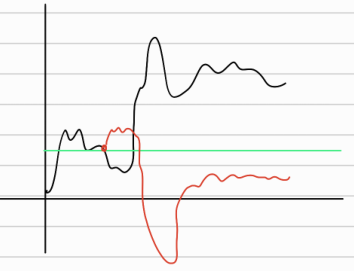
\includegraphics[width=0.4\linewidth]{img/screenshot030}
	\caption{When I exported my notes I forgot to remove the page lines...}
	\label{fig:screenshot030}
\end{figure}
There is an alternative definition.
\begin{definition}
	The reflected sample path of a \bwm{} after a stopping time $\tau(\omega)$ is defined as
	\begin{equation*}
		W(t,\omega):=\begin{cases}
			B(t,\omega)&0<t<\tau(\omega)<\infty\\
			2B(\tau(\omega),\omega)-B(t,\omega)&\tau(\omega)<t<\infty.
		\end{cases}
	\end{equation*}
\end{definition}
We can see how $	2B(\tau(\omega),\omega)-B(t,\omega)$ is simply the mirrored sample path obtained by $B_{\tau}-\left(B_{t}-B_{\tau}\right)$: after $\tau$ we have the same increment but with opposite sign.
\begin{theorem}
	\emph{Levy's triple law 1948}: Let $B={(B_{t})}_{t\geq0}$ be a standard BM. Then, if
	\begin{equation*}
		m_{t}=\inf_{s\leq t}B_{s}\qquad M_{t}=\sup_{s\leq t}B_{s},
	\end{equation*} the probability
	\begin{equation*}
		\pr(m_{t}>a,M_{t}<b,B_{t}\in\dx)\tag*{\faChalkboard}\label{chalk}
	\end{equation*}
	is equal to
	\begin{equation*}
		\frac{\dx}{\sqrt{2\pi t}}\sum_{n=-\infty}^{+\infty}\left[\expg{-\frac{x+2n(b-a)^{2}}{2t}}-\expg{-\frac{x-2a-2n(b-a)^{2}}{2t}}\right].
	\end{equation*}
\end{theorem} 
\begin{figure}[h]
	\centering
	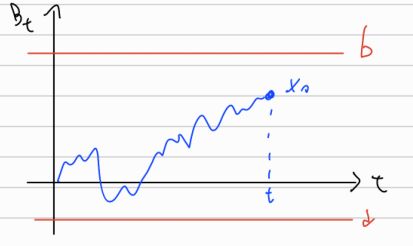
\includegraphics[width=0.5\linewidth]{img/screenshot031}
	\caption{We are looking for the probability of the \bwm{} to be between $a$ and $b$.}
	\label{fig:screenshot031}
\end{figure}
We get an infinite summation with two terms: the first one represent the ``normal'' path, while the other one represents the mirrored path reflected at $a$. We don't do the whole the proof\footnote{Yippie!!} because that would take like two pages of useless calculations and we don't want that. We just give a sketch of the proof:
\begin{fancyproof}
	Let 
	\begin{equation*}
		\tau=\inf\left\{t\geq0:B_{t}\notin(a,b)\right\}
	\end{equation*}
	be the first exit time from $a,b$. We have that 
	\begin{align*}
		\pr(m_{t}>a,M_{t},B_{t}\in k)&=\pr(\tau>t,B_{t}\in K)\\
		&=\pr(B_{t}\in K)-\pr(\tau\leq t,B_{t}\in K)\\
		&=\pr(B_{t}\in K)-\pr(B_{\tau}=a,\tau\leq t,B_{t}\in K)-\\
		&-\pr(B_{\tau}=b,\tau\leq t,B_{t}\in K).
	\end{align*}
	Introduce the reflection operator:
	\begin{equation*}
		\begin{array}{c}
			\mathfrak{R}_{a}x=2a-x\\
			\mathfrak{R}_{b}x=2b-x.
		\end{array}
	\end{equation*}
	Note that, using the reflection principle,
	\begin{align*}
		\pr(B_{\tau}=a,\tau\leq t,B_{t}\in K)&=\pr(B_{\tau}=a,\tau\leq t,B_{t}\in\mathfrak{R}_{a}K)\\
		&=\pr(B_{\tau}=a,B_{t}\in\mathfrak{R}_{a}K)\\
		&=\pr(B_{t}\in\mathfrak{R}_{a}K)-\pr(B_{\tau}=b,B_{t}\in\mathfrak{R}_{a}K)\\
		&=\pr(B_{t}\in\mathfrak{R}_{a}K)-\pr(B_{\tau}=b,B_{t}\in\mathfrak{R}_{b}\mathfrak{R}_{a}K)\\
		&=\pr(B_{t}\in\mathfrak{R}_{a}K)-\pr(B_{t}\in\mathfrak{R}_{b}\mathfrak{R}_{a}K)+\\
		&+\pr(B_{\tau}=a,B_{t}\in\mathfrak{R}_{n}\mathfrak{R}_{a}K)\\
		&\ldots
	\end{align*}
	The idea is that we keep on rewriting the probabilities as their marginals minus (or plus) something until we arrive to our summation.
\end{fancyproof}
We know that
\begin{equation*}
	M_{t}=\sup_{\vartheta\leq t}B_{\vartheta}=\sup_{\vartheta\leq t}(-B_{\vartheta})=\sup_{\vartheta\leq t}\big[\ubracketthin{-B_{\theta}+B_{t}}_{B_{t}-B_{\vartheta}\sim\widetilde{B}_{\vartheta}}-B_{t}\big]\sim\sup_{\vartheta\leq t}\left[\widetilde{B}_{\vartheta}-B_{t}\right]\sim M_{t}-B_{t}.
\end{equation*}
So... $M_{t}\sim M_{t}-B_{t}$? Are we going crazy yet?
\begin{theorem}
	Consider a $\mathrm{BM}^d$ with $b\in\R$. Let
			\begin{equation*}
			m_{t}=\inf_{s\leq t}B_{s}\qquad M_{t}=\sup_{s\leq t}B_{s}
	\end{equation*}
and
\begin{equation*}
	\tau_{b}:=\inf\left\{t\geq0:B_{t}=b\right\}.
\end{equation*}
Then
\begin{align*}
	M_{t}&\sim\underset{\circled{1}}{|B_{t}|}\sim\underset{\circled{2}}{-m_{t}}\sim\underset{\circled{3}}{M_{t}-B_{t}}\sim\underset{\circled{4}}{B_{t}-m_{t}}\\
	&\sim\underset{\circled{5}}{\frac{\sqrt{2}}{\sqrt{\pi t}}e^{-\frac{x^{2}}{2t}}\dx}
\end{align*}
and 
\begin{equation*}
	\tau_{b}\sim\frac{|b|}{\sqrt{2\pi t^{3}}}\expg{-\frac{b^{2}}{2t}}.
\end{equation*}
\end{theorem}
\begin{fancyproof}
	\begin{enumerate}[\circnum]
		\item\label{triple1} Already proven.
		\item\label{triple2} This is left as an exercise: we need to prove that 
		\begin{equation*}
			m_{t}=\inf_{s<t}B_{s}=-\sup_{s\leq t}(-B_{s})=-t.
		\end{equation*}
		\item\label{triple3} Rethink this as
		\begin{equation*}
			M_{t}-B_{t}=\sup_{s\leq t}(B_{s}-B_{t})=\sup_{s\leq t}(B_{t-s}-B_{t})\sim\sup_{s\leq t}B_{s}=M_{t}.
		\end{equation*}
		\begin{remark}
			we know that $M_{t}\sim|B_{t}|$ (we proved it), so 
			\begin{equation*}
				M_{t}-B_{t}\sim|B_{t}|-B_{t}\sim|B_{t}|\sum M_{t}.
			\end{equation*}
		\end{remark}
		\item\label{triple4} This follows from combining \ref{triple3} with symmetry.
	\end{enumerate}
\end{fancyproof}
\subsection{Arcsin laws}
Consider a \bwm{} in the interval ($0,t$). We want to study the last 0 before $t$, that is
\begin{equation*}
	\xi_{t}:=\sup\left\{s\leq t:B_{s}=0\right\}.
\end{equation*}
\begin{figure}[h]
	\centering
	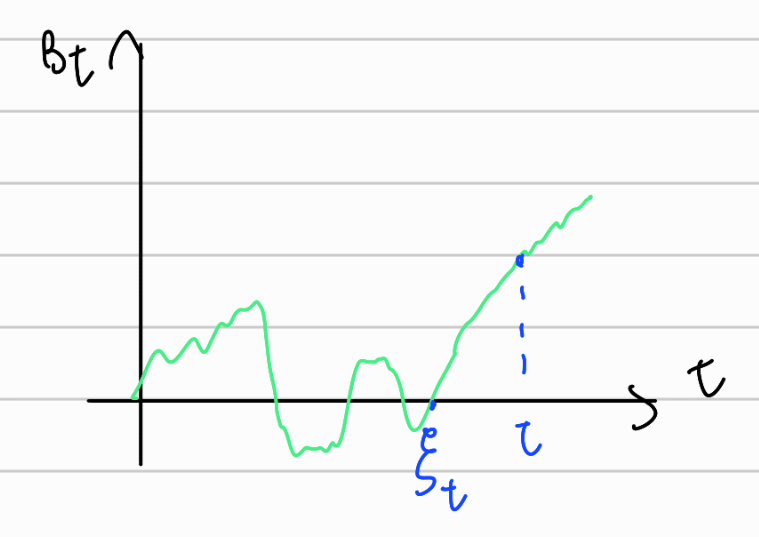
\includegraphics[width=0.5\linewidth]{img/screenshot032}
	\caption{I am not sure the sup gets defined in this way...}
	\label{fig:screenshot032}
\end{figure}
Of course this is not a stopping time because to assess whether a 0 is the last 0 before $t$ we need to peek into the future.
\begin{theorem}
\emph{Arcsin law I}.	Let ${(B_{t})}_{t\geq0}$ be a one-dimensional \bwm{} and let $\xi_{t}$ be the largest zero of $B_{s}$ in $[0,t]$. Then for $\every 0<s<t$ we have
	\begin{equation*}
		\pr(\xi_{t}<s)=\frac{2}{\pi}\arcsin\sqrt{\frac{s}{t}}.
	\end{equation*}
\end{theorem}
\begin{fancyproof}
	Take
	\begin{align*}
		h(s)&=\pr(B_{u}\neq 0,\every u\in[s,t])\\
		\text{\scriptsize conditioning the $\pr$ to the value of $B$ at $s\rightarrow$}&=\int_{\R}\pr^{B_{s(\omega)}}(B_{u-s},\every u\in[s,t])\cdot\pr(B_{s\in\dif b})\\
	\end{align*}
	So my process at time $s$ will be in $B_{s}(\omega)=b$. I can write the probability conditioned to being in $b$ as $\pr^{b}$. What the fuck is this horrid notation now?
	\begin{align*}
		\int_{\R}\pr^{B_{s(\omega)}}(B_{u-s},\every u\in[s,t])\cdot\pr(B_{s\in\dif b})&=\int_{\R}\pr^{b}(B_{u-s}\neq0,\every u\in[s,t])f_{B_{s}}(b)\dif b\\
		&=\int_{\R}\pr^{0}(B_{u-s}\neq-b,\every u\in[s,t])f_{B_{s}}\tag*{\faCocktail}\label{cock}\\
		&=\int_{\R}\pr^{0}(B_{v}\neq-b,\every v\in[0,t-s])f_{B_{s}}(b)\dif b\\
		&=\int_{\R}\pr^{0}(\tau_{-b}>t-s)\ubracketthin{f_{B_{s}}(b)}_{\mathclap{\frac{1}{\sqrt{2\pi s}}e^{-\frac{b^{2}}{2s}}}}\dif b.
	\end{align*}
	Note that
	\begin{equation*}
		\pr^{0}(\tau_{b}\geq t-2)=2\sqrt{\frac{1}{2\pi(t-s)}}\int_{0}^{b}e^{-\frac{x^{2}}{2(t-2)}}\dx
	\end{equation*}
	so
	\begin{equation*}
		\eqref{cock}=2\int_{0}^{\infty}\left(\sqrt{\frac{1}{2\pi(t-s)}}\int_{0}^{b}e^{-\frac{x^{2}}{2(t-2)}}\dx\right)\cdot\frac{1}{\sqrt{2\pi s}}\cdot e^{-\frac{b^{2}}{2s}}\dif b.
	\end{equation*}
	So, calling $\beta=\frac{b}{\sqrt{s}}$ and $\mu=\frac{x}{\sqrt{t-s}}$, we get
	\begin{equation*}
		h(s)=\frac{2}{\pi}\int_{0}^{\infty}\left(\int_{0}^{\beta\sqrt{\frac{s}{t-s}}}e^{-\frac{u^{2}}{2}\du}\right)e^{-\frac{\beta^{2}}{2}}\dif\beta.
	\end{equation*}
	Why do we have to endure suffering? Consider
	\begin{equation*}
		h'(s)=\frac{1}{\pi}\frac{1}{\sqrt{s(t-s)}}\qquad0\leq s\leq t.
	\end{equation*}
	\begin{revise}
		Remember that 
		\begin{equation*}
			\frac{\dif}{\ds}\arcsin\sqrt{\frac{s}{t}} =\frac{\pi}{2}h'(s).
		\end{equation*}
	\end{revise}
	So
	\begin{equation*}
		h(s)=\mathcolor{OliveDrab4}{\frac{2}{\pi}\arcsin\sqrt{\frac{s}{t}}}=1-\frac{2}{\pi}\arccos\sqrt{\frac{s}{t}}\quad s\leq t.
	\end{equation*}
\end{fancyproof}
\begin{insult}
	Trigonometric equations?? In MY fucking measure theory notes? 
\end{insult}
\begin{remark}
	The density is $$\pr(\xi\in\ds)=\frac{1}{\pi}\frac{1}{\sqrt{s(t-s)}}.$$
	If we choose $t=1$ we get 
	\begin{equation*}
		\pr(\xi\in\ds)=\frac{1}{\pi}s^{-\sfrac{1}{2}}(1-s)^{\sfrac{1}{2}}.
	\end{equation*}
	This is a Beta distributions with parameters $(\sfrac{1}{2},\sfrac{1}{2})$.
\end{remark}
\begin{figure}[h]
	\centering
	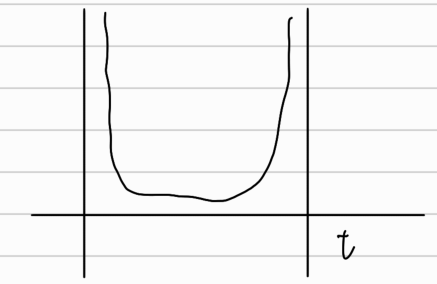
\includegraphics[width=0.5\linewidth]{img/screenshot033}
	\caption{You will take this distribution and you WILL like it.}
	\label{fig:screenshot033}
\end{figure}
The shape is symmetric: there is a high probability of values at the extreme of the interval, so it is highly probable that all the values ar either at 0 or at $t$.
\begin{figure}[h]
	\centering
	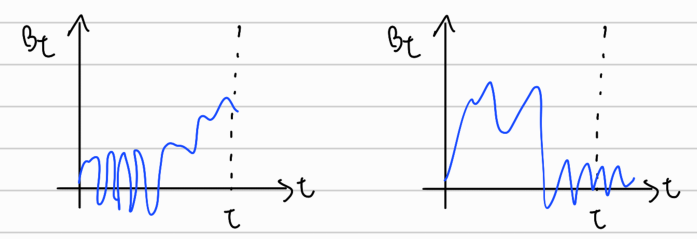
\includegraphics[width=0.6\linewidth]{img/screenshot034}
	\caption{I am not entirely sure bout there graphs, but I think they are correct.}
	\label{fig:screenshot034}
\end{figure}
\begin{remark}
	We can read the law in an alternative way. Recall that 
	\begin{equation*}
		X_{t}=M_{t}-B_{t}
	\end{equation*}
	has the same law as $B_{t}$. Then observe that:
	\begin{itemize}
		\item zeroes of $B_{t}$ coincide with zeroes of $|B_{t}|$;
		\item the last zero of $X_{t}$ has the same distribution as the last zero of $B_{t}$;
		\item the last zero of $X_{t}$ happens when $B_{t}$ attains its supremum.
	\end{itemize}
	This means that (and this is \emph{arcsin law III})
	\begin{equation*}
		\pr(\ubracketthin{M}_{\claptext{time of last maximum}}<X)=\frac{2}{\pi}\arcsin\sqrt{x}.
	\end{equation*}
\end{remark}
What about the \emph{arcsin law II}? Consider a \bwm{} $(B_{t})$ and
\begin{equation*}
	G_{t}:=\int_{0}^{t}\indi_{(0,\infty)}(B_{s})\ds.
\end{equation*}
$G_{t}$ is the time that the process spends above the level 0. We have that 
\begin{equation*}
	\pr(G_{t}\leq x)=\frac{2}{\pi}\arcsin\sqrt{\frac{x}{t}}\qquad x\in[0,t].
\end{equation*}
Again, small and large times are more probable. There is another arcsin law (I call it \emph{arcsin law IV}).
\begin{figure}[h]
	\centering
	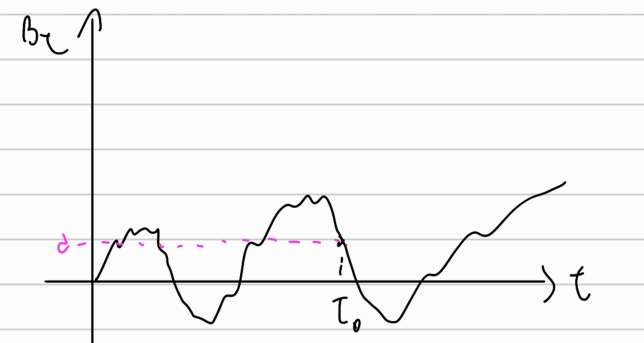
\includegraphics[width=0.5\linewidth]{img/screenshot035}
	\caption{What is $a$? We will never know!}
	\label{fig:screenshot035}
\end{figure}
We want the probability $\alpha$ that $B_{t}$ has at least one $0$ in $[t_{0},t]$.
\begin{equation*}
	\alpha=\frac{2}{\pi}\arccos\sqrt{\frac{t_{0}}{t}}.
\end{equation*}
So we are learning about how the process behaves either at the origin or far away from it.
\begin{fancyproof}                                                                      
	\begin{align*}                                                                         
		\beta&=\pr(\text{$B_{t}$ has at least one zero in }[t_{0}, t_{1}]|B_{t_{0}}=a)\\      
		&=\pr(\tau_{a}\leq t_{1}-t_{0})\\                                                     
		&=\frac{|a|}{\sqrt{2\pi}}\int_{0}^{t_{1}-t_{0}}\frac{e^{-\frac{a^{2}}{2u}}}{\sqrt{u^{3}}}\du
	\end{align*}                                                                           
	and                                                                                    
	\begin{align*}                           
		\alpha&=\int_{0}^{\infty}\dif a\beta\pr(|B_{t_{0}}|\in(a,a+\dif a)|B_{0}=a)\\         
		&=\int_{0}^{\infty}\left(\frac{s}{\sqrt{2\pi}}\int_{0}^{t_{1}-t_{0}}\frac{e^{-\frac{a^{2}}{2u}}}{\sqrt{u^{3}}}\du\right)\sqrt{\frac{2}{\pi t_{0}}}e^{-\frac{a^{2}}{2t}}\dif a\\
		&=\ldots=\frac{2}{\pi}\arccos\sqrt{\frac{t_{0}}{t}}.
	\end{align*}
\end{fancyproof}
Truly horrible. Here is a cheatsheet:
\begin{center}
			\begin{tabular}{|c|c|}
				\hline
	\emph{Arcsin law I}&\emph{Arcsin law II}\\
	\hline
	$\pr(\xi_{t}<s)=\frac{2}{\pi}\arcsin\sqrt{\frac{s}{t}}$&$\pr(G_{t}\leq x)=\frac{2}{\pi}\arcsin\sqrt{\frac{x}{t}}$\\
	\hline
	\emph{Arcsin law III}&\emph{Arcsin law IV}\\
	\hline
	$\pr({M}<X)=\frac{2}{\pi}\arcsin\sqrt{x}$&$\alpha=\frac{2}{\pi}\arccos\sqrt{\frac{t_{0}}{t}}$\\
	\hline
\end{tabular}
\end{center}
\section*{Exercises}
\label{sec:exer3}
\addcontentsline{toc}{section}{\nameref{sec:exer3}}
\begin{exercise}
	Let $B(t)$ be a \bwm{} and let $0<s\leq t\leq u\leq v$.
	\begin{enumerate}
		\item Show that the \rv s $\frac{1}{t}B(t)\frac{1}{s}B(s)$ and $aB(u)+bB(v)$ are independent for any $a,b\in\R$.
		\item Show that the random variables $aB(s)+bB(t)$ and $\frac{1}{v}B(v)\frac{1}{u}B(u)$ are independent for any $a,b\in\R$ satisfying the condition $as+bt=0$.
	\end{enumerate}
\end{exercise}
\begin{exercise}
	Let $X(t)$ be a one-dimensional \bwm{} with drift $\mu$ and let $T=\inf\left\{t\geq0:X(t)>b\right\}$ be its first passage time from a boundary $b>0$.
	\begin{enumerate}
		\item Using the Fortet equation determine when
		\begin{equation*}
			\pr(T\leq\infty)=1.
		\end{equation*}
		\item Determine the distribution of $T$. Hint: make use of Laplace transforms, their expression is reported in the additional material uploaded on Moodle.
		\item Determine $\ev{T}$.
	\end{enumerate}
\end{exercise}
\begin{exercise}
	Let $B(t)$ be a one dimensional \bwm{} and let $T_{i}=\inf\{t\geq 0: B(t)>i\}$, $i=-1,1,2$. Determine 
	\begin{equation*}
		\pr(T_{1}<T_{-1}<T_{s}).
	\end{equation*}
\end{exercise}
\begin{exercise}
	Consider a one dimensional \bwm. Let
	\begin{itemize}
		\item $\tau_{b}:=\inf\{t>0:B(t)\geq b\}$;
		\item $\tau_{-b}:=\inf\{t>0:B(t)\leq -b\}$;
		\item $\tau_{cb}:=\inf\{t>0:B(t)\geq cb\}$.
	\end{itemize}
	Prove that
	\begin{enumerate}
		\item $\tau_{b}\sim\tau_{-b}$;
		\item $\tau_{cb}\sim c^{2}\tau_{b}$.
	\end{enumerate}
\end{exercise}
\subsection{Brownian bridge}
\begin{definition}
	Let ${(B_{t})}_{t\geq 0}$ be a one-dimensional \bwm{}. Then $B$ conditioned on $B_{0}=B_{1}=0$ (or $B_{0}=B_{t}=0$ with $t$ fixed).
\end{definition}
\begin{figure}[h]
	\centering
	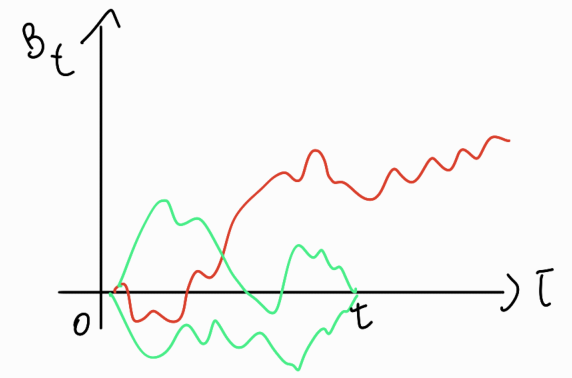
\includegraphics[width=0.5\linewidth]{img/screenshot036}
	\caption{This time I remembered to turn off the lines.}
	\label{fig:screenshot036}
\end{figure}
\begin{theorem}
	The \emph{Brownian bridge $\widetilde{B}_{t}$} is a Gaussian process with covariance function
	\begin{align*}
		\ev{\widetilde{B}_{s}\widetilde{B}_{\omega}}&=\ev{B_{s}B_{\omega}|B_{0}=B_{t}=0}\\
		&=\frac{1}{t}\left[(s\wedge\omega)((t-s)\wedge(t-\omega))\right]\qquad0<s,\omega\leq t
	\end{align*}
	and mean
	\begin{equation*}
		\ev{\widetilde{B}_{s}}=0.
	\end{equation*}
\end{theorem}
So the Gaussian bridge is basically a \bwm{} to which we impose the condition that it must start at 0 at time 0 and end at 0 at time $t$. Is a ``selection'' of the infinitely possible sample paths (among which there are some that start at 0 and end at 0 at $t$) and as we know, ``selecting'' means conditioning.
\begin{fancyproof}
	Consider $(B_{s}B_{\omega}|B_{t})$ for $\omega<s<t$. The vector $(B_{t},B_{s},B_{\omega})$ has covariance matrix
	\begin{equation*}
		\Sigma=\left[\begin{array}{c;{6pt/2pt}cc}
			t&s&\omega\\ \hdashline[6pt/2pt]
			s&s&\omega\\
			\omega&\omega&\omega
		\end{array}\right].\tag*{\faBaseballBall}\label{baseball}
	\end{equation*}
	Note that \ref{baseball} is divided in a $1\times 1$ matrix $\Sigma_{11}$, a $1\times 2$ matrix $\Sigma_{12}$, a $2\times 1$ matrix $\Sigma_{21}$ and $2\times2$ matrix $\Sigma_{22}$. The covariance matrix $\Sigma_{2|1}$ (that is the conditional covariance of one subset of random variables ``2'', in this case the Gaussian sub-vector $(B_{s},B_{\omega})$ to another subset of random variables ``1'', in this case the sub-vector $(B_{t})$) of $(B_{s},B_{\omega})$ conditioned on $B_{t}$ is therefore 
	\begin{align*}
		\Sigma_{2|1}&=\Sigma_{22}-\Sigma_{21}\Sigma_{11}^{-1}\Sigma_{12}\\
		&=\begin{bmatrix}
			s&\omega\\
			\omega&\omega
		\end{bmatrix}-\frac{1}{t}\begin{bmatrix}
		s\\ \omega
		\end{bmatrix}\begin{bmatrix}
		s&\omega
		\end{bmatrix}\\
		&=\begin{bmatrix}
			s&\omega\\
			\omega&\omega
		\end{bmatrix}-\frac{1}{t}\begin{bmatrix}
		s^{2}&s\omega\\
		s\omega&\omega^{2}
		\end{bmatrix}\\
		&=\begin{bmatrix}
			s-\frac{1}{t}s^{2}&\omega-\frac{1}{t}s\omega\\
			\omega-\frac{1}{t}s\omega&\omega-\frac{1}{t}\omega^{2}
		\end{bmatrix}.
	\end{align*}
	This means that 
	\begin{align*}
		\ev{B_{s}B_{\omega}|B_{0}=B_{t}=0}&=\begin{cases}
			\omega-\frac{1}{t}s\omega&\omega<s\\
			s-\frac{1}{t}s\omega&\omega>s
		\end{cases}\\
		&=\frac{1}{t}(s\wedge\omega)\left[(t-s)\wedge(t-\omega)\right].
	\end{align*}
	So the variance of $\widetilde{B}$ is
	\begin{equation*}
		\var\widetilde{B}_{s}=\frac{1}{t}s(t-s).
	\end{equation*}
\end{fancyproof} 
Question: are the increments of $\widetilde{B}$ independent? Actually not... Because we have the conditions that the process must be at 0 at time $t$. So the increments, having to reach a certain point, are dependent on their position respect to $t$! Also, it doesn't have to be 0: I can also set a value $A$ at time $\vartheta$ and a value $B$ at time $t$ and only consider the sample paths that go through these points.
\begin{figure}[h]
	\centering
	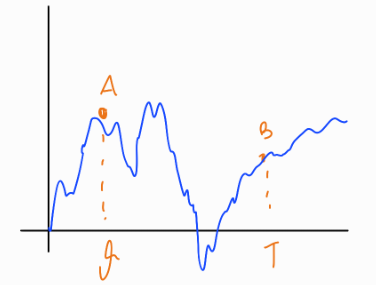
\includegraphics[width=0.4\linewidth]{img/screenshot037}
	\caption{This is... cool I guess?}
	\label{fig:screenshot037}
\end{figure}
\begin{remark}
	The Brownian bridge can be represented as 
	\begin{equation*}
		X_{s}=B_{s}-\frac{s}{t}B_{t}\qquad0\leq s\leq t.
	\end{equation*}
	If $t=1$ then
	\begin{equation*}
		X_{s}=B_{s}-sB_{t}.
	\end{equation*}
	At time 1 this is equal to 0 and it has the same distribution as the equation above. Another representation is
	\begin{equation*}
		Y_{s}=(1-s)\frac{B_{s}}{1-t}\qquad0\leq s\leq t.
	\end{equation*}
\end{remark}
	These representations are equal to the Brownian bridge in distribution. The shape of the sample path, of course, can be different.\par
	Why do we care? There are many reasons:
	\begin{enumerate}
		\item Simulations: imagine that we want to simulate a \bwm. We know that we can obtain a simulated \bwm by partitioning our times and then extracting a Gaussian \rv{} to get the increment between times.
		\begin{figure}[h]
			\centering
			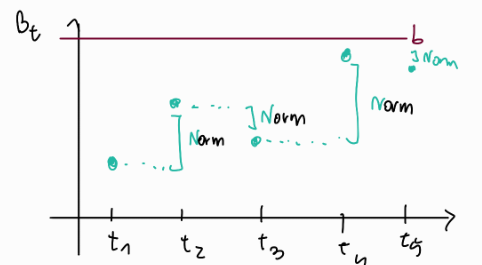
\includegraphics[width=0.5\linewidth]{img/screenshot038}
			\caption{Many little normal increments form a big Brownian noise.}
			\label{fig:screenshot038}
		\end{figure}
		Imagine we want to check whether the process crosses a threshold $b$. What if it does, but it happens in between two of the discrete values we computed? For example, in figure \ref{fig:screenshot038}, what if it crosses $b$ between the last two point? I could either recalculate everything with a finer mesh (huge waste of time) or... just study the Brownian bridge between those two points!
		\begin{figure}[h]
			\centering
			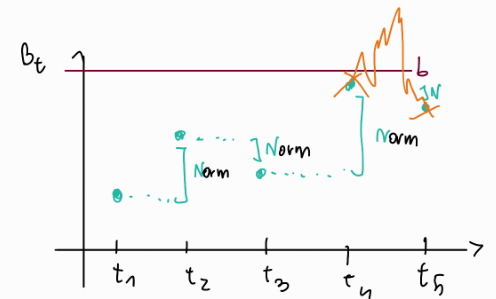
\includegraphics[width=0.5\linewidth]{img/screenshot039}
			\caption{I am going to do this motherfucker on Max/Msp.}
			\label{fig:screenshot039}
		\end{figure}
		\item The list could go on.
	\end{enumerate}
	\begin{remark}
		The Brownian bridge transition probability density function verifies the heat equation. It is the same as \bwm{} but with different boundary conditions. I don't really care.
	\end{remark}
\section{Properties of Brownian Paths}
\begin{figure}[H]
	\centering
	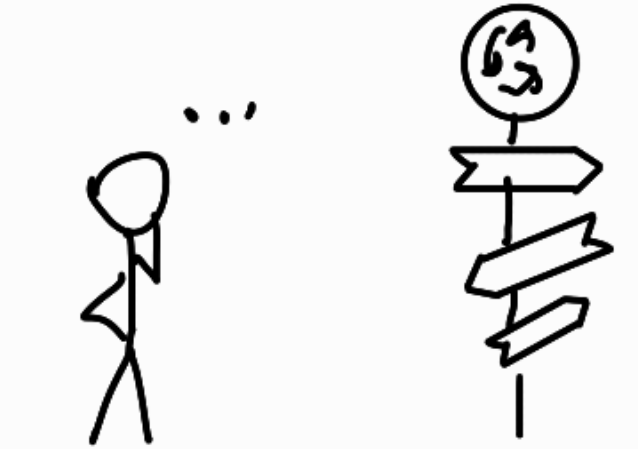
\includegraphics[width=0.3\linewidth]{img/screenshot040}
	\caption{Many paths but nowhere to go!}
	\label{fig:screenshot040}
\end{figure}
\subsection{Variation}
Subdivide an interval $[a,b]$ through a finite collection of disjoint intervals of the form $(s,t)$ whose union is $[a,b]$. Then we take 
\begin{equation*}
	\mathcal{A}=\text{subdivision with mesh }\norm{\mathcal{A}}=\sup\left\{t-s:(s,t]\in\mathcal{A}\right\}.
\end{equation*}
\begin{figure}[h]
	\centering
	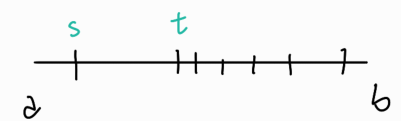
\includegraphics[width=0.5\linewidth]{img/screenshot041}
	\caption{In practice, we take the biggest subdivision. This helps when extending results to arbitrary subdivisions.}
	\label{fig:screenshot041}
\end{figure}
\begin{definition}
	Consider a right-continuous function $f:\R\to\R_{+}$. Fix an interval $[a,b]\in\R_{+}$. In general, for $p>0$, consider the sum
	\begin{equation*}
		\sum_{(s,t]\in\mathcal{A}}|f(t)-f(s)|^{p}.
	\end{equation*}
	The supremum of this sum over $[a,b]$
	\begin{equation*}
		\sup_{[a,b]}\sum_{(s,t]\in\mathcal{A}}|f(t)-f(s)|^{p}
	\end{equation*}
	is called \emph{p-variation}.\par
	Setting $p=2$ gives us the \emph{quadratic variation}. Setting $p=1$ gives us the \emph{total variation}.
\end{definition}
\begin{theorem}
	Let $(a,b]$ be fixed and let $\mathcal{A}_{n}$ be a sequence of subdivisions of it with the mesh going to 0:
	\begin{equation*}
		\norm{\mathcal{A}_{n}}\xrightarrow{n\to\infty}0.
	\end{equation*}
	The the sequence of \rv s
	\begin{equation*}
		V_{b}=\sum_{(s,t]\in\mathcal{A}_{n}}|B_{t}-B_{s}|^{2}
	\end{equation*}
	converges in $L^{2}$ and in probability to the length $b-a$.
\end{theorem}
\begin{figure}[H]
	\centering
	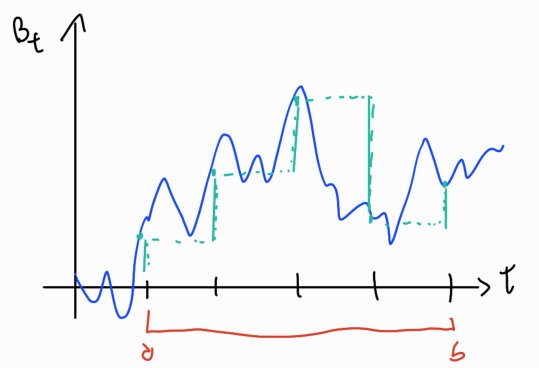
\includegraphics[width=0.5\linewidth]{img/screenshot042}
	\caption{Imagine that the gid becomes smaller and smaller.}
	\label{fig:screenshot042}
\end{figure}
\begin{fancyproof}
	We know that 
	\begin{equation*}
		|B_{t}-B_{s}|^{2}\sim(t-s)Z^{2}\qquad Z\distnorm{0,1}.
	\end{equation*}
	The intervals of the mesh are disjoint and their corresponding increments are therefore independent. Consider
	\begin{align*}
		\ev{V_{n}}&=\sum_{(s,t]\in\mathcal{A}_{n}}(t-s]\\ &=b-a
	\end{align*}
	and
	\begin{align*}
		\var V_{n}=\sum_{(s,t]\in\mathcal{A}_{n}}(t-s]^{2}\leq (b-a)\norm{\mathcal{A}_{n}}.
	\end{align*}
	This means that 
	\begin{equation*}
		\ev{(V_{n}-(b-a))^{2}}=\var V_{n}\xrightarrow{\text{since }\norm{\mathcal{A}_{n}}\to0}0.
	\end{equation*}
	So the sequence converges in $L^{2}$ and this implies convergence in probability. The limit
	\begin{equation*}
		\lim_{n\to\infty} V_{n} 
	\end{equation*} is the quadratic variation of $B$ over $(a,b]$.
\end{fancyproof}
\begin{theorem}
	For each $n\in\N$ let $\mathcal{A}_{n}$ be a subdivision of $(a,b]$ that consists of $2^{n}$ intervals of the same length. Then $V_{n}$ converges to $(b-a)$ almost surely.
\end{theorem}
\begin{fancyproof}
	For each $(s,t]$ we have length $(b-a)2^{-n}$ and this means that
	\begin{align*}
		\ev{V_{n}}&=b-a\\
		\var V_{n}&=2^{n}(b-a)^{2}2^{-n}.
	\end{align*}
	If we use Chebyshev's inequality we get
	\begin{equation*}
		\pr(|V_{n}-(b-a)|>\varepsilon)\leq\ubracketthin{\frac{1}{\varepsilon^{2}}(b-a)^{2}2^{-n}}_{\claptext{this is summable and finite}}
	\end{equation*}
	so using the Borel-Cantelli lemma 1 we get
	\begin{equation*}
		V_{n}\to(b-a)\;\as{}
	\end{equation*}
\end{fancyproof}
What about the total variation, tough?
\begin{proposition}
	For almost every $\omega$ the path $B(\omega)$ has infinite total variation over every interval $(a,b]$, $a<b$.
\end{proposition}
\begin{revise}
	A function $f:\R_{+}\to\R$ is said to be of \emph{bounded variation} on $[0,t]$ if $$V(f:[0,t])=\sup\left\{\sum|f(t_{i}-f(t_{i-1}))|\right\}$$ is finite for $0\leq t_{0}<t_{1}<\ldots<t_{n}<t$, $n\geq 1$.
\end{revise}
Here is an example of infinite variation function: 
\begin{equation*}
	f(t)=\begin{cases}
		t\sin\frac{1}{t}&t>0\\
		0&t=0.
	\end{cases}
\end{equation*}
\begin{figure}[h]
	\centering
	\definecolor{ccqqqq}{rgb}{0.8,0,0}
\begin{tikzpicture}[line cap=round,line join=round,>=triangle 45,x=1cm,y=1cm,scale=0.8]
	\begin{axis}[
		x=20cm,y=10cm,
		axis lines=middle,
		xmin=-0.1,
		xmax=0.2743397372103003,
		ymin=-0.25,
		ymax=0.18994586354928467,
		xtick={-0.2,-0.15000000000000002,...,0.25000000000000006},
		ytick={-0.45,-0.4,...,0.15000000000000002},]
		\clip(-0.23225009056530152,-0.48943429308000913) rectangle (0.2743397372103003,0.18994586354928467);
		\draw[line width=2pt,color=ccqqqq] (0,0) -- (0,0);
		\draw[line width=2pt,color=ccqqqq] (0,0) -- (0,0);
		\draw[line width=2pt,color=ccqqqq] (0.0013717670396117,0) -- (0.002057616210894837,0.0016707954043276663);
		\draw[line width=2pt,color=ccqqqq] (0.002057616210894837,0.0016707954043276663) -- (0.002743465382177974,0);
		\draw[line width=2pt,color=ccqqqq] (0.002743465382177974,0) -- (0.0034293145534611113,0.0018351059556873332);
		\draw[line width=2pt,color=ccqqqq] (0.0034293145534611113,0.0018351059556873332) -- (0.004115163724744249,-0.003669446248477033);
		\draw[line width=2pt,color=ccqqqq] (0.004115163724744249,-0.003669446248477033) -- (0.004801012896027386,0.003889138159670754);
		\draw[line width=2pt,color=ccqqqq] (0.004801012896027386,0.003889138159670754) -- (0.005486862067310524,0);
		\draw[line width=2pt,color=ccqqqq] (0.005486862067310524,0) -- (0.006172711238593661,-0.006035366697508066);
		\draw[line width=2pt,color=ccqqqq] (0.006172711238593661,-0.006035366697508066) -- (0.006858560409876799,0.006589812067339828);
		\draw[line width=2pt,color=ccqqqq] (0.006858560409876799,0.006589812067339828) -- (0.007544409581159936,0.004269761545325163);
		\draw[line width=2pt,color=ccqqqq] (0.007544409581159936,0.004269761545325163) -- (0.008230258752443074,0.007009839934872018);
		\draw[line width=2pt,color=ccqqqq] (0.008230258752443074,0.007009839934872018) -- (0.008916107923726211,-0.007204347281619517);
		\draw[line width=2pt,color=ccqqqq] (0.008916107923726211,-0.007204347281619517) -- (0.009601957095009349,-0.00437321108752983);
		\draw[line width=2pt,color=ccqqqq] (0.009601957095009349,-0.00437321108752983) -- (0.010287806266292486,0.0019118158517542653);
		\draw[line width=2pt,color=ccqqqq] (0.010287806266292486,0.0019118158517542653) -- (0.010973655437575624,0);
		\draw[line width=2pt,color=ccqqqq] (0.010973655437575624,0) -- (0.011659504608858761,-0.009442718024038727);
		\draw[line width=2pt,color=ccqqqq] (0.011659504608858761,-0.009442718024038727) -- (0.012345353780141899,-0.007755711575304749);
		\draw[line width=2pt,color=ccqqqq] (0.012345353780141899,-0.007755711575304749) -- (0.013031202951425036,0.01268764667511411);
		\draw[line width=2pt,color=ccqqqq] (0.013031202951425036,0.01268764667511411) -- (0.013717052122708174,-0.008250287629027167);
		\draw[line width=2pt,color=ccqqqq] (0.013717052122708174,-0.008250287629027167) -- (0.014402901293991311,0.0044679703222995715);
		\draw[line width=2pt,color=ccqqqq] (0.014402901293991311,0.0044679703222995715) -- (0.015088750465274449,-0.004474805340643384);
		\draw[line width=2pt,color=ccqqqq] (0.015088750465274449,-0.004474805340643384) -- (0.015774599636557585,0.00839525465338158);
		\draw[line width=2pt,color=ccqqqq] (0.015774599636557585,0.00839525465338158) -- (0.01646044880784072,-0.014370811416521842);
		\draw[line width=2pt,color=ccqqqq] (0.01646044880784072,-0.014370811416521842) -- (0.017146297979123856,0.016797105485642037);
		\draw[line width=2pt,color=ccqqqq] (0.017146297979123856,0.016797105485642037) -- (0.017832147150406992,-0.008078659020638453);
		\draw[line width=2pt,color=ccqqqq] (0.017832147150406992,-0.008078659020638453) -- (0.018517996321690128,-0.010371026945081753);
		\draw[line width=2pt,color=ccqqqq] (0.018517996321690128,-0.010371026945081753) -- (0.019203845492973264,0.018668724021365053);
		\draw[line width=2pt,color=ccqqqq] (0.019203845492973264,0.018668724021365053) -- (0.0198896946642564,0);
		\draw[line width=2pt,color=ccqqqq] (0.0198896946642564,0) -- (0.020575543835539535,-0.02048605944062804);
		\draw[line width=2pt,color=ccqqqq] (0.020575543835539535,-0.02048605944062804) -- (0.02126139300682267,0.0019169344926051953);
		\draw[line width=2pt,color=ccqqqq] (0.02126139300682267,0.0019169344926051953) -- (0.021947242178105807,0.021945981643765104);
		\draw[line width=2pt,color=ccqqqq] (0.021947242178105807,0.021945981643765104) -- (0.022633091349388942,0.0045141728046842085);
		\draw[line width=2pt,color=ccqqqq] (0.022633091349388942,0.0045141728046842085) -- (0.023318940520672078,-0.020768266579005955);
		\draw[line width=2pt,color=ccqqqq] (0.023318940520672078,-0.020768266579005955) -- (0.024004789691955214,-0.01751244209074995);
		\draw[line width=2pt,color=ccqqqq] (0.024004789691955214,-0.01751244209074995) -- (0.02469063886323835,0.008222948439929637);
		\draw[line width=2pt,color=ccqqqq] (0.02469063886323835,0.008222948439929637) -- (0.025376488034521485,0.025139933156518857);
		\draw[line width=2pt,color=ccqqqq] (0.025376488034521485,0.025139933156518857) -- (0.02606233720580462,0.016193177456520526);
		\draw[line width=2pt,color=ccqqqq] (0.02606233720580462,0.016193177456520526) -- (0.026748186377087757,-0.008246315591643896);
		\draw[line width=2pt,color=ccqqqq] (0.026748186377087757,-0.008246315591643896) -- (0.027434035548370893,-0.02601747290702321);
		\draw[line width=2pt,color=ccqqqq] (0.027434035548370893,-0.02601747290702321) -- (0.02811988471965403,-0.02373026122996999);
		\draw[line width=2pt,color=ccqqqq] (0.02811988471965403,-0.02373026122996999) -- (0.028805733890937164,-0.004526460185331006);
		\draw[line width=2pt,color=ccqqqq] (0.028805733890937164,-0.004526460185331006) -- (0.0294915830622203,0.01783709133665563);
		\draw[line width=2pt,color=ccqqqq] (0.0294915830622203,0.01783709133665563) -- (0.030177432233503436,0.029835758266739745);
		\draw[line width=2pt,color=ccqqqq] (0.030177432233503436,0.029835758266739745) -- (0.03086328140478657,0.025718111709253866);
		\draw[line width=2pt,color=ccqqqq] (0.03086328140478657,0.025718111709253866) -- (0.03154913057606971,0.008739032728398273);
		\draw[line width=2pt,color=ccqqqq] (0.03154913057606971,0.008739032728398273) -- (0.03223497974735284,-0.012366374614935206);
		\draw[line width=2pt,color=ccqqqq] (0.03223497974735284,-0.012366374614935206) -- (0.03292082891863598,-0.028391406618728608);
		\draw[line width=2pt,color=ccqqqq] (0.03292082891863598,-0.028391406618728608) -- (0.033606678089919115,-0.03347324956626086);
		\draw[line width=2pt,color=ccqqqq] (0.033606678089919115,-0.03347324956626086) -- (0.03429252726120225,-0.026572874090345717);
		\draw[line width=2pt,color=ccqqqq] (0.03429252726120225,-0.026572874090345717) -- (0.034978376432485386,-0.010828811716817384);
		\draw[line width=2pt,color=ccqqqq] (0.034978376432485386,-0.010828811716817384) -- (0.03566422560376852,0.008305263078285002);
		\draw[line width=2pt,color=ccqqqq] (0.03566422560376852,0.008305263078285002) -- (0.03635007477505166,0.02514948178640661);
		\draw[line width=2pt,color=ccqqqq] (0.03635007477505166,0.02514948178640661) -- (0.037035923946334794,0.0354114747089211);
		\draw[line width=2pt,color=ccqqqq] (0.037035923946334794,0.0354114747089211) -- (0.03772177311761793,0.03701669830356088);
		\draw[line width=2pt,color=ccqqqq] (0.03772177311761793,0.03701669830356088) -- (0.038407622288901065,0.0301752146331825);
		\draw[line width=2pt,color=ccqqqq] (0.038407622288901065,0.0301752146331825) -- (0.0390934714601842,0.01689783465934101);
		\draw[line width=2pt,color=ccqqqq] (0.0390934714601842,0.01689783465934101) -- (0.03977932063146734,0);
		\draw[line width=2pt,color=ccqqqq] (0.03977932063146734,0) -- (0.04046516980275047,-0.016504907912494475);
		\draw[line width=2pt,color=ccqqqq] (0.04046516980275047,-0.016504907912494475) -- (0.04115101897403361,-0.030422288097405527);
		\draw[line width=2pt,color=ccqqqq] (0.04115101897403361,-0.030422288097405527) -- (0.041836868145316744,-0.03943606892955303);
		\draw[line width=2pt,color=ccqqqq] (0.041836868145316744,-0.03943606892955303) -- (0.04252271731659988,-0.04247947215996387);
		\draw[line width=2pt,color=ccqqqq] (0.04252271731659988,-0.04247947215996387) -- (0.043208566487883016,-0.039481647986059576);
		\draw[line width=2pt,color=ccqqqq] (0.043208566487883016,-0.039481647986059576) -- (0.04389441565916615,-0.031205022478970956);
		\draw[line width=2pt,color=ccqqqq] (0.04389441565916615,-0.031205022478970956) -- (0.04458026483044929,-0.019000667690569673);
		\draw[line width=2pt,color=ccqqqq] (0.04458026483044929,-0.019000667690569673) -- (0.04526611400173242,-0.004538522896645146);
		\draw[line width=2pt,color=ccqqqq] (0.04526611400173242,-0.004538522896645146) -- (0.04595196317301556,0.010444365971511214);
		\draw[line width=2pt,color=ccqqqq] (0.04595196317301556,0.010444365971511214) -- (0.046637812344298694,0.024349927275829474);
		\draw[line width=2pt,color=ccqqqq] (0.046637812344298694,0.024349927275829474) -- (0.04732366151558183,0.03586605263205824);
		\draw[line width=2pt,color=ccqqqq] (0.04732366151558183,0.03586605263205824) -- (0.048009510686864966,0.04405242406419249);
		\draw[line width=2pt,color=ccqqqq] (0.048009510686864966,0.04405242406419249) -- (0.0486953598581481,0.04837099906102853);
		\draw[line width=2pt,color=ccqqqq] (0.0486953598581481,0.04837099906102853) -- (0.04938120902943124,0.04867158580258973);
		\draw[line width=2pt,color=ccqqqq] (0.04938120902943124,0.04867158580258973) -- (0.05006705820071437,0.04514484511562016);
		\draw[line width=2pt,color=ccqqqq] (0.05006705820071437,0.04514484511562016) -- (0.05075290737199751,0.038254966992250276);
		\draw[line width=2pt,color=ccqqqq] (0.05075290737199751,0.038254966992250276) -- (0.051438756543280645,0.02866288899978418);
		\draw[line width=2pt,color=ccqqqq] (0.051438756543280645,0.02866288899978418) -- (0.05212460571456378,0.017148849936582507);
		\draw[line width=2pt,color=ccqqqq] (0.05212460571456378,0.017148849936582507) -- (0.052810454885846916,0.004540763748761068);
		\draw[line width=2pt,color=ccqqqq] (0.052810454885846916,0.004540763748761068) -- (0.05349630405713005,-0.008347326146235639);
		\draw[line width=2pt,color=ccqqqq] (0.05349630405713005,-0.008347326146235639) -- (0.05418215322841319,-0.02076439957206718);
		\draw[line width=2pt,color=ccqqqq] (0.05418215322841319,-0.02076439957206718) -- (0.054868002399696324,-0.03205848165821328);
		\draw[line width=2pt,color=ccqqqq] (0.054868002399696324,-0.03205848165821328) -- (0.05555385157097946,-0.041699974630482924);
		\draw[line width=2pt,color=ccqqqq] (0.05555385157097946,-0.041699974630482924) -- (0.056239700742262595,-0.04929354378509632);
		\draw[line width=2pt,color=ccqqqq] (0.056239700742262595,-0.04929354378509632) -- (0.05692554991354573,-0.054580282113837905);
		\draw[line width=2pt,color=ccqqqq] (0.05692554991354573,-0.054580282113837905) -- (0.05761139908482887,-0.057432096000339716);
		\draw[line width=2pt,color=ccqqqq] (0.05761139908482887,-0.057432096000339716) -- (0.058297248256112,-0.057840274092610014);
		\draw[line width=2pt,color=ccqqqq] (0.058297248256112,-0.057840274092610014) -- (0.05898309742739514,-0.055900081923760093);
		\draw[line width=2pt,color=ccqqqq] (0.05898309742739514,-0.055900081923760093) -- (0.059668946598678274,-0.05179301685943027);
		\draw[line width=2pt,color=ccqqqq] (0.059668946598678274,-0.05179301685943027) -- (0.06035479576996141,-0.045768102541700634);
		\draw[line width=2pt,color=ccqqqq] (0.06035479576996141,-0.045768102541700634) -- (0.061040644941244546,-0.03812333050508974);
		\draw[line width=2pt,color=ccqqqq] (0.061040644941244546,-0.03812333050508974) -- (0.06172649411252768,-0.029188091529986148);
		\draw[line width=2pt,color=ccqqqq] (0.06172649411252768,-0.029188091529986148) -- (0.06241234328381082,-0.01930719547761205);
		\draw[line width=2pt,color=ccqqqq] (0.06241234328381082,-0.01930719547761205) -- (0.06309819245509396,-0.008826864607965378);
		\draw[line width=2pt,color=ccqqqq] (0.06309819245509396,-0.008826864607965378) -- (0.0637840416263771,0.0019170941920446639);
		\draw[line width=2pt,color=ccqqqq] (0.0637840416263771,0.0019170941920446639) -- (0.06446989079766025,0.012608877584015597);
		\draw[line width=2pt,color=ccqqqq] (0.06446989079766025,0.012608877584015597) -- (0.06515573996894339,0.02296008525671678);
		\draw[line width=2pt,color=ccqqqq] (0.06515573996894339,0.02296008525671678) -- (0.06584158914022653,0.03271506318587053);
		\draw[line width=2pt,color=ccqqqq] (0.06584158914022653,0.03271506318587053) -- (0.06652743831150967,0.04165437866424121);
		\draw[line width=2pt,color=ccqqqq] (0.06652743831150967,0.04165437866424121) -- (0.06721328748279282,0.049596648772135786);
		\draw[line width=2pt,color=ccqqqq] (0.06721328748279282,0.049596648772135786) -- (0.06789913665407596,0.05639895999221208);
		\draw[line width=2pt,color=ccqqqq] (0.06789913665407596,0.05639895999221208) -- (0.0685849858253591,0.06195611896131006);
		\draw[line width=2pt,color=ccqqqq] (0.0685849858253591,0.06195611896131006) -- (0.06927083499664224,0.06619896638251055);
		\draw[line width=2pt,color=ccqqqq] (0.06927083499664224,0.06619896638251055) -- (0.06995668416792539,0.06909197089922989);
		\draw[line width=2pt,color=ccqqqq] (0.06995668416792539,0.06909197089922989) -- (0.07064253333920853,0.07063029977112699);
		\draw[line width=2pt,color=ccqqqq] (0.07064253333920853,0.07063029977112699) -- (0.07132838251049167,0.07083654052337914);
		\draw[line width=2pt,color=ccqqqq] (0.07132838251049167,0.07083654052337914) -- (0.07201423168177482,0.06975722396344874);
		\draw[line width=2pt,color=ccqqqq] (0.07201423168177482,0.06975722396344874) -- (0.07270008085305796,0.06745927528301239);
		\draw[line width=2pt,color=ccqqqq] (0.07270008085305796,0.06745927528301239) -- (0.0733859300243411,0.06402649726601813);
		\draw[line width=2pt,color=ccqqqq] (0.0733859300243411,0.06402649726601813) -- (0.07407177919562424,0.05955616850943199);
		\draw[line width=2pt,color=ccqqqq] (0.07407177919562424,0.05955616850943199) -- (0.07475762836690739,0.054155820409577664);
		\draw[line width=2pt,color=ccqqqq] (0.07475762836690739,0.054155820409577664) -- (0.07544347753819053,0.047940239675547044);
		\draw[line width=2pt,color=ccqqqq] (0.07544347753819053,0.047940239675547044) -- (0.07612932670947367,0.04102872836780393);
		\draw[line width=2pt,color=ccqqqq] (0.07612932670947367,0.04102872836780393) -- (0.07681517588075681,0.03354264089020927);
		\draw[line width=2pt,color=ccqqqq] (0.07681517588075681,0.03354264089020927) -- (0.07750102505203996,0.02560320688151484);
		\draw[line width=2pt,color=ccqqqq] (0.07750102505203996,0.02560320688151484) -- (0.0781868742233231,0.01732964040475531);
		\draw[line width=2pt,color=ccqqqq] (0.0781868742233231,0.01732964040475531) -- (0.07887272339460624,0.008837529038291035);
		\draw[line width=2pt,color=ccqqqq] (0.07887272339460624,0.008837529038291035) -- (0.07955857256588938,0);
		\draw[line width=2pt,color=ccqqqq] (0.07955857256588938,0) -- (0.08024442173717253,-0.008365913562883185);
		\draw[line width=2pt,color=ccqqqq] (0.08024442173717253,-0.008365913562883185) -- (0.08093027090845567,-0.016875040277129646);
		\draw[line width=2pt,color=ccqqqq] (0.08093027090845567,-0.016875040277129646) -- (0.08161612007973881,-0.02519979897352254);
		\draw[line width=2pt,color=ccqqqq] (0.08161612007973881,-0.02519979897352254) -- (0.08230196925102196,-0.03325810194005816);
		\draw[line width=2pt,color=ccqqqq] (0.08230196925102196,-0.03325810194005816) -- (0.0829878184223051,-0.04097613819593458);
		\draw[line width=2pt,color=ccqqqq] (0.0829878184223051,-0.04097613819593458) -- (0.08367366759358824,-0.048288496295110034);
		\draw[line width=2pt,color=ccqqqq] (0.08367366759358824,-0.048288496295110034) -- (0.08435951676487138,-0.055138155616370976);
		\draw[line width=2pt,color=ccqqqq] (0.08435951676487138,-0.055138155616370976) -- (0.08504536593615453,-0.061476365356551495);
		\draw[line width=2pt,color=ccqqqq] (0.08504536593615453,-0.061476365356551495) -- (0.08573121510743767,-0.06726242925252732);
		\draw[line width=2pt,color=ccqqqq] (0.08573121510743767,-0.06726242925252732) -- (0.08641706427872081,-0.07246341272365821);
		\draw[line width=2pt,color=ccqqqq] (0.08641706427872081,-0.07246341272365821) -- (0.08710291345000395,-0.07705378770948848);
		\draw[line width=2pt,color=ccqqqq] (0.08710291345000395,-0.07705378770948848) -- (0.0877887626212871,-0.0810150290263213);
		\draw[line width=2pt,color=ccqqqq] (0.0877887626212871,-0.0810150290263213) -- (0.08847461179257024,-0.08433517461934986);
		\draw[line width=2pt,color=ccqqqq] (0.08847461179257024,-0.08433517461934986) -- (0.08916046096385338,-0.08700836067426841);
		\draw[line width=2pt,color=ccqqqq] (0.08916046096385338,-0.08700836067426841) -- (0.08984631013513653,-0.08903434119623387);
		\draw[line width=2pt,color=ccqqqq] (0.08984631013513653,-0.08903434119623387) -- (0.09053215930641967,-0.0904180003810015);
		\draw[line width=2pt,color=ccqqqq] (0.09053215930641967,-0.0904180003810015) -- (0.09121800847770281,-0.09116886490411905);
		\draw[line width=2pt,color=ccqqqq] (0.09121800847770281,-0.09116886490411905) -- (0.09190385764898595,-0.09130062214609494);
		\draw[line width=2pt,color=ccqqqq] (0.09190385764898595,-0.09130062214609494) -- (0.0925897068202691,-0.09083064935786472);
		\draw[line width=2pt,color=ccqqqq] (0.0925897068202691,-0.09083064935786472) -- (0.09327555599155224,-0.08977955785235206);
		\draw[line width=2pt,color=ccqqqq] (0.09327555599155224,-0.08977955785235206) -- (0.09396140516283538,-0.08817075548300876);
		\draw[line width=2pt,color=ccqqqq] (0.09396140516283538,-0.08817075548300876) -- (0.09464725433411852,-0.08603002993587257);
		\draw[line width=2pt,color=ccqqqq] (0.09464725433411852,-0.08603002993587257) -- (0.09533310350540167,-0.08338515471365944);
		\draw[line width=2pt,color=ccqqqq] (0.09533310350540167,-0.08338515471365944) -- (0.09601895267668481,-0.08026551912365737);
		\draw[line width=2pt,color=ccqqqq] (0.09601895267668481,-0.08026551912365737) -- (0.09670480184796795,-0.07670178309011783);
		\draw[line width=2pt,color=ccqqqq] (0.09670480184796795,-0.07670178309011783) -- (0.0973906510192511,-0.07272555719056793);
		\draw[line width=2pt,color=ccqqqq] (0.0973906510192511,-0.07272555719056793) -- (0.09807650019053424,-0.06836910795799646);
		\draw[line width=2pt,color=ccqqqq] (0.09807650019053424,-0.06836910795799646) -- (0.09876234936181738,-0.06366508819125652);
		\draw[line width=2pt,color=ccqqqq] (0.09876234936181738,-0.06366508819125652) -- (0.09944819853310052,-0.05864629176846328);
		\draw[line width=2pt,color=ccqqqq] (0.09944819853310052,-0.05864629176846328) -- (0.10013404770438367,-0.05334543225709716);
		\draw[line width=2pt,color=ccqqqq] (0.10013404770438367,-0.05334543225709716) -- (0.10081989687566681,-0.047794944454656214);
		\draw[line width=2pt,color=ccqqqq] (0.10081989687566681,-0.047794944454656214) -- (0.10150574604694995,-0.04202680787010927);
		\draw[line width=2pt,color=ccqqqq] (0.10150574604694995,-0.04202680787010927) -- (0.1021915952182331,-0.03607239106448607);
		\draw[line width=2pt,color=ccqqqq] (0.1021915952182331,-0.03607239106448607) -- (0.10287744438951624,-0.029962315704478656);
		\draw[line width=2pt,color=ccqqqq] (0.10287744438951624,-0.029962315704478656) -- (0.10356329356079938,-0.02372633914206033);
		\draw[line width=2pt,color=ccqqqq] (0.10356329356079938,-0.02372633914206033) -- (0.10424914273208252,-0.017393254312368638);
		\draw[line width=2pt,color=ccqqqq] (0.10424914273208252,-0.017393254312368638) -- (0.10493499190336567,-0.010990805738272507);
		\draw[line width=2pt,color=ccqqqq] (0.10493499190336567,-0.010990805738272507) -- (0.10562084107464881,-0.004545620440361467);
		\draw[line width=2pt,color=ccqqqq] (0.10562084107464881,-0.004545620440361467) -- (0.10630669024593195,0.0019168474269817166);
		\draw[line width=2pt,color=ccqqqq] (0.10630669024593195,0.0019168474269817166) -- (0.1069925394172151,0.008372359361418266);
		\draw[line width=2pt,color=ccqqqq] (0.1069925394172151,0.008372359361418266) -- (0.10767838858849824,0.014797923829605873);
		\draw[line width=2pt,color=ccqqqq] (0.10767838858849824,0.014797923829605873) -- (0.10836423775978138,0.021171817179911498);
		\draw[line width=2pt,color=ccqqqq] (0.10836423775978138,0.021171817179911498) -- (0.10905008693106452,0.027473595166682217);
		\draw[line width=2pt,color=ccqqqq] (0.10905008693106452,0.027473595166682217) -- (0.10973593610234766,0.03368409605001448);
		\draw[line width=2pt,color=ccqqqq] (0.10973593610234766,0.03368409605001448) -- (0.11042178527363081,0.039785436181148846);
		\draw[line width=2pt,color=ccqqqq] (0.11042178527363081,0.039785436181148846) -- (0.11110763444491395,0.04576099892880202);
		\draw[line width=2pt,color=ccqqqq] (0.11110763444491395,0.04576099892880202) -- (0.11179348361619709,0.05159541774667287);
		\draw[line width=2pt,color=ccqqqq] (0.11179348361619709,0.05159541774667287) -- (0.11247933278748024,0.057274554127670387);
		\draw[line width=2pt,color=ccqqqq] (0.11247933278748024,0.057274554127670387) -- (0.11316518195876338,0.06278547113665027);
		\draw[line width=2pt,color=ccqqqq] (0.11316518195876338,0.06278547113665027) -- (0.11385103113004652,0.06811640316100612);
		\draw[line width=2pt,color=ccqqqq] (0.11385103113004652,0.06811640316100612) -- (0.11453688030132966,0.07325672246770235);
		\draw[line width=2pt,color=ccqqqq] (0.11453688030132966,0.07325672246770235) -- (0.1152227294726128,0.07819690310650813);
		\draw[line width=2pt,color=ccqqqq] (0.1152227294726128,0.07819690310650813) -- (0.11590857864389595,0.08292848265248005);
		\draw[line width=2pt,color=ccqqqq] (0.11590857864389595,0.08292848265248005) -- (0.11659442781517909,0.08744402223629551);
		\draw[line width=2pt,color=ccqqqq] (0.11659442781517909,0.08744402223629551) -- (0.11728027698646223,0.09173706526894057);
		\draw[line width=2pt,color=ccqqqq] (0.11728027698646223,0.09173706526894057) -- (0.11796612615774538,0.09580209522754818);
		\draw[line width=2pt,color=ccqqqq] (0.11796612615774538,0.09580209522754818) -- (0.11865197532902852,0.0996344928318934);
		\draw[line width=2pt,color=ccqqqq] (0.11865197532902852,0.0996344928318934) -- (0.11933782450031166,0.1032304929061487);
		\draw[line width=2pt,color=ccqqqq] (0.11933782450031166,0.1032304929061487) -- (0.1200236736715948,0.10658714118796722);
		\draw[line width=2pt,color=ccqqqq] (0.1200236736715948,0.10658714118796722) -- (0.12070952284287795,0.1097022513167192);
		\draw[line width=2pt,color=ccqqqq] (0.12070952284287795,0.1097022513167192) -- (0.12139537201416109,0.11257436220470948);
		\draw[line width=2pt,color=ccqqqq] (0.12139537201416109,0.11257436220470948) -- (0.12208122118544423,0.11520269596934603);
		\draw[line width=2pt,color=ccqqqq] (0.12208122118544423,0.11520269596934603) -- (0.12276707035672738,0.11758711658044052);
		\draw[line width=2pt,color=ccqqqq] (0.12276707035672738,0.11758711658044052) -- (0.12345291952801052,0.11972808935499966);
		\draw[line width=2pt,color=ccqqqq] (0.12345291952801052,0.11972808935499966) -- (0.12413876869929366,0.1216266414119035);
		\draw[line width=2pt,color=ccqqqq] (0.12413876869929366,0.1216266414119035) -- (0.1248246178705768,0.12328432318067709);
		\draw[line width=2pt,color=ccqqqq] (0.1248246178705768,0.12328432318067709) -- (0.12551046704185995,0.12470317104202643);
		\draw[line width=2pt,color=ccqqqq] (0.12551046704185995,0.12470317104202643) -- (0.1261963162131431,0.12588567116284127);
		\draw[line width=2pt,color=ccqqqq] (0.1261963162131431,0.12588567116284127) -- (0.12688216538442623,0.12683472457485168);
		\draw[line width=2pt,color=ccqqqq] (0.12688216538442623,0.12683472457485168) -- (0.12756801455570937,0.12755361353397585);
		\draw[line width=2pt,color=ccqqqq] (0.12756801455570937,0.12755361353397585) -- (0.12825386372699252,0.12804596918650993);
		\draw[line width=2pt,color=ccqqqq] (0.12825386372699252,0.12804596918650993) -- (0.12893971289827566,0.12831574055859818);
		\draw[line width=2pt,color=ccqqqq] (0.12893971289827566,0.12831574055859818) -- (0.1296255620695588,0.12836716487679564);
		\draw[line width=2pt,color=ccqqqq] (0.1296255620695588,0.12836716487679564) -- (0.13031141124084195,0.12820473921990858);
		\draw[line width=2pt,color=ccqqqq] (0.13031141124084195,0.12820473921990858) -- (0.1309972604121251,0.12783319349559263);
		\draw[line width=2pt,color=ccqqqq] (0.1309972604121251,0.12783319349559263) -- (0.13168310958340823,0.12725746472932842);
		\draw[line width=2pt,color=ccqqqq] (0.13168310958340823,0.12725746472932842) -- (0.13236895875469137,0.1264826726483057);
		\draw[line width=2pt,color=ccqqqq] (0.13236895875469137,0.1264826726483057) -- (0.13305480792597452,0.12551409653836593);
		\draw[line width=2pt,color=ccqqqq] (0.13305480792597452,0.12551409653836593) -- (0.13374065709725766,0.12435715334841234);
		\draw[line width=2pt,color=ccqqqq] (0.13374065709725766,0.12435715334841234) -- (0.1344265062685408,0.12301737701354078);
		\draw[line width=2pt,color=ccqqqq] (0.1344265062685408,0.12301737701354078) -- (0.13511235543982394,0.12150039896551453);
		\draw[line width=2pt,color=ccqqqq] (0.13511235543982394,0.12150039896551453) -- (0.1357982046111071,0.1198119297970563);
		\draw[line width=2pt,color=ccqqqq] (0.1357982046111071,0.1198119297970563) -- (0.13648405378239023,0.11795774204470492);
		\draw[line width=2pt,color=ccqqqq] (0.13648405378239023,0.11795774204470492) -- (0.13716990295367337,0.11594365405364969);
		\draw[line width=2pt,color=ccqqqq] (0.13716990295367337,0.11594365405364969) -- (0.13785575212495652,0.11377551488695833);
		\draw[line width=2pt,color=ccqqqq] (0.13785575212495652,0.11377551488695833) -- (0.13854160129623966,0.11145919024093082);
		\draw[line width=2pt,color=ccqqqq] (0.13854160129623966,0.11145919024093082) -- (0.1392274504675228,0.10900054932789521);
		\draw[line width=2pt,color=ccqqqq] (0.1392274504675228,0.10900054932789521) -- (0.13991329963880594,0.10640545268758847);
		\draw[line width=2pt,color=ccqqqq] (0.13991329963880594,0.10640545268758847) -- (0.1405991488100891,0.1036797408883044);
		\draw[line width=2pt,color=ccqqqq] (0.1405991488100891,0.1036797408883044) -- (0.14128499798137223,0.10082922407921271);
		\draw[line width=2pt,color=ccqqqq] (0.14128499798137223,0.10082922407921271) -- (0.14197084715265537,0.09785967235564032);
		\draw[line width=2pt,color=ccqqqq] (0.14197084715265537,0.09785967235564032) -- (0.14265669632393851,0.0947768068996269);
		\draw[line width=2pt,color=ccqqqq] (0.14265669632393851,0.0947768068996269) -- (0.14334254549522166,0.09158629185871411);
		\draw[line width=2pt,color=ccqqqq] (0.14334254549522166,0.09158629185871411) -- (0.1440283946665048,0.08829372692666902);
		\draw[line width=2pt,color=ccqqqq] (0.1440283946665048,0.08829372692666902) -- (0.14471424383778794,0.08490464059067536);
		\draw[line width=2pt,color=ccqqqq] (0.14471424383778794,0.08490464059067536) -- (0.14540009300907109,0.08142448401042301);
		\draw[line width=2pt,color=ccqqqq] (0.14540009300907109,0.08142448401042301) -- (0.14608594218035423,0.07785862549548817);
		\draw[line width=2pt,color=ccqqqq] (0.14608594218035423,0.07785862549548817) -- (0.14677179135163737,0.07421234554839559);
		\draw[line width=2pt,color=ccqqqq] (0.14677179135163737,0.07421234554839559) -- (0.1474576405229205,0.07049083244179417);
		\draw[line width=2pt,color=ccqqqq] (0.1474576405229205,0.07049083244179417) -- (0.14814348969420366,0.06669917829924088);
		\draw[line width=2pt,color=ccqqqq] (0.14814348969420366,0.06669917829924088) -- (0.1488293388654868,0.06284237565016719);
		\draw[line width=2pt,color=ccqqqq] (0.1488293388654868,0.06284237565016719) -- (0.14951518803676994,0.05892531443069325);
		\draw[line width=2pt,color=ccqqqq] (0.14951518803676994,0.05892531443069325) -- (0.15020103720805308,0.0549527794030498);
		\draw[line width=2pt,color=ccqqqq] (0.15020103720805308,0.0549527794030498) -- (0.15088688637933623,0.05092944796745627);
		\draw[line width=2pt,color=ccqqqq] (0.15088688637933623,0.05092944796745627) -- (0.15157273555061937,0.046859888341389974);
		\draw[line width=2pt,color=ccqqqq] (0.15157273555061937,0.046859888341389974) -- (0.1522585847219025,0.04274855808225263);
		\draw[line width=2pt,color=ccqqqq] (0.1522585847219025,0.04274855808225263) -- (0.15294443389318566,0.0385998029304973);
		\draw[line width=2pt,color=ccqqqq] (0.15294443389318566,0.0385998029304973) -- (0.1536302830644688,0.03441785595131609);
		\draw[line width=2pt,color=ccqqqq] (0.1536302830644688,0.03441785595131609) -- (0.15431613223575194,0.030206836954009553);
		\draw[line width=2pt,color=ccqqqq] (0.15431613223575194,0.030206836954009553) -- (0.15500198140703508,0.02597075216914902);
		\draw[line width=2pt,color=ccqqqq] (0.15500198140703508,0.02597075216914902) -- (0.15568783057831823,0.02171349416461268);
		\draw[line width=2pt,color=ccqqqq] (0.15568783057831823,0.02171349416461268) -- (0.15637367974960137,0.017438841982520107);
		\draw[line width=2pt,color=ccqqqq] (0.15637367974960137,0.017438841982520107) -- (0.1570595289208845,0.013150461480002628);
		\draw[line width=2pt,color=ccqqqq] (0.1570595289208845,0.013150461480002628) -- (0.15774537809216765,0.008851905857631513);
		\draw[line width=2pt,color=ccqqqq] (0.15774537809216765,0.008851905857631513) -- (0.1584312272634508,0.0045466163601833335);
		\draw[line width=2pt,color=ccqqqq] (0.1584312272634508,0.0045466163601833335) -- (0.15911707643473394,0);
		\draw[line width=2pt,color=ccqqqq] (0.15911707643473394,0) -- (0.15980292560601708,-0.004070953764013781);
		\draw[line width=2pt,color=ccqqqq] (0.15980292560601708,-0.004070953764013781) -- (0.16048877477730022,-0.0083769032449131);
		\draw[line width=2pt,color=ccqqqq] (0.16048877477730022,-0.0083769032449131) -- (0.16117462394858337,-0.012676921922241347);
		\draw[line width=2pt,color=ccqqqq] (0.16117462394858337,-0.012676921922241347) -- (0.1618604731198665,-0.01696811275776177);
		\draw[line width=2pt,color=ccqqqq] (0.1618604731198665,-0.01696811275776177) -- (0.16254632229114965,-0.021247683602980252);
		\draw[line width=2pt,color=ccqqqq] (0.16254632229114965,-0.021247683602980252) -- (0.1632321714624328,-0.02551294565536029);
		\draw[line width=2pt,color=ccqqqq] (0.1632321714624328,-0.02551294565536029) -- (0.16391802063371594,-0.02976131183752768);
		\draw[line width=2pt,color=ccqqqq] (0.16391802063371594,-0.02976131183752768) -- (0.16460386980499908,-0.03399029510841187);
		\draw[line width=2pt,color=ccqqqq] (0.16460386980499908,-0.03399029510841187) -- (0.16528971897628222,-0.03819750671471119);
		\draw[line width=2pt,color=ccqqqq] (0.16528971897628222,-0.03819750671471119) -- (0.16597556814756537,-0.042380654390527066);
		\draw[line width=2pt,color=ccqqqq] (0.16597556814756537,-0.042380654390527066) -- (0.1666614173188485,-0.0465375405124998);
		\draw[line width=2pt,color=ccqqqq] (0.1666614173188485,-0.0465375405124998) -- (0.16734726649013165,-0.05066606021729267);
		\draw[line width=2pt,color=ccqqqq] (0.16734726649013165,-0.05066606021729267) -- (0.1680331156614148,-0.05476419948780353);
		\draw[line width=2pt,color=ccqqqq] (0.1680331156614148,-0.05476419948780353) -- (0.16871896483269794,-0.05883003321404455);
		\draw[line width=2pt,color=ccqqqq] (0.16871896483269794,-0.05883003321404455) -- (0.16940481400398108,-0.0628617232342142);
		\draw[line width=2pt,color=ccqqqq] (0.16940481400398108,-0.0628617232342142) -- (0.17009066317526422,-0.06685751636108483);
		\draw[line width=2pt,color=ccqqqq] (0.17009066317526422,-0.06685751636108483) -- (0.17077651234654737,-0.07081574239845874);
		\draw[line width=2pt,color=ccqqqq] (0.17077651234654737,-0.07081574239845874) -- (0.1714623615178305,-0.07473481215208859);
		\draw[line width=2pt,color=ccqqqq] (0.1714623615178305,-0.07473481215208859) -- (0.17214821068911365,-0.07861321543911964);
		\draw[line width=2pt,color=ccqqqq] (0.17214821068911365,-0.07861321543911964) -- (0.1728340598603968,-0.08244951909979961);
		\draw[line width=2pt,color=ccqqqq] (0.1728340598603968,-0.08244951909979961) -- (0.17351990903167994,-0.08624236501489681);
		\draw[line width=2pt,color=ccqqqq] (0.17351990903167994,-0.08624236501489681) -- (0.17420575820296308,-0.08999046813198917);
		\draw[line width=2pt,color=ccqqqq] (0.17420575820296308,-0.08999046813198917) -- (0.17489160737424622,-0.0936926145035164);
		\draw[line width=2pt,color=ccqqqq] (0.17489160737424622,-0.0936926145035164) -- (0.17557745654552936,-0.09734765933924287);
		\draw[line width=2pt,color=ccqqqq] (0.17557745654552936,-0.09734765933924287) -- (0.1762633057168125,-0.10095452507553489);
		\draw[line width=2pt,color=ccqqqq] (0.1762633057168125,-0.10095452507553489) -- (0.17694915488809565,-0.10451219946364351);
		\draw[line width=2pt,color=ccqqqq] (0.17694915488809565,-0.10451219946364351) -- (0.1776350040593788,-0.10801973367896783);
		\draw[line width=2pt,color=ccqqqq] (0.1776350040593788,-0.10801973367896783) -- (0.17832085323066194,-0.11147624045308435);
		\draw[line width=2pt,color=ccqqqq] (0.17832085323066194,-0.11147624045308435) -- (0.17900670240194508,-0.11488089223014068);
		\draw[line width=2pt,color=ccqqqq] (0.17900670240194508,-0.11488089223014068) -- (0.17969255157322822,-0.1182329193490439);
		\draw[line width=2pt,color=ccqqqq] (0.17969255157322822,-0.1182329193490439) -- (0.18037840074451136,-0.12153160825271071);
		\draw[line width=2pt,color=ccqqqq] (0.18037840074451136,-0.12153160825271071) -- (0.1810642499157945,-0.12477629972549835);
		\draw[line width=2pt,color=ccqqqq] (0.1810642499157945,-0.12477629972549835) -- (0.18175009908707765,-0.12796638715979358);
		\draw[line width=2pt,color=ccqqqq] (0.18175009908707765,-0.12796638715979358) -- (0.1824359482583608,-0.13110131485260887);
		\draw[line width=2pt,color=ccqqqq] (0.1824359482583608,-0.13110131485260887) -- (0.18312179742964393,-0.13418057633290895);
		\draw[line width=2pt,color=ccqqqq] (0.18312179742964393,-0.13418057633290895) -- (0.18380764660092708,-0.13720371272028384);
		\draw[line width=2pt,color=ccqqqq] (0.18380764660092708,-0.13720371272028384) -- (0.18449349577221022,-0.14017031111547226);
		\draw[line width=2pt,color=ccqqqq] (0.18449349577221022,-0.14017031111547226) -- (0.18517934494349336,-0.14308000302314663);
		\draw[line width=2pt,color=ccqqqq] (0.18517934494349336,-0.14308000302314663) -- (0.1858651941147765,-0.14593246280727748);
		\draw[line width=2pt,color=ccqqqq] (0.1858651941147765,-0.14593246280727748) -- (0.18655104328605965,-0.1487274061793128);
		\draw[line width=2pt,color=ccqqqq] (0.18655104328605965,-0.1487274061793128) -- (0.1872368924573428,-0.15146458871932872);
		\draw[line width=2pt,color=ccqqqq] (0.1872368924573428,-0.15146458871932872) -- (0.18792274162862593,-0.15414380443023726);
		\draw[line width=2pt,color=ccqqqq] (0.18792274162862593,-0.15414380443023726) -- (0.18860859079990908,-0.15676488432506994);
		\draw[line width=2pt,color=ccqqqq] (0.18860859079990908,-0.15676488432506994) -- (0.18929443997119222,-0.15932769504729702);
		\draw[line width=2pt,color=ccqqqq] (0.18929443997119222,-0.15932769504729702) -- (0.18998028914247536,-0.16183213752408454);
		\draw[line width=2pt,color=ccqqqq] (0.18998028914247536,-0.16183213752408454) -- (0.1906661383137585,-0.16427814565233995);
		\draw[line width=2pt,color=ccqqqq] (0.1906661383137585,-0.16427814565233995) -- (0.19135198748504165,-0.1666656850173541);
		\draw[line width=2pt,color=ccqqqq] (0.19135198748504165,-0.1666656850173541) -- (0.1920378366563248,-0.16899475164379932);
		\draw[line width=2pt,color=ccqqqq] (0.1920378366563248,-0.16899475164379932) -- (0.19272368582760793,-0.17126537077880868);
		\draw[line width=2pt,color=ccqqqq] (0.19272368582760793,-0.17126537077880868) -- (0.19340953499889108,-0.17347759570682617);
		\draw[line width=2pt,color=ccqqqq] (0.19340953499889108,-0.17347759570682617) -- (0.19409538417017422,-0.17563150659588278);
		\draw[line width=2pt,color=ccqqqq] (0.19409538417017422,-0.17563150659588278) -- (0.19478123334145736,-0.17772720937492953);
		\draw[line width=2pt,color=ccqqqq] (0.19478123334145736,-0.17772720937492953) -- (0.1954670825127405,-0.1797648346418285);
		\draw[line width=2pt,color=ccqqqq] (0.1954670825127405,-0.1797648346418285) -- (0.19615293168402365,-0.18174453660158454);
		\draw[line width=2pt,color=ccqqqq] (0.19615293168402365,-0.18174453660158454) -- (0.1968387808553068,-0.18366649203437566);
		\draw[line width=2pt,color=ccqqqq] (0.1968387808553068,-0.18366649203437566) -- (0.19752463002658993,-0.1855308992929269);
		\draw[line width=2pt,color=ccqqqq] (0.19752463002658993,-0.1855308992929269) -- (0.19821047919787307,-0.1873379773287538);
		\draw[line width=2pt,color=ccqqqq] (0.19821047919787307,-0.1873379773287538) -- (0.19889632836915622,-0.18908796474678918);
		\draw[line width=2pt,color=ccqqqq] (0.19889632836915622,-0.18908796474678918) -- (0.19958217754043936,-0.19078111888789648);
		\draw[line width=2pt,color=ccqqqq] (0.19958217754043936,-0.19078111888789648) -- (0.2002680267117225,-0.19241771493876217);
		\draw[line width=2pt,color=ccqqqq] (0.2002680267117225,-0.19241771493876217) -- (0.20095387588300564,-0.19399804506865193);
		\draw[line width=2pt,color=ccqqqq] (0.20095387588300564,-0.19399804506865193) -- (0.2016397250542888,-0.19552241759250996);
		\draw[line width=2pt,color=ccqqqq] (0.2016397250542888,-0.19552241759250996) -- (0.20232557422557193,-0.19699115615987453);
		\draw[line width=2pt,color=ccqqqq] (0.20232557422557193,-0.19699115615987453) -- (0.20301142339685507,-0.19840459896908058);
		\draw[line width=2pt,color=ccqqqq] (0.20301142339685507,-0.19840459896908058) -- (0.20369727256813822,-0.19976309800621672);
		\draw[line width=2pt,color=ccqqqq] (0.20369727256813822,-0.19976309800621672) -- (0.20438312173942136,-0.20106701830830362);
		\draw[line width=2pt,color=ccqqqq] (0.20438312173942136,-0.20106701830830362) -- (0.2050689709107045,-0.20231673725016033);
		\draw[line width=2pt,color=ccqqqq] (0.2050689709107045,-0.20231673725016033) -- (0.20575482008198764,-0.2035126438544258);
		\draw[line width=2pt,color=ccqqqq] (0.20575482008198764,-0.2035126438544258) -- (0.2064406692532708,-0.20465513812420427);
		\draw[line width=2pt,color=ccqqqq] (0.2064406692532708,-0.20465513812420427) -- (0.20712651842455393,-0.20574463039780713);
		\draw[line width=2pt,color=ccqqqq] (0.20712651842455393,-0.20574463039780713) -- (0.20781236759583707,-0.20678154072506447);
		\draw[line width=2pt,color=ccqqqq] (0.20781236759583707,-0.20678154072506447) -- (0.20849821676712021,-0.20776629826468593);
		\draw[line width=2pt,color=ccqqqq] (0.20849821676712021,-0.20776629826468593) -- (0.20918406593840336,-0.20869934070215404);
		\draw[line width=2pt,color=ccqqqq] (0.20918406593840336,-0.20869934070215404) -- (0.2098699151096865,-0.20958111368763735);
		\draw[line width=2pt,color=ccqqqq] (0.2098699151096865,-0.20958111368763735) -- (0.21055576428096964,-0.21041207029341777);
		\draw[line width=2pt,color=ccqqqq] (0.21055576428096964,-0.21041207029341777) -- (0.21124161345225279,-0.21119267049033152);
		\draw[line width=2pt,color=ccqqqq] (0.21124161345225279,-0.21119267049033152) -- (0.21192746262353593,-0.21192338064272945);
		\draw[line width=2pt,color=ccqqqq] (0.21192746262353593,-0.21192338064272945) -- (0.21261331179481907,-0.21260467302147001);
		\draw[line width=2pt,color=ccqqqq] (0.21261331179481907,-0.21260467302147001) -- (0.2132991609661022,-0.21323702533446406);
		\draw[line width=2pt,color=ccqqqq] (0.2132991609661022,-0.21323702533446406) -- (0.21398501013738536,-0.2138209202742989);
		\draw[line width=2pt,color=ccqqqq] (0.21398501013738536,-0.2138209202742989) -- (0.2146708593086685,-0.21435684508247593);
		\draw[line width=2pt,color=ccqqqq] (0.2146708593086685,-0.21435684508247593) -- (0.21535670847995164,-0.21484529112980458);
		\draw[line width=2pt,color=ccqqqq] (0.21535670847995164,-0.21484529112980458) -- (0.21604255765123478,-0.21528675351250265);
		\draw[line width=2pt,color=ccqqqq] (0.21604255765123478,-0.21528675351250265) -- (0.21672840682251793,-0.21568173066356094);
		\draw[line width=2pt,color=ccqqqq] (0.21672840682251793,-0.21568173066356094) -- (0.21741425599380107,-0.21603072397893963);
		\draw[line width=2pt,color=ccqqqq] (0.21741425599380107,-0.21603072397893963) -- (0.2181001051650842,-0.2163342374581703);
		\draw[line width=2pt,color=ccqqqq] (0.2181001051650842,-0.2163342374581703) -- (0.21878595433636736,-0.2165927773589473);
		\draw[line width=2pt,color=ccqqqq] (0.21878595433636736,-0.2165927773589473) -- (0.2194718035076505,-0.21680685186529994);
		\draw[line width=2pt,color=ccqqqq] (0.2194718035076505,-0.21680685186529994) -- (0.22015765267893364,-0.21697697076894507);
		\draw[line width=2pt,color=ccqqqq] (0.22015765267893364,-0.21697697076894507) -- (0.22084350185021678,-0.2171036451634293);
		\draw[line width=2pt,color=ccqqqq] (0.22084350185021678,-0.2171036451634293) -- (0.22152935102149993,-0.21718738715067684);
		\draw[line width=2pt,color=ccqqqq] (0.22152935102149993,-0.21718738715067684) -- (0.22221520019278307,-0.21722870955956913);
		\draw[line width=2pt,color=ccqqqq] (0.22221520019278307,-0.21722870955956913) -- (0.2229010493640662,-0.21722812567618946);
		\draw[line width=2pt,color=ccqqqq] (0.2229010493640662,-0.21722812567618946) -- (0.22358689853534935,-0.21718614898537483);
		\draw[line width=2pt,color=ccqqqq] (0.22358689853534935,-0.21718614898537483) -- (0.2242727477066325,-0.21710329292322544);
		\draw[line width=2pt,color=ccqqqq] (0.2242727477066325,-0.21710329292322544) -- (0.22495859687791564,-0.21698007064023084);
		\draw[line width=2pt,color=ccqqqq] (0.22495859687791564,-0.21698007064023084) -- (0.22564444604919878,-0.21681699477467878);
		\draw[line width=2pt,color=ccqqqq] (0.22564444604919878,-0.21681699477467878) -- (0.22633029522048193,-0.21661457723602248);
		\draw[line width=2pt,color=ccqqqq] (0.22633029522048193,-0.21661457723602248) -- (0.22701614439176507,-0.21637332899788897);
		\draw[line width=2pt,color=ccqqqq] (0.22701614439176507,-0.21637332899788897) -- (0.2277019935630482,-0.216093759900419);
		\draw[line width=2pt,color=ccqqqq] (0.2277019935630482,-0.216093759900419) -- (0.22838784273433135,-0.21577637846163805);
		\draw[line width=2pt,color=ccqqqq] (0.22838784273433135,-0.21577637846163805) -- (0.2290736919056145,-0.21542169169756376);
		\draw[line width=2pt,color=ccqqqq] (0.2290736919056145,-0.21542169169756376) -- (0.22975954107689764,-0.2150302049507642);
		\draw[line width=2pt,color=ccqqqq] (0.22975954107689764,-0.2150302049507642) -- (0.23044539024818078,-0.21460242172708918);
		\draw[line width=2pt,color=ccqqqq] (0.23044539024818078,-0.21460242172708918) -- (0.23113123941946392,-0.21413884354030133);
		\draw[line width=2pt,color=ccqqqq] (0.23113123941946392,-0.21413884354030133) -- (0.23181708859074707,-0.2136399697643457);
		\draw[line width=2pt,color=ccqqqq] (0.23181708859074707,-0.2136399697643457) -- (0.2325029377620302,-0.2131062974929982);
		\draw[line width=2pt,color=ccqqqq] (0.2325029377620302,-0.2131062974929982) -- (0.23318878693331335,-0.21253832140664564);
		\draw[line width=2pt,color=ccqqqq] (0.23318878693331335,-0.21253832140664564) -- (0.2338746361045965,-0.2119365336459518);
		\draw[line width=2pt,color=ccqqqq] (0.2338746361045965,-0.2119365336459518) -- (0.23456048527587964,-0.21130142369217558);
		\draw[line width=2pt,color=ccqqqq] (0.23456048527587964,-0.21130142369217558) -- (0.23524633444716278,-0.21063347825390927);
		\draw[line width=2pt,color=ccqqqq] (0.23524633444716278,-0.21063347825390927) -- (0.23593218361844592,-0.20993318116001564);
		\draw[line width=2pt,color=ccqqqq] (0.23593218361844592,-0.20993318116001564) -- (0.23661803278972907,-0.20920101325854576);
		\draw[line width=2pt,color=ccqqqq] (0.23661803278972907,-0.20920101325854576) -- (0.2373038819610122,-0.20843745232142688);
		\draw[line width=2pt,color=ccqqqq] (0.2373038819610122,-0.20843745232142688) -- (0.23798973113229535,-0.20764297295471626);
		\draw[line width=2pt,color=ccqqqq] (0.23798973113229535,-0.20764297295471626) -- (0.2386755803035785,-0.20681804651422125);
		\draw[line width=2pt,color=ccqqqq] (0.2386755803035785,-0.20681804651422125) -- (0.23936142947486164,-0.20596314102629404);
		\draw[line width=2pt,color=ccqqqq] (0.23936142947486164,-0.20596314102629404) -- (0.24004727864614478,-0.20507872111361236);
		\draw[line width=2pt,color=ccqqqq] (0.24004727864614478,-0.20507872111361236) -- (0.24073312781742792,-0.20416524792576538);
		\draw[line width=2pt,color=ccqqqq] (0.24073312781742792,-0.20416524792576538) -- (0.24141897698871106,-0.20322317907446782);
		\draw[line width=2pt,color=ccqqqq] (0.24141897698871106,-0.20322317907446782) -- (0.2421048261599942,-0.20225296857323205);
		\draw[line width=2pt,color=ccqqqq] (0.2421048261599942,-0.20225296857323205) -- (0.24279067533127735,-0.20125506678133104);
		\draw[line width=2pt,color=ccqqqq] (0.24279067533127735,-0.20125506678133104) -- (0.2434765245025605,-0.2002299203518926);
		\draw[line width=2pt,color=ccqqqq] (0.2434765245025605,-0.2002299203518926) -- (0.24416237367384364,-0.1991779721839682);
		\draw[line width=2pt,color=ccqqqq] (0.24416237367384364,-0.1991779721839682) -- (0.24484822284512678,-0.1980996613784248);
		\draw[line width=2pt,color=ccqqqq] (0.24484822284512678,-0.1980996613784248) -- (0.24553407201640992,-0.1969954231975151);
		\draw[line width=2pt,color=ccqqqq] (0.24553407201640992,-0.1969954231975151) -- (0.24621992118769306,-0.19586568902798077);
		\draw[line width=2pt,color=ccqqqq] (0.24621992118769306,-0.19586568902798077) -- (0.2469057703589762,-0.19471088634755548);
		\draw[line width=2pt,color=ccqqqq] (0.2469057703589762,-0.19471088634755548) -- (0.24759161953025935,-0.19353143869473027);
		\draw[line width=2pt,color=ccqqqq] (0.24759161953025935,-0.19353143869473027) -- (0.2482774687015425,-0.1923277656416555);
		\draw[line width=2pt,color=ccqqqq] (0.2482774687015425,-0.1923277656416555) -- (0.24896331787282563,-0.19110028277005298);
		\draw[line width=2pt,color=ccqqqq] (0.24896331787282563,-0.19110028277005298) -- (0.24964916704410878,-0.18984940165001643);
		\draw[line width=2pt,color=ccqqqq] (0.24964916704410878,-0.18984940165001643) -- (0.2503350162153919,-0.18857552982158587);
		\draw[line width=2pt,color=ccqqqq] (0.2503350162153919,-0.18857552982158587) -- (0.251020865386675,-0.18727907077897943);
		\draw[line width=2pt,color=ccqqqq] (0.251020865386675,-0.18727907077897943) -- (0.2517067145579581,-0.18596042395737586);
		\draw[line width=2pt,color=ccqqqq] (0.2517067145579581,-0.18596042395737586) -- (0.25239256372924124,-0.18461998472213956);
		\draw[line width=2pt,color=ccqqqq] (0.25239256372924124,-0.18461998472213956) -- (0.25307841290052435,-0.18325814436038618);
		\draw[line width=2pt,color=ccqqqq] (0.25307841290052435,-0.18325814436038618) -- (0.25376426207180747,-0.18187529007479042);
		\draw[line width=2pt,color=ccqqqq] (0.25376426207180747,-0.18187529007479042) -- (0.2544501112430906,-0.1804718049795385);
		\draw[line width=2pt,color=ccqqqq] (0.2544501112430906,-0.1804718049795385) -- (0.2551359604143737,-0.17904806809833373);
		\draw[line width=2pt,color=ccqqqq] (0.2551359604143737,-0.17904806809833373) -- (0.2558218095856568,-0.17760445436436484);
		\draw[line width=2pt,color=ccqqqq] (0.2558218095856568,-0.17760445436436484) -- (0.2565076587569399,-0.17614133462215092);
		\draw[line width=2pt,color=ccqqqq] (0.2565076587569399,-0.17614133462215092) -- (0.25719350792822304,-0.17465907563117894);
		\draw[line width=2pt,color=ccqqqq] (0.25719350792822304,-0.17465907563117894) -- (0.25787935709950616,-0.173158040071252);
		\draw[line width=2pt,color=ccqqqq] (0.25787935709950616,-0.173158040071252) -- (0.25856520627078927,-0.17163858654947242);
		\draw[line width=2pt,color=ccqqqq] (0.25856520627078927,-0.17163858654947242) -- (0.2592510554420724,-0.17010106960878166);
		\draw[line width=2pt,color=ccqqqq] (0.2592510554420724,-0.17010106960878166) -- (0.2599369046133555,-0.16854583973798565);
		\draw[line width=2pt,color=ccqqqq] (0.2599369046133555,-0.16854583973798565) -- (0.2606227537846386,-0.16697324338319472);
		\draw[line width=2pt,color=ccqqqq] (0.2606227537846386,-0.16697324338319472) -- (0.26130860295592173,-0.1653836229606096);
		\draw[line width=2pt,color=ccqqqq] (0.26130860295592173,-0.1653836229606096) -- (0.26199445212720485,-0.16377731687058958);
		\draw[line width=2pt,color=ccqqqq] (0.26199445212720485,-0.16377731687058958) -- (0.26268030129848796,-0.1621546595129371);
		\draw[line width=2pt,color=ccqqqq] (0.26268030129848796,-0.1621546595129371) -- (0.2633661504697711,-0.16051598130333958);
		\draw[line width=2pt,color=ccqqqq] (0.2633661504697711,-0.16051598130333958) -- (0.2640519996410542,-0.15886160869090923);
		\draw[line width=2pt,color=ccqqqq] (0.2640519996410542,-0.15886160869090923) -- (0.2647378488123373,-0.15719186417676279);
		\draw[line width=2pt,color=ccqqqq] (0.2647378488123373,-0.15719186417676279) -- (0.2654236979836204,-0.15550706633358868);
		\draw[line width=2pt,color=ccqqqq] (0.2654236979836204,-0.15550706633358868) -- (0.26610954715490354,-0.15380752982614565);
		\draw[line width=2pt,color=ccqqqq] (0.26610954715490354,-0.15380752982614565) -- (0.26679539632618665,-0.15209356543264557);
		\draw[line width=2pt,color=ccqqqq] (0.26679539632618665,-0.15209356543264557) -- (0.26748124549746977,-0.15036548006696793);
		\draw[line width=2pt,color=ccqqqq] (0.26748124549746977,-0.15036548006696793) -- (0.2681670946687529,-0.1486235768016616);
		\draw[line width=2pt,color=ccqqqq] (0.2681670946687529,-0.1486235768016616) -- (0.268852943840036,-0.14686815489168528);
		\draw[line width=2pt,color=ccqqqq] (0.268852943840036,-0.14686815489168528) -- (0.2695387930113191,-0.1450995097988465);
		\draw[line width=2pt,color=ccqqqq] (0.2695387930113191,-0.1450995097988465) -- (0.2702246421826022,-0.143317933216893);
		\draw[line width=2pt,color=ccqqqq] (0.2702246421826022,-0.143317933216893) -- (0.27091049135388534,-0.14152371309721895);
		\draw[line width=2pt,color=ccqqqq] (0.27091049135388534,-0.14152371309721895) -- (0.27159634052516846,-0.13971713367514477);
		\draw[line width=2pt,color=ccqqqq] (0.27159634052516846,-0.13971713367514477) -- (0.27228218969645157,-0.13789847549673417);
		\draw[line width=2pt,color=ccqqqq] (0.27228218969645157,-0.13789847549673417) -- (0.2729680388677347,-0.13606801544611133);
		\draw[line width=2pt,color=ccqqqq] (0.2729680388677347,-0.13606801544611133) -- (0.2736538880390178,-0.13422602677324405);
		\begin{scriptsize}
			\draw[color=ccqqqq] (0.0025876745585820702,0.009694134131454679) node {$f$};
		\end{scriptsize}
	\end{axis}
\end{tikzpicture}
	\caption{First time using the geogebra export function. I hate it.}
	\label{fig:codio}
\end{figure}
As we can see in figure \ref{fig:codio} the function has an extremely oscillatory nature. This is what happens with out \bwm, with the difference that the variations are very small. So much that taking their square makes them vanish.
\begin{fancyproof}
	Let $\Omega_{ab}$ be the set of $\omega$ such that $V_{n}\to(b-a)$. Pick $\omega\in\Omega_{ab}$ and let $v^{\star}$ be the total variation of $B(\omega)$. By contradiction, let $v^{\star}<\infty$. We have
	\begin{align*}
		\sum_{(s,t]\in\mathcal{A}_{n}}|B_{t}-B_{s}|^{2}&\leq\sup_{(s,t]\in\mathcal{A}_{n}}|B_{t}-B_{s}|\sum_{(s,t]\in\mathcal{A}_{n}}|B_{t}-B_{s}|\\
		&\leq\left(\sup_{(s,t]\in\mathcal{A}_{n}}|B_{t}-B_{s}\right)v^{\star}
	\end{align*}
	but
	\begin{equation*}
		\sum_{(s,t]\in\mathcal{A}_{n}}|B_{t}-B_{s}|^{2}\xrightarrow{\norm{\mathcal{A}_{n}}\to0}(b-a)
	\end{equation*}
	while 
	\begin{equation*}
		\sup_{(s,t]\in\mathcal{A}_{n}}|B_{t}-B_{s}|\to0
	\end{equation*}
	so $v^{\star}$ cannot be finite. Let $\Omega_{0}$ be the intersection of $\Omega_{ab}$ over the rationals $a,b$ such that $0\leq a<b$. The thesis holds for each $\omega$ in the a.s. event $\Omega_{0}$.
\end{fancyproof}
\subsection{Differentiability}
We saw how the sample path is highly oscillatory with extremely small oscillation. We will now discover that they are also \emph{nowhere differentiable}. To show this we need the notion of Hölder continuity.
\begin{definition}
	\emph{Hölder continuity}. A function $f$ is said to be Hölder continuous of order $\alpha$ on $S\subset\R_{+}$ if there exists a constant $k$ such that
	\begin{equation*}
		|f(t)-f(s)|\leq k|t-s|^\alpha\qquad s,t\in S.
	\end{equation*}
\end{definition}
We can see how differentiable functions are always Hölder continuous due to the very definition of derivative. So if we show that the \bwm{} is not Hölder continuous, we will know it is now differentiable.
\begin{proposition}
	For almost every $\omega$, the \bwm{} path is Hölder continuous on \emph{no interval} for order $\alpha>\unmezz$. In particular, for almost every $\omega$, the paths are nowhere differentiable.
\end{proposition}
\begin{fancyproof}
	Pick an $\omega$. Suppose
	\begin{equation*}
		|B_{t}(\omega)-B_{s}(\omega)|\leq k|t-s|^{\alpha}\qquad\every s,t\in[a,b]\text{ and }\alpha>\unmezz\text{ and some }k.
	\end{equation*}
	Now we square everything and sum over the partitions of $[a,b]$:
	\begin{align*}
		\sum_{(s,t]\in\mathcal{A}_{n}}|B_{t}(\omega)-B_{s}(\omega)|^{2}&\leq k^{2}\sum_{(s,t]\in\mathcal{A}_{n}}|t-s|^{2\alpha}\\
		&\leq k^{2}\sum_{(s,t]\in\mathcal{A}_{n}}(t-s)|t-s|^{2\alpha-1}\\
		&\leq k^{2}\sup_{(s,t]\in\mathcal{A}_{n}}(t-s)^{2\alpha -1}\ubracketthin{\sum_{(s,t]\in\mathcal{A}_{n}}(t-s)}_{\mathclap{b-a,\text{ our original interval}}}.
	\end{align*}
	As $n\to\infty$ we have $$\sup_{(s,t]\in\mathcal{A}_{n}}|t-s|^{2\alpha-1}\to0$$ if $\alpha>\unmezz$, so
	\begin{equation*}
		\sum_{(s,t]\in\mathcal{A}_{n}}|B_{t}(\omega)-B_{s}(\omega|^{2})\to0\implies\omega\notin\Omega_{ab}
	\end{equation*}
	by convergence of quadratic variation. This holds of $\every\omega$ in the intersection of $\Omega_{ab}$, $\every$ rational $a,b|a<b$.
\end{fancyproof}
\begin{remark}
	The result holds for $\alpha=\unmezz$ too:
	\begin{equation*}
		\frac{B(t)-B(s)}{(t-s)}=\frac{B(t)-B(s)}{(t-s)^{\sfrac{1}{2}}(t-s)^{\sfrac{1}{2}}}
	\end{equation*}
	and taking the limit
	\begin{equation*}
		\lim_{s\to t}\ubracketthin{\frac{B(t)-B(s)}{(t-s)^{\sfrac{1}{2}}}}_{\mathclap{k \text{ (it is Hölder continuous)}}}\frac{1}{(t-s)^{\sfrac{1}{2}}}=\infty
	\end{equation*}
\end{remark}
\subsection{Growth of \bwm{} path}
We proved that 
\begin{equation*}
	tB\left(\frac{1}{t}\right)
\end{equation*}
is again a \bwm. 
	We can think of $B_{t}$ as the sum of increments of the sample path and $t$ as the sum of the times (that is, occurrences). This lets us apply the Law of Large Numbers
	\begin{equation*}
		\lim_{t\to\infty}\frac{B_{t}}{t}\stackrel{\mathrm{LLN}}{=}\ev{B_{t}}=0.
	\end{equation*}
	This in turn means that
	\begin{equation*}
		B(t,\omega)\leq \varepsilon t\qquad\every\varepsilon>0.
	\end{equation*}
The central limit theorem holds as well:
\begin{equation*}
	\lim_{t\to\infty}\frac{B_{t}-\ev{B_{t}}}{\sqrt{\var B_{t}}}=\lim_{t\to\infty}\frac{B_{t}}{\sqrt{t}}\sim Z\sim \mathsf{N}(0,1).
\end{equation*}
This is like saying
\begin{equation*}
	\limsup\frac{B_{t}}{\sqrt{t}}=+\infty\qquad\liminf\frac{B_{t}}{\sqrt{t}}=-\infty\frac{B_{t}}{\sqrt{t}}=-\infty
\end{equation*}
What we have discovered is that our sample path will always grow slower than the bisector!
\begin{figure}[H]
	\centering
	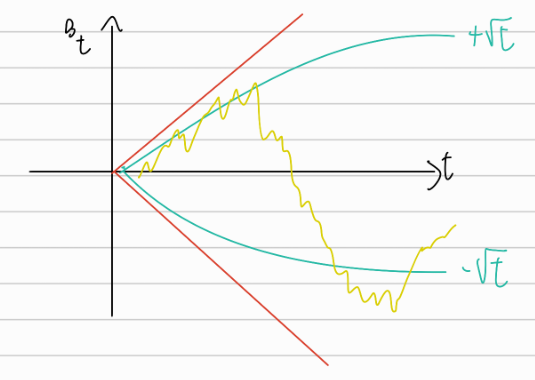
\includegraphics[width=0.5\linewidth]{img/screenshot043}
	\caption{Yes I know... The lines.}
	\label{fig:screenshot043}
\end{figure}
\begin{theorem}
	\emph{Le`vy 1937.} Let $B_{t}$ be a one-dimensional \bwm{}. Then
	\begin{equation*}
		\pr\left(\overline{\lim_{h\to0}}\frac{\sup|B_{t+h}-B_{t}|}{\sqrt{2h\ln \frac{1}{h}}}=1\right)=1.
	\end{equation*}
\end{theorem}
Note that $\sqrt{2h\ln\frac{1}{h}}$ is increasing in (0,$\frac{1}{e}$).
\begin{theorem}
	\emph{Law of iterated logarithm (Khinchin 1933)}. Let $B_{t}$ be a one-dimensional \bwm. Then
	\begin{equation*}
		\pr\left(\overline{\lim_{t\to\infty}}\frac{B_{t}}{\sqrt{2t\ln\ln t}}=1\right)=1.
	\end{equation*}
\end{theorem}
\begin{figure}[H]
	\centering
	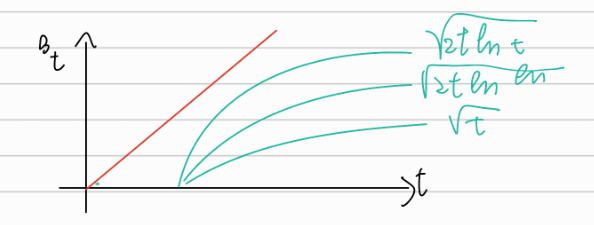
\includegraphics[width=0.5\linewidth]{img/screenshot044}
	\caption{I am sorry. The fucking homeworks are due soon.}
	\label{fig:screenshot044}
\end{figure}
\begin{corollary}
	Let $B_{t}$ be a one-dimensional \bwm. Then, a.s.,
	\begin{equation*}
		\begin{array}{cc}
			\varlimsup_{t\to\infty}\frac{B_{t}}{\sqrt{2t\ln\ln t}}=1&\varlimsup_{t\to0}\frac{B_{t}}{\sqrt{2t\ln\ln\frac{1}{t}}}=1\\
			\varliminf_{t\to\infty}\frac{B_{t}}{\sqrt{2t\ln\ln t}}=-1&\varliminf_{t\to0}\frac{B_{t}}{\sqrt{2t\ln\ln\frac{1}{t}}}=-1.
		\end{array}
	\end{equation*}
\end{corollary}
Define 
\begin{equation*}
	h(t)=\sqrt{2t\ln\ln t}.
\end{equation*}
For every $\varepsilon>0,\delta>0$, the \bwm{} $B_{t}$ is infinitely often in the region
\begin{equation*}
	\left\{(t,y):0\leq t\leq\delta\qquad(1-\varepsilon)h(t)\leq y\leq(1+\varepsilon)h(t)\right\}.
\end{equation*}
\begin{figure}[h]
	\centering
	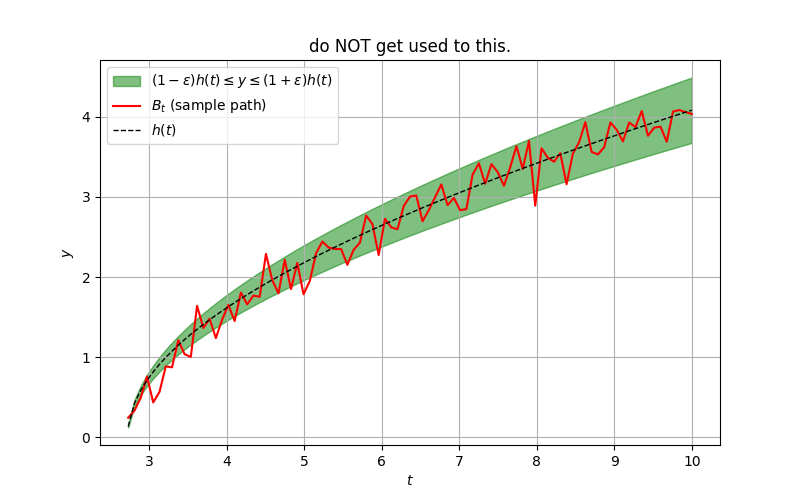
\includegraphics[width=0.6\linewidth]{img/screenshot045}
	\caption{FIRST and LAST time I use Matplotlib.}
	\label{fig:screenshot045}
\end{figure}
And also, infinitely often,
\begin{equation*}
	\left\{(t,y):0\leq t\leq\delta\qquad-(1+\varepsilon)n(t)<y<-(1-\varepsilon)h(t)\right\}.
\end{equation*}
\begin{figure}[h]
	\centering
	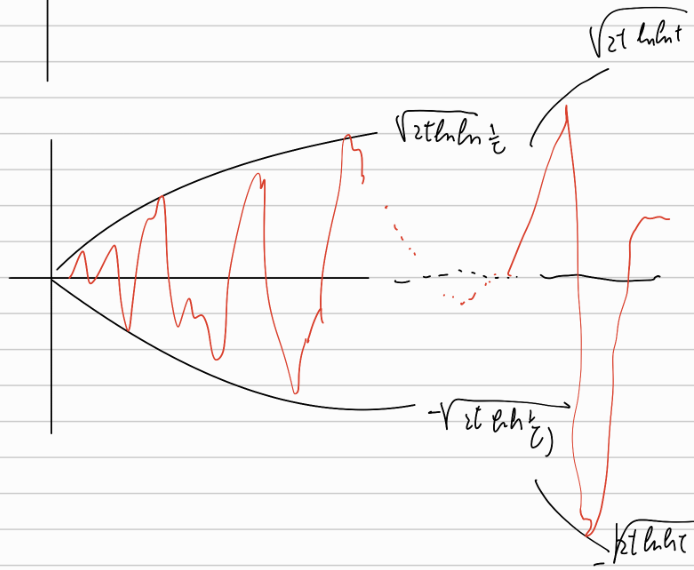
\includegraphics[width=0.4\linewidth]{img/screenshot046}
	\caption{Idk bruv she drew this thing but I don't even know what this is supposed to be in the first place.}
	\label{fig:screenshot046}
\end{figure}
\chapter{Diffusion processes}
\section{One-dimensional diffusion processes}
\subsection{Definition}
\begin{definition}
	Let $\{X(t)\}$ be a continuous time stochastic process such that:
	\begin{enumerate}
		\item its sample paths are continuous functions of $t$, a.s.;
		\item it has strong Markov property.
	\end{enumerate}
	Then $\{X(t)\}$ is called \emph{diffusion process}.
\end{definition}
Here we incur in a problem: while before we just took for granted that \bwm{} was continuous, now we need to \textit{actually define} what ``continuous'' means. But why should we care about diffusion processes?
\begin{enumerate}
	\item Many real world phenomena can be modeled through diffusion. We saw how \bwm{} can model the motion of particles, but if we want to take into account friction as well we need to use a diffusion process to model that behavior.
	\item For diffusions we are able to compute many useful functionals. So this is motivation to use them!
	\item Suitable rescaling allows us to approximate discrete time or space processes through diffusion processes. This is useful because for many discrete processes, as soon as combinatorics enter the stage the computations become a nightmare (think about a random walk with random step size... and think about considering all the various combinations of steps to reach a certain state).
\end{enumerate}
\begin{definition}
	The interval $I=(l,r)$ (or $[l,r)$ or $(l,r]$ or $[l,r]$) where we allow $l=-\infty$ and $r=+\infty$, is called \emph{diffusion interval}.
\end{definition}
\begin{definition}
	A stochastic process is said to be \emph{regular} if, starting from any point $x_{0}$ in the interval $I$, any other point $z$ interior to $I$ bay be attained with positive probability. This means, if 
	\begin{equation*}
		T_{z}=\inf\{t>0:X(t)>z|X(0)=x_{0}<z\},
	\end{equation*}
	then the process is regular if
	\begin{equation*}
		\pr(T_{z}<\infty|X(0)=x_{0})>0\qquad\every l<x_{0}<z<r.
	\end{equation*}
\end{definition}
\begin{figure}[H]
	\centering
	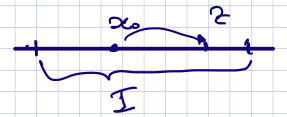
\includegraphics[width=0.5\linewidth]{img/screenshot047}
	\caption{Drawing from the one and only Professor herself.}
	\label{fig:screenshot047}
\end{figure}
We will consider only regular processes. For Markov processes we have
\begin{equation*}
	\lim_{h\to0}\frac{1}{h}\pr(|X(t+h)-X(t)|>\varepsilon|X(t)=x)=\lambda(x,\varepsilon)\geq0.
\end{equation*}
\begin{remark}
	For diffusion processes we have
	\begin{equation*}
		\lim_{h\to0}\frac{1}{h}\pr(|X(t+h)-X(t)|>\varepsilon|X(t)=x)=0.
	\end{equation*}
	This means that large displacements over small intervals are very unlikely.
\end{remark}\begin{definition}
A strong Markov process ${X(t)}$ is called \emph{standard prcoess} if its sample path verifies:
\begin{enumerate}
	\item $X_{\omega}(t)$ is right continuous:
	\begin{equation*}
		\lim_{t\to s}X(t)=X(s);
	\end{equation*}
	\item the left limit exists;
	\item $X(t)$ is continuous from the left through Markov (stopping) times. 
\end{enumerate}
\end{definition}
The third characteristic means that if $T_{1}<T_{2}<\ldots$ are stopping times then
\begin{equation*}
	\lim_{n\to\infty}X(T_{n})=X(T)
\end{equation*}
whenever $T<\infty$ a.s. So it is continuous on the left just by stopping times: this means, ultimately, that the only kind of discontinuity allowed in a standard process are (unpredictable) jumps.\par
For example, the Poisson process is standard.
\begin{proposition}
	Every strong Markov process continuous in probability and subject to ``mild conditions'' admits a standard version.
\end{proposition}
\subsection{The Dynkin condition}
We may now ask whether there are conditions to recognize if a standard process is also a diffusion. Clearly Poisson processes are not diffusions so we need a tool to restrict the class. This is the \emph{Dynkin condiition}:
\begin{equation*}
	\lim_{h\searrow0}\frac{1}{h}\pr(|X(t+h)-X(t)|>\varepsilon|X(t)=x)=0
\end{equation*}
where the convergences prevails uniformly for $x$ restricted to any compact sub-interval of $(l,r)$ and $t$ on any finite interval on $[0,N]$. \par
Since continuity of a process is tied to the increments, we should analyze them.
\begin{definition}
	Let $\Delta_{h}X(t)$ be the increment of the process $X(t)$ in an interval of size $h$.
\end{definition}
\begin{equation*}
	\Delta_{h}X(t)=(X(t-h))-X(t).
\end{equation*}
\begin{figure}[h]
	\centering
	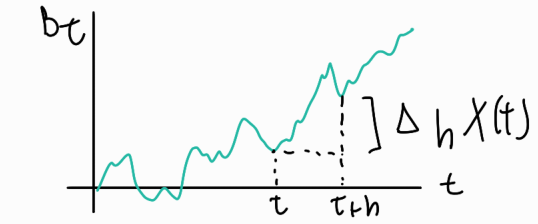
\includegraphics[width=0.5\linewidth]{img/screenshot048}
	\caption{It is hard to to think about the easy way out.}
	\label{fig:screenshot048}
\end{figure}
Then for $l<xL<r$ define
\begin{equation*}
	\lim_{h\searrow0}\frac{1}{h}\ev{\Delta_{h}X(t)|X(t)=x}=\mu(x,t)
\end{equation*}
as the \emph{drift} or \emph{infinitesimal mean} and
\begin{equation*}
	\lim_{h\searrow0}\frac{1}{h}\ev{\left(\Delta_{h}X(t)\right)^{2}|X(t)=x}=\sigma^{2}(x,t)
\end{equation*}
as the \emph{infinitesimal variance} of $X(t)$ or \emph{diffusion parameter}.
Keep in mind that the infinitesimal mean and variance are the mean and variance of the infinitesimal increment, not of the whole process!
\begin{remark}
	A diffusion process is characterized as having the following conditions:
	\begin{enumerate}
		\item it has strong Markov property;
		\item $\lim_{h\searrow0}\pr(|\Delta_{h}X(t)|>\varepsilon|X(t)=x)=0$, $x\in I$;
		\item $\mu(x,t)$ and $\sigma^{2}(x,t)$ are continuous functions of $x$ and $t$.
	\end{enumerate}
\end{remark}
This is equivalent to the Dynkin condition, but it is much easier to check: we are just asking that the probability of large increments for to zero with some conditions on the speed at which the process leaves the current state.
\begin{definition}
	If
	\begin{equation*}
		\begin{array}{c}
			\mu(x,t)=\mu(x)\\
			\sigma^{2}(x,t)=\sigma^{2}(x)
		\end{array}\every x,t
	\end{equation*}
	the process is said to be \emph{time homogeneous}.
\end{definition}
\begin{remark}
	Think about
	\begin{equation*}
		\ev{\Delta_{h}X(t)|X(t)=x}=\mu(x)h+o(h).
	\end{equation*}
	Moreover, the variance can be rewritten
	\begin{align*}
		\var\left[\Delta_{h} X(t)|X(t)=x\right]&=\ev{\left(\Delta_{h}X(t)\right)^{2}|X(t)=x}-\left(\ev{\Delta_{h}X(t)|X(t)=x}\right)^{2}\\
		&=\sigma^{2}(x)h+\underset{1}{o}(h)-\left(\mu(x)h+o(h)\right)^{2}\\
		&=\sigma^{2}(X)h+\underset{2}{o}(h)
	\end{align*}
	The different numbers under $o$ just means that those are different errors.
\end{remark}
\begin{definition}
	We define the infinitesimal moment of order $r$ as
	\begin{equation*}
		\lim_{h\searrow0}\frac{1}{h}\ev{\left(\Delta_{h}X(t)\right)^{r}|X(t)=x}\qquad r=3,4,\ldots
	\end{equation*}
	For diffurion processes these infinitesimal moments are zero for r>2.
\end{definition}
\begin{lemma}
	If a standard process satisfies
	\begin{equation*}
		\lim_{h\searrow0}\frac{1}{h}\ev{\left(\Delta_{h}X(t)\right)^{p}|X(t)=x}=0
	\end{equation*}
	for some $p>2$ uniformly for $x$ in an compact subinterval of $(l,r)$ and $t$ in any finite interval in $[0,N]$ then the Dynkin condition is verified.
\end{lemma}
\begin{fancyproof}
	Use Chebyshev:
	\begin{equation*}
		\frac{1}{h}\pr(|X(t+h)-X(t)|>\varepsilon|X(t)=x)\leq\frac{\ev{|\Delta_{h}X(t)}|^{p}|X(t)=x}{h\varepsilon^{p}}.
	\end{equation*}
\end{fancyproof}
\subsection{Characterization of Diffusion processes}
We can define a diffusion process:
\begin{enumerate}
	\item In terms of infinitesimal coefficients:
	\begin{equation*}
		\begin{array}{c}
			\mu(x,t)\\
			\sigma^{2}(x,t)\\
			I\text{ (diffusion interval)}
		\end{array}
	\end{equation*}
	We should also specify, for example, the behavior at the boundaries of $I$: it could be an absorbing boundary or some other shit.
	Think about a \bwm{} on $I(-\infty,\infty]$: depending on whether 0 is absorbing we have two different sample paths.
	\begin{figure}[H]
		\centering
		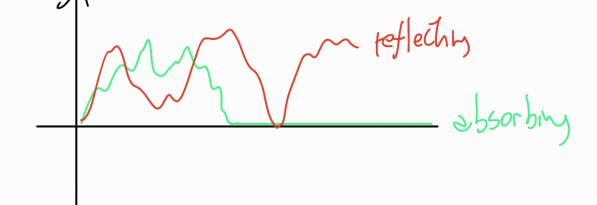
\includegraphics[width=0.5\linewidth]{img/screenshot049}
		\caption{The ``internal'' law of movement remains the same and so do the diffuson paramenters. Of course, this is until the process attains 0.}
		\label{fig:screenshot049}
	\end{figure}
	\item We have an alternative definition using stochastic differential equations:
	\begin{equation*}
		\begin{cases}
			\dif X_{t}=\mu(X_{t},t)\dt+\sigma(X_{t},t)\dif B_{s}\\
			X_{0}=c
		\end{cases}
	\end{equation*}
	This is of course just notation. $\dif B_{s}$ doesn't make sense as a concept because the Brownian motion doesn't admit derivative! This notation actually means
	\begin{equation*}
		X_{t}=c+\ubracketthin{\int_{t_{0}}^{t}\mu(X_{s},s)\ds}_{\claptext{normal Riemann}}+\ubracketthin{\int_{t_{0}}^{t}\sigma(X_{s},s)\dif B_{s}}_{\claptext{Ito integral...}}
	\end{equation*}
	We will need a new type of integral to deal with this shit: the Ito integral. Which is bad and stupid.
	\item We can use martingales and, in particular, the \emph{Storook-Varadhan} martingale. We do not care.
\end{enumerate}
A diffusion process which is often used is the \emph{Orstein-Uhlenbeck} process:
\begin{equation*}
	I=(-\infty,+\infty),\;\begin{cases}
		\mu(x)=-\alpha(x)\\
		\sigma^{2}(x)=\sigma^{2}
	\end{cases}
\end{equation*}
Where $\alpha>0$, $\sigma>0$ are arbitrary. This gives us the following stochastic differential equation:
\begin{equation*}
	\dif X_{t}=-\alpha X_{t}\dt+\sigma\dif B_{t}.
\end{equation*}
Not considering the noise (that in this model is represented by the \bwm{} component) we describe the phenomenon as a simple first order differential equation that we can quite easily solve. Then we add pack the noise (that contains all stochastic elements) and so we have our perturbed model.\par
There are other methods to ``build'' new diffusions.
\begin{theorem}
	Let $X(t)$ be a regular diffusion process on $I=(\lambda,r)$ (it bakes no difference open or closed). Let $\mu(x)$ and $\sigma^{2}(x)$ be its infinitesimal moments. Let $g(x)$ be a strictly monotone function on $I$ with continuous first and second derivatives $g'(x)$ and $g''(x)$ for $x\in(l,r)$. Then the transformed process
	\begin{equation*}
		Y(t)=g(X(t))
	\end{equation*}
	is a regular diffusion process on $(g(l),g(r))$ and
	\begin{equation*}
		\begin{array}{c}
			\mu_{Y}(y)=\unmezz\sigma^{2}(x)g''(x)+\mu(x)g'(x)\big|_{x=g^{-1}(y)}\\
			\sigma^{2}_{Y}(y)=\sigma^{2}(x)g'(x)\big|_{x=g^{-1}(g)}
		\end{array}
	\end{equation*}
	Where $y=g(x)$.
\end{theorem}
\begin{fancyproof}
	Let $g$ be strictly increasing and twice continuously differentiable. Take the Taylor expansion (this is a classic way of dealing with these things)
	\begin{equation*}
		g(x+\Delta X)=g(x)+\Delta Xg'(x)=\frac{(\Delta X)^{2}}{2}g''(x)+\unmezz(\Delta X)^{2}\left[g''(\xi)-g''(x)\right]
	\end{equation*}
	for $x\leq\xi<x+\Delta X$. Substitute 
	\begin{equation*}
		\begin{array}{c}
			x\to X(t)\\
			\Delta  x\to\Delta X_{h}(t)
		\end{array}
	\end{equation*}
	So we get 
	\begin{align*}
		g(X(t+h))&=g(X(t))+\Delta X_{h}g'(X(t))+\frac{(\Delta X_{h})^{2}}{2}g''(X(t))+\\
		&+\frac{(\Delta X_{h})^{2}}{2}\left[g''(\xi(\omega))-g''(X(t))\right].
	\end{align*}
	Here $X(t)\leq\xi(\omega)\leq X(t+h)$: $\xi$ ha an $\omega$ as argument because it is now a random variable. Substitute $Y(t)$:
	\begin{align*}
		Y(t+h)-Y(t)=&\Delta_{h} X g'(X(t)+\unmezz(\Delta_{h})^{2}g''(X(t)))+\\&+\frac{(\Delta X)^{2}}{2}\cdot\left[g''(\xi(\omega))-g''(X(t))\right]\qquad\text{for }g(X(t))=Y(t).
	\end{align*}
	Now:
	\begin{enumerate}
		\item condition on $Y(t)=y$ (which means $X(t)=x$, $g(X(t))=Y(t)=y$);
		\item take the expectation;
		\item divide by $h$ and take the limit:
		\begin{align*}
			\lim_{h\searrow0}\frac{1}{h}&\ev{Y(t-h)-Y(t)|Y(t)=y}=\mu(x)g'(X(t))+\frac{\sigma^{2}(x)}{2}g''(X(t))+\\
			&+\unmezz\lim_{h\searrow0}\frac{1}{h}\ev{g''(\xi(\omega))-g''(X(t))|Y(t)=y}\quad\text{with }X(t)=g^{-1}(Y(t)).
		\end{align*}
	\end{enumerate}
	We know that $g''(x)$ is continuous, so 
	\begin{equation*}
		g''(\xi(\omega))\to g''(X(t))
	\end{equation*}
	and therefore
	\begin{equation*}
		\mu_{Y}(y)=\lim_{h\searrow0}\ev{Y(t+h)-Y(t)|Y(t)=y}=\mathcolor{OliveDrab4}{\mu(x)g'(x)+\frac{\sigma^{2}(x)}{2}g''(x)\big|_{x=g^{-1}(y)}}.
	\end{equation*}
	We still need to prove that the diffusion parameter is equal to the one in the hypothesis. We know that
	\begin{equation*}
		Y(t+h)-Y(t)=\Delta X g'(X(t))+\unmezz(\Delta X)^{2}g''(X(t))+\unmezz(\Delta X)^{2}\cdot[g''(\xi(\omega))+g''(X(t))]
	\end{equation*}
	and this means that 
	\begin{equation*}
		\left[Y(t+h)-Y(t)\right]^{2}=(\Delta X)^{2}(g(X(t)))^{2}+R_{h}
	\end{equation*}
	where $R_{h}$ contains only $(\Delta X)^{3}$ and higher order terms: this makes them vanish faster than $(\Delta X)^{2}$, making them negligible as $h\searrow0$:
	\begin{equation*}
		\lim_{h\searrow0}\frac{1}{h}\ev{(Y(t+h)-Y(t))^{2}|Y(t)=y}=\sigma^{2}(y)\left(g'(y)\right)^{2}
	\end{equation*}
	because we know that
	\begin{equation*}
		\lim_{h\searrow0}\frac{1}{h}\ev{|\Delta X|^{r}|X(t)=x}=0\qquad\every r\geq 3.
	\end{equation*}
	The condition
	\begin{equation*}
		\lim_{h\searrow0}\frac{1}{h}\pr(|X(t+h)-x|>\varepsilon|X(t)=x)=0
	\end{equation*}
	can be verified also for $Y(t)=g(X(t))$. This means (??? Thank you Zucca) that $Y(t)$ is a diffusion process with infinitesimal parameters as the one stated in the thesis.
\end{fancyproof}
\subsection{Examples of transformed diffusion processes}
An example of transformed process is the \emph{Lamperti transform}:
\begin{equation*}
	g(x)=\int^{x}\frac{1}{\sigma_{X}(z)}\dz.
\end{equation*}
This is very useful\footnote{Of course, not in an \textit{actual} sense.} because it allows us to transform any diffusion into a diffusion with constant diffusion parameter, which is much easier to handle. Indeed, the parameters are
\begin{align*}
		\sigma^{2}_{Y}(y)&=\sigma^{2}_{X}(x)\cdot\frac{1}{\sigma^{2}}_{X}(x)=1\\
		\mu_{Y}(y)&=\unmezz\sigma^{2}_{X}(x)\frac{\dif}{\dx}\left(\frac{1}{\sigma_{X}(x)}\right)+\frac{\mu_{X}(x)}{\sigma_{X}(x)}\Big|_{y=g(x)}.
\end{align*}
So all the dependency is conveniently contained in the infinitesimal mean.
\begin{remark}
	The meaning of $\mu_{Y}(y)$ is to capture the drift, or deterministic behavior, of the process while $\sigma^{2}_{Y}(y)$ is a noise component.
	We can also use this fact inside the stochastic differential equation:
	\begin{equation*}
		\begin{cases}
			\dif X_{t}=\ubracketthin{\mu(t,X_{t})\dt}_{\text{deterministic function}}+\ubracketthin{\sigma(t,X_{t})\dif B_{t}}_{\text{noise that could involve the process itself}}\\
			X_{0}=x_{0}.
		\end{cases}
	\end{equation*}
\end{remark}
Never forget that this is just ugly notation for
\begin{equation*}
	X_{t}=X_{0}+\int_{0}^{t}\mu(s,X_{s})\ds+\int_{0}^{t}\sigma(s,X_{s})\dif B_{s}
\end{equation*}
(yes I know, it's a little bit different than above but it is because we switched professor, be a big boy about it) because technically it doesn't make sense to say $\dif B_{s}$ since you can't differentiate \bwm. The integral notation holds because we define a new object, the Ito integral, just to make sense for this setting. If $\sigma^{2}$ is continuous is like a Riemann integral, otherwise shit happens.\par
Another example of transformed process is the \emph{geometric \bwm}:
\begin{definition}
	Let ${(X_{t})}_{t\geq 0}$ be a \bwm{} with drift $\mu$ and diffusion coefficient $\sigma^{2}$ (remember that $\sigma$ is present in the definition of \bwm{} with drift?). The the process 
	\begin{equation*}
		Y(t)=e^{X(t)}
	\end{equation*}
	is called \emph{geometric \bwm{}} with $I=(0,\infty)$.
\end{definition}
This is not anymore a Gaussian process, but it is enough to take its log to go back to the normal \bwm. This is often used to model prices of assets traded in a perfect market because it is non negative and it exhibits a long-term exponential growth or decay. We know that
\begin{align*}
	y&=g(x)=e^{x}\\
	g'(x)&=g''(x)=e^{x}=y
\end{align*}
so using the theorem above we know that
\begin{align*}
	\mu_{Y}(y)&=\left(\mu+\unmezz\sigma^{2}\right)y\\
	\sigma^{2}(y)&=\sigma^{2}y^{2}.	
\end{align*}
We can plug this into our SDE:
\begin{equation*}
	\dif Y_{t}=\left(\mu+\unmezz\sigma^{2}\right)Y_{t}\dt+\sigma Y_{t}\dif B_{t}.
\end{equation*}
The interesting thing to note here is that while the process is exponential, the coefficients of the SDE are linear. This tells us how batshit insane the variability of this thing is. If the coefficient was squared we would already be having a very unpleasant time trying to solve this SDE in closed form.\par
Another useful example is the \emph{Bessel process}. It is the euclidean distance from the origin of an n-dimensional \bwm.
\begin{equation*}
	Y(t)=\sqrt{\ubracketthin{X_{1}(t)^{2}+\ldots+X_{n}(t)^{2}}_{\claptext{components of $n$-dim. BM}}}
\end{equation*}
We want to compute the infinitesimal parameters. We need two steps. 
\begin{enumerate}
	\item Define
	\begin{equation*}
		Z(t)=X_{1}(t)^{2}+\ldots+X_{n}(t)^{2}
	\end{equation*}
	where ${\{X_{i}(t)\}}_{t\geq0}$ are independent \bwm{} processes. We condition on $X_{i}(t)=x_{i}$ for $i=1,\ldots,n$ and we write
	\begin{equation*}
		\begin{array}{>{\displaystyle}c}
			X_{i}(t+\Delta t)=x_{i}+\Delta X_{i}\\
			Z_{i}(t+\Delta t)=z+\Delta Z
		\end{array}
	\end{equation*}
	where $z=x_{1}^{2}+\ldots+x_{n}^{2}$. We know that
	\begin{align*}
		\Delta Z&=Z(t+\Delta t)-Z(t)\\
		&=\ubracketthin{[X_{1}(t+\Delta t)]^{2}}_{(x_{1}+\Delta X_{1})^{2}}-x_{1}^{2}+\ldots+[X_{n}(t+\Delta t)]^{2}-x^{2}_{n}\\
		&=2(x_{1}\Delta X_{1}+\ldots+x_{n}\Delta X_{n})+\left[(\Delta X_{1})^{2}+\ldots+(\Delta X_{n})^{2}\right].
	\end{align*}
	We know that $\Delta X_{1},\ldots,\Delta X_{n}$ are i.i.d. $\distnorm{0,\Delta t}$.
	So we know that
	\begin{equation*}
		\ev{\Delta Z|Z(t)=z}=n\Delta t
	\end{equation*}
	and
	\begin{equation*}
		\ev{(\Delta Z)^{2}|Z(t)=z}=4\left(\sum_{i=1}^{n}x_{i}^{2}\right)\Delta t+o(\Delta t)
	\end{equation*}
	where $o(\Delta t)$ contains terms of order $(\Delta X)^{4}$ or higher. Moreover the fourth moment is
	\begin{equation*}
		\ev{(\Delta Z)^{4}|Z(t)=z}=o\left(\left(
		\Delta t\right)^{2}\right)
	\end{equation*}
	So the lemma condition holds for $p=4$. This means that ${\{Z(t)\}}_{t\geq0}$ is a diffusion with 
	\begin{align*}
		\mu(z)&=n\\
		\sigma^{2}(z)&=4z.
	\end{align*}
	\item The Bessel process is:
	\begin{equation*}
		Y(t)=\sqrt{Z(t)}
	\end{equation*}
	so we can set
	\begin{equation*}
		\begin{array}{>{\displaystyle}c}
			g(z)=\sqrt{z}\\
			g'(z)=\frac{1}{2\sqrt{z}}=\frac{1}{2y}\\
			g''(z)=-\frac{1}{4z^{\sfrac{3}{2}}}=-\frac{1}{4y^{3}}.
		\end{array}
	\end{equation*}
	We can now apply the theorem to get the infinitesimal moments:
	\begin{equation*}
		\begin{array}{>{\displaystyle}c}
			\mu_{Y}(y)=\frac{n-1}{2y}\\
			\sigma^{2}_{Y}(y)=1.
		\end{array}
	\end{equation*}
	Plugging this into the SDE we get
	\begin{equation*}
		\dif Y_{t}=\frac{n-1}{2Y_{t}}\dif t+\dif B_{t}.
	\end{equation*}
	If $n=1$ we get
	\begin{equation*}
		\left\{\begin{array}{*2{>{\displaystyle}c}}
			\mu_{Y}(y)=0&\text{reflecting \bwm}\\
			\sigma^{2}_{Y}=1&I=[0,\infty).
		\end{array}\right.
	\end{equation*}
\end{enumerate}
\section{Kolmogorov backward and forward equations}
Let $\{X_{t},t\geq 0\}$ be a regular, time homogeneous diffusion process on $I=(l,r)$. Let
\begin{equation*}
	F(y,t|x,0)=\pr(X(t)<y|X(0)=x)
\end{equation*}
be the transition \textit{distribution} function of $X(t)$ with initial condition
\begin{equation*}
	F(y,0|x,0)=\begin{cases}
		1&\text{if }x\leq y\\
		0&\text{if }x>y.
	\end{cases}
\end{equation*}
Let us assume that $F(y,t|x,0)$ has density on $I$:
\begin{equation*}
	f(y,t|x,0)=\frac{\dif}{\dt}F(y,t|x,0)
\end{equation*}
which is the transition \textit{density} function.
\subsection{Kolmogorov backward differential equation}
We want to derive a partial differential equation for 
\begin{equation*}
	u(t,x)=\ev{g(X(t))|X(0)=x}
\end{equation*}
where $g(x)$ is a bounded and piecewise continuous function on $I$. We will see that $u(t,x)$ satisfies
\begin{equation}
	\frac{\partial u}{\partial t}=\unmezz\sigma^{2}(x)\frac{\partial^{2}u}{\partial x^{2}}+\mu(x)\frac{\partial u}{\partial x}\tag*{\faPastafarianism}\label{pasta}
\end{equation}
with $u(0^{+},x)=\lim_{h\searrow0} u(h,x)=g(x)$. The particular case
\begin{equation*}
	g(\eta)=\begin{cases}
		1&\text{if }\eta\leq y\\
		0&\text{if }\eta>y
	\end{cases}
\end{equation*}
gives
\begin{equation*}
	u(t,x)=\ev{\indi_{\{X(t)\leq y\}}|X(0)=x}=F(y,t|x,0)
\end{equation*}
and \ref{pasta} becomes the \emph{Kolmogorov backward equation}:
\begin{equation*}
	\frac{\partial F(y,t|x,0)}{\partial t}=\unmezz\sigma^{2}(x)\frac{\partial^{2}F(y,t|x,0)}{\partial x^{2}}+\mu(x)\frac{\partial F(y,t|x,0)}{\partial x}\tag*{\faBackward}\label{bward}
\end{equation*}for $t>0,l<x,y>r$ and with initial conditions
\begin{equation*}
	F(y,0^{+}|x,0)=\begin{cases}
		1&\text{if }x\leq y\\
		0&x>y.
	\end{cases}
\end{equation*}
Also, the transition density function $f(y,t|x,0)$ satisfies the Kolmogorov backward equation
\begin{equation*}
	\frac{\partial f(y,t|x,0)}{\partial t}=\mu(x)\frac{\partial f(y,t|x,0)}{\partial x}=\unmezz\sigma^{2}(x)\frac{\partial^{2}f(y,t|x,0)}{\partial x^{2}}\tag*{\faBackspace}\label{backspace}
\end{equation*}
for $t>0$, $l<x,y<r$.
\begin{remark}
	The solution of \ref{bward} and \ref{backspace} in general is not unique.
\end{remark}
\begin{figure}[H]
	\centering
	\includegraphics[width=0.7\linewidth]{img/screenshot050}
	\caption{On the left, \bwm{} with absorbing boundary; on the right, with reflecting boundary.}
	\label{fig:screenshot050}
\end{figure}
Both of the \bwm s in figure \ref{fig:screenshot050} satisfy \ref{bward} and \ref{backspace} but they are clearly different things. We need to add information on the behavior of the process around the boundaries. This is because to find the solution we should add the boundary conditions.
\begin{fancyproof}
	It is difficult to prove that $F,f,u$ are differentiable in $t$ and twice differentiable in $x$ so we start from these hypotheses and we prove that $f(y,t|x,0)$ satisfies \ref{backspace}.\par
	We know that the transition density function $f$ satisfies the \emph{Chapman-Kolmogorov/Smoluchowski} equation
	\begin{equation*}
		f(x,t|x_{0},t_{0})=\int_{I}f(x,t|y,\tau)f(y,\tau|x_{0}|t_{0})\dy.\tag*{\faWalking}\label{walking}
	\end{equation*}
	\begin{figure}[H]
		\centering
		\includegraphics[width=0.7\linewidth]{img/screenshot051}
		\caption{I didn't manage to draw this myself because at this point I had largely fallen asleep in the classroom.}
		\label{fig:screenshot051}
	\end{figure}
	We consider the \ref{walking} equation with
	\begin{equation*}
		\begin{array}{c}
			t_{0}\leq\tau<t\\
			x=X(t)\\
			y=X(\tau)\\
			x_{0}=X(t_{0}).
		\end{array}
	\end{equation*}
	After substituting $t_{0}$ with $t_{0}-\Delta t$ and $\tau$ with $t_{0}$ the equation \ref{walking} becomes
	\begin{equation*}
		f(x,t|x_{0},t_{0}-\Delta t)=\int_{I}f(x,t|y,t_{0})f(y,t_{0}|x_{0},t_{0}-\Delta t)\dy
	\end{equation*}
	where 
	\begin{equation*}
		\begin{array}{l}
			x=X(t)\\
			x_{0}=X(t_{0}-\Delta t)\\
			y=X(t_{0})\\
			\Delta t\text{ is a small increment}.
		\end{array}
	\end{equation*}
	We subtract
	\begin{equation*}
		\mathcolor{Aquamarine4}{f(x,t|x_{0},t_{0})}=\mathcolor{Gold4}{\int_{I}}\mathcolor{Aquamarine4}{f(x,t|x_{0},t_{0})}\mathcolor{Gold4}{f(y,t|x_{0},t_{0}-\Delta t)\dy}
	\end{equation*}
	where the \textcolor{Gold4}{yellow} part integrates to 1. 
	\begin{align*}
		f(x,t|x_{0},t_{0}-\Delta t)-f(x,t|x_{0},t_{0})&=\int_{I}f(y,t_{0}|x_{0},t_{0}-\Delta t)\cdot\\
		&\cdot[f(x,t|y,t_{0})-f(x,t|x_{0},t_{0})]\dy\\
		&=\sum_{n=1}^{\infty}\int_{I}f(y,t_{0}|x_{0},t_{0}-\Delta t)\cdot\\
		&\ubracketthin{\cdot\frac{\partial^{n}f(x,t|x_{0},t_{0})}{\partial x_{0}^{n}}\frac{(y-x_{0})^{n}}{n!}}_{\claptext{Taylor series in $x_{0}$}}\dy.
	\end{align*}
	Now divide by $(-\Delta t)$ and let $\Delta t\to0$ so that
	\begin{equation*}
		\frac{\partial f(x,t|x_{0}|t_{0})}{\partial t_{0}}=-\sum^{\infty}_{n=1}\frac{1}{n!}\frac{\partial^{n}f(x,t|x_{0},t_{0})}{\partial x^{n}_{0}}\ubracketthin{\lim_{\Delta t\searrow0}\frac{1}{\Delta t}\int_{I}(y-x_{0})^{n}f(y,t_{0}|x_{0},t_{0}-\Delta t)\dy}_{A_{n}(x_{0},t_{0})}
	\end{equation*}
	where $A_{n}(x_{0},t_{0})$ are the infinitesimal moments of a diffusion process
	\begin{equation*}
		\lim_{h\searrow0}\frac{1}{h}\ev{|\Delta_{h}X(t)|^{n}|X(t)=x}.
	\end{equation*}
	We know that
	\begin{enumerate}
		\item $A_{1}(x_{0},t_{0})=\mu(x_{0},t_{0})$;
		\item $A_{2}(x_{0},t_{0})=\sigma^{2}(x_{0},t_{0})$;
		\item $A_{k}(x_{0},t_{0})=0$ for $\every k\geq3$.
	\end{enumerate}
	Then
	\begin{equation*}
		-\frac{\partial f}{\partial t_{0}}=\mu(x_{0},t_{0})\frac{\partial f}{\partial x_{0}}+\frac{\sigma^{2}(x_{0},t_{0})}{2}\frac{\partial^{2}f}{\partial x_{0}^{2}}.
	\end{equation*}
	If the process is time-homogeneous then we have that
	\begin{equation*}
		\begin{array}{c}
			f(x,t|x_{0},t_{0})=f(x,t-t_{0}|x_{0},0)\\
			A_{n}(x_{0},t_{0})=A_{n}(x_{0})\quad\every n.
		\end{array}\implies\frac{\partial f}{\partial t}=-\frac{\partial f}{\partial t_{0}}
	\end{equation*}
	and therefore
	\begin{equation*}
		\frac{\partial f}{\partial t}=\mu(x_{0})\frac{\partial f}{\partial x_{0}}+\frac{\sigma^{2}(x_{0})}{2}\frac{\partial^{2}f}{\partial x_{0}^{2}}.
	\end{equation*}
\end{fancyproof}
\subsection{Kolmogorov forward differential equation}
This is also called \emph{Fokker-Plank} equation\footnote{Fokker? I hardly know her.}. This is the dual of the \ref{bward} equation. It is the following:
\begin{equation*}
	\frac{\partial f}{\partial x}=-\frac{\partial}{\partial x}[\mu(x,t)f]+\frac{\partial^{2}}{\partial x^{2}}\left[\frac{\sigma^{2}(x,t)}{2}f\right]\tag*{\faForward}\label{fwd}
\end{equation*}
where $f$ is $f(x,t|x_{0},t_{0})$. \par
This equation seems more complex because $\mu$ multiplies $f$ and because we have second order derivatives. We have to note that here we are differentiating with respect to \textit{forward space} $x$ while before we were taking into account the starting point at time 0. We won't prove this result, but we need to use the Chapman-Kolmogorov equation with
\begin{equation*}
	\begin{array}{l}
		t\leadsto t+\Delta t\\
		\tau\leadsto t.
	\end{array}
\end{equation*}
We see some examples of application.
\begin{enumerate}
	\item \textit{General \bwm}. We know that the \bwm{} is time-homogeneous. Recall the \ref{bward} equation that in this case is:
	\begin{equation*}
		\frac{\partial f}{\partial t}=\frac{\sigma^{2}}{2}\frac{\partial^{2}f}{\partial x_{0}}\qquad I=(-\infty,+\infty).
	\end{equation*}
	This is the classical heat equation. We can prove that the result is the following:
	\begin{equation*}
		f(x,t|x_{0},t_{0})=\frac{1}{\sqrt{2\pi\sigma^{2}(t-t_{0})}}\expg{-\frac{(x-x_{0})^{2}}{2\sigma^{2}(t-t_{0})}}
	\end{equation*}
	and this is none other than then solution to the \ref{bward} equation. The system that gives us this solution is:
	\begin{equation*}
		\parbox{3cm}{\textcolor{SpringGreen3}{Cauchy\\Problem}}\begin{cases}
			\frac{\partial f}{\partial t}=\frac{\sigma^{2}}{2}\frac{\partial^{2}f}{\partial x_{0}^{2}}\\
			\lim_{t\to t_0}f(x,t|x_{0},t_{0})=\ubracketthin{\delta(x-x_{0})}_{\claptext{Dirac funct.}}&\text{\textcolor{SpringGreen2}{initial condition}}\\
			\lim_{|x|\to\infty}f(x,t|x_{0},t_{0})=\lim_{|x|\to\infty}\frac{\partial f}{\partial x}=0&\text{\textcolor{SpringGreen2}{boundary condition}}
		\end{cases}
	\end{equation*}
	The boundary condition specifies what happens at the boundaries of the diffusion interval, that in this case are $-\infty$ and $+\infty$. This is just an analytical problem: this has the advantage that we can basically forget about probability and other similar things.
	\item \textit{Reflected \bwm{} with boundary $a$}. We said that the Kolmogorov equation is the same for different processes, if we don't specify the boundaries. But how can we modify the system of equations to have a reflecting boundary? Recall \ref{fwd} equation. The transition probability density function $f^{+}(x,t|x_{0},t_{0})$ satisfies
	\begin{equation*}
		\frac{\partial f^{+}}{\partial t}=\frac{\sigma^{2}}{2}\frac{\partial^{2}f^{+}}{\partial x^{2}}\qquad I=(-\infty,a).
	\end{equation*}
	This seems equal to the \ref{bward} equation but just because the coefficients are constants.
	\begin{figure}[H]
		\centering
		\includegraphics[width=0.5\linewidth]{img/screenshot052}
		\caption{Do we really need this?}
		\label{fig:screenshot052}
	\end{figure}
	We know that
	\begin{equation*}
		\int_{-\infty}^{a}f^{+}(x,t|x_{0},t_{0})\dx=1
	\end{equation*}
	because all the mass of the motion is below $a$. We take the derivative with respect to time:
	\begin{equation*}
		\int_{-\infty}^{a}\frac{\partial f^{+}}{\partial t}\dx=0
	\end{equation*}
	but I know from the \ref{fwd} equation that $\frac{\partial f^{+}}{\partial t}=\frac{\sigma^{2}}{2}\frac{\partial^{2}f^{+}}{\partial x^{2}}$ so we can substitute and get
	\begin{equation*}
		\int_{-\infty}^{a}\frac{\sigma^{2}}{2}\frac{\partial^{2}f^{+}}{\partial x^{2}}\dx=\frac{\sigma^{2}}{2}\frac{\partial^{2}f^{+}}{\partial x^{2}}\bigg|_{-\infty}^{a}=0.
	\end{equation*}
	So the boundary condition for a reflecting boundary is
	\begin{equation*}
		\frac{\partial f^{+}}{\partial x}\bigg|_{x=a}=0.
	\end{equation*}
	The system becomes
		\begin{equation*}\begin{cases}
			\frac{\partial f^+}{\partial t}=\frac{\sigma^{2}}{2}\frac{\partial^{2}f^+}{\partial x_{0}^{2}}&\parbox{1cm}{$x<a$ $t>0$}\\
			\lim_{t\to t_0}f^{+}(x,t|x_{0},t_{0})=\ubracketthin{\delta(x-x_{0})}_{\claptext{Dirac funct.}}&\text{\textcolor{SpringGreen2}{initial condition}}\\
				\frac{\partial f^{+}}{\partial x}\bigg|_{x=a}=0&\text{\textcolor{SpringGreen2}{upper bound}}\\
			\lim_{x\to\infty}f^{+}(x,t|x_{0},t_{0})=\lim_{x\to\infty}\frac{\partial^{+} f}{\partial x}=0&\text{\textcolor{SpringGreen2}{lower bound}}
		\end{cases}
	\end{equation*}
	\item \textit{\bwm{} with absorbing boundary $a$}. The transition probability density function $\overline{f}(x,t|x_{0},t_{0})$ satisfies \ref{fwd}:
	\begin{equation*}
		\frac{\partial\overline{f}}{\partial t}=\frac{\sigma^{2}}{2}\frac{\partial^{2}\overline{f}}{\partial x^{2}}.
	\end{equation*}
	\begin{figure}[H]
		\centering
		\includegraphics[width=0.5\linewidth]{img/screenshot053}
		\caption{No, we don't.}
		\label{fig:screenshot053}
	\end{figure}
	The integral of the density will be lower than 1! This is because everything is concentrated in $a$ which being a point has probability 0:
	\begin{equation*}
		\int_{-\infty}^{a}\overline{f}(x,t|x_{0},t_{0})\dx<1.
	\end{equation*}
	\begin{figure}[h]
		\centering
		\includegraphics[width=0.5\linewidth]{img/screenshot054}
		\caption{This is a mixed distribution of continuous and discrete and it is ``incomplete''!}
		\label{fig:screenshot054}
	\end{figure}
	The system becomes
		\begin{equation*}\begin{cases}
			\frac{\partial\overline{f}}{\partial t}=\frac{\sigma^{2}}{2}\frac{\partial^{2}\overline{f}}{\partial x_{0}^{2}}&\parbox{1cm}{$x<a$ $t>0$}\\
			\lim_{t\to t_0}\overline{f}(x,t|x_{0},t_{0})=\ubracketthin{\delta(x-x_{0})}_{\claptext{Dirac funct.}}&\text{\textcolor{SpringGreen2}{initial condition}}\\
			\overline{f}(x,t|x_{0},t_{0})=0&\text{\textcolor{SpringGreen2}{lower bound}}\\
			\lim_{x\to\infty}\overline{f}(x,t|x_{0},t_{0})=\lim_{|x|\to\infty}\frac{\partial \overline{f}}{\partial x}=0&\text{\textcolor{SpringGreen2}{upper bound}}
		\end{cases}\tag*{\faBezierCurve}\label{bezier}
	\end{equation*}
	\item \textit{\bwm{} with absorbing boundary $a>0$}. Let us denote $\{\overline{B}(t),t\geq0\}$ as the \bwm{} with absorbing boundary $a$. Let
	\begin{equation*}
		T_{a}:=\inf\{t>B(t)\}
	\end{equation*}
	be the first passage time through $a$. We want to define
	\begin{equation*}
		\overline{B}(t)=\begin{cases}
			B(t)&\text{if }t<T_{a}\\
			a&\text{if }f\geq T_{a}.
		\end{cases}
	\end{equation*}
	We want to find the transition density function of $\overline{B}(t)$, that is
	\begin{equation*}
		\pr\left(\overline{B}(t)\leq y\right)\qquad\text{which is short for }\pr\left(\overline{B}(t)\leq y|B(0)=0\right).
	\end{equation*}
	The aim here is to express it in terms of the normal \bwm{} $B(t)$. We know that
	\begin{align*}
		\pr\left(\overline{B}(t)\leq y\right)&=\pr(B(t)\leq y,T_{a}>t)\qquad y<a\\
		&=\pr(B(t)\leq y)-\pr(B(t)\leq y, T_{a}<t)\scriptscriptstyle\qquad\text{because }\pr(A)=\pr(A\cap B)+\pr(A\cup B^{c})\\
		&=\pr(B(t)\leq y)-\pr\left(B(t)\leq y\max_{0\leq s\leq t}B(s)\geq a\right)\\
		&=\pr(B(t)\leq y)-\pr(B(t)\geq 2a-y)\qquad\scriptscriptstyle\text{refl. principle}\\
		&=\pr(B(t)\leq y)-[1-\pr(B(t)<2a-y)]
	\end{align*}
	so then transition density function is
	\begin{align*}
		\overline{f}_{a}(t,y|0,0)&=f(t,y|0,0)-f(t,y|0,2a)\\
		&=\ubracketthin{\frac{1}{\sqrt{2\pi t}}e^{-\frac{y^{2}}{2t}}-\frac{1}{\sqrt{2\pi t}}e^{-\frac{(y-2a)^{2}}{2t}}}_{\leq 1\text{ as expected!}}.
	\end{align*}
	I basically delete from the normal transition density function $f(t,y|0,0)$ all trajectories that are ``not acceptable'' and for the reflection principle they happen to equivalent to all the trajectories that start from $2a$! This is very cool and it is a neat trick to solve the system \ref{bezier}. We could do this only because the \bwm{} has the reflection property... and this is not a common thing.
	\item \textit{\bwm{} with reflecting boundary $a>0$}. Define $\{B^{+}(t),t\geq0\}$ as the \bwm{} with reflecting boundary $a>0$:
	\begin{equation*}
		B^{+}(t)=\begin{cases}
			B(t)&\text{if }B(t)\leq a\\
			2a-B(t)&\text{if }B(t)>a.
		\end{cases}
	\end{equation*}
	\begin{figure}[h]
		\centering
		\includegraphics[width=0.5\linewidth]{img/screenshot055}
		\caption{At this point you should know how a fucking \bwm{} looks like, why do you keep on drawing it?}
		\label{fig:screenshot055}
	\end{figure}
As before, remember that $\pr(B^{+}(t)\leq y)$ should actually be $\pr(B^{+}(t)\leq y|0,0)$.
\begin{align*}
	\pr(B^{+}(t)\leq y)&=\pr\left(\{B(t)\leq y\}\cup\{B(t)>2a-y\}\right)\\
	&=\pr(B(t)\leq y)+\pr(B(t)>2a-y)\\
	&=\pr(B(t)\leq y)+[1-\pr(B(t)\leq 2a-y)]
\end{align*}
so the transition density function is
\begin{align*}
	f^{+}(t,y|0,0)&=f(t,y|0,0)+f(t,y|0,2a)\\
	&=\frac{1}{\sqrt{2\pi t}}e^{-\frac{y^{2}}{2t}}+\frac{1}{\sqrt{2\pi t}}e^{-\frac{(y-2a)^{2}}{2t}}.
\end{align*}
The sign $+$ makes sense since now we are \textit{adding} new trajectories.
\end{enumerate}
\subsection{Solution of the Kolmogorov Equations with transformation method}
Other than using the Fourier transform (characteristic method) we can solve the Kolmogorov equations with the \emph{transformation} method. What the fuck?\par
Take the \bwm{} with drift with
\begin{equation*}
	\begin{array}{c}
		\mu(X)=\mu\\
		\sigma^{2}(X)=\sigma^{2}.
	\end{array}
\end{equation*}
We observe that the transformation 
\begin{equation*}
	\begin{cases}
		x_{0}'=\frac{\sqrt{2}}{\sigma}(x_{0},\mu_t)\\
		t_{0}'=t_{0}
	\end{cases}
\end{equation*}
changes space but not time. The conservation of probability mass allows us to say
\begin{equation*}
	f'(x',t'|x_{0}',t_{0}')\dx'=f(x,t|x_{0},t_{0})\dx
\end{equation*}
and therefore the Komlogorov equation becomes
\begin{equation*}
	\frac{\partial f}{\partial t_{0}}=\frac{\sigma^{2}}{2}\frac{\partial^{2}f}{\partial x_{0}^{2}}+\mu\frac{\partial f}{\partial x_{0}}\Longrightarrow\frac{\partial f'}{\partial t'_{0}}=\frac{\partial^{2}f'}{\partial x'^{2}_{0}}.
\end{equation*}
On a closer look we see that this is not the standard \bwm, because that would have
\begin{equation*}
	\frac{\partial f'}{\partial t'_{0}}=\mathcolor{SeaGreen2!53!MediumOrchid4}{\frac{\sigma^{2}}{2}}\frac{\partial^{2}f'}{\partial x'^{2}_{0}}.
\end{equation*}
So this is actually a \bwm{} with $\sigma^{2}=2$. The initial condition becomes:
\begin{align*}
	\lim_{t\to t_0}f(x,t|x_{0},t_{0})&=\lim_{t'\to t_{0}'}\frac{\sqrt{2}}{\sigma}f'(x',t'|x_{0}',t_{0}')\\
	&=\lim_{t'\to t_{0}'}\frac{\sqrt{2}}{\sigma}f'\left(\frac{\sqrt{2}}{\sigma}(x-\mu t),t\Big|\frac{\sqrt{2}}{\sigma}(x_{0}-\mu t_{0})\right)\\
	&=\frac{\sqrt{2}}{\sigma}\delta\left(\frac{\sqrt{2}}{\sigma}(x-x_{0})\right)\\
	&=\delta(x-x_{0}).
\end{align*}
What does this mean? This transformation lets us move from a process to another one that is more manageable. We know $f'(x',t'|x_{0}',t_{0}')$ so we get
\begin{align*}
	f(x,t|x_{0},t_{0})&=\frac{\sqrt{2}}{\sigma}\frac{1}{2\pi(t'-t_{0}')}e^{-\frac{(x'-x_{0}')^{2}}{4(t'-t'_{0})}}\\
	&=\frac{1}{\sqrt{2\pi\sigma^{2}(t-t_{0})}}e^{-\frac{(x-x_{0}-\mu(t-t_{0}))^{2}}{2\sigma^{2}(t-t_{0})}}.
\end{align*}
\begin{remark}
	Using the transition density function I can prove
	\begin{equation*}
		\lim_{t\to\infty} F(y,t|x_{0},t_{0})=\begin{cases}
			\unmezz&\mu=0\\
			1&\mu<0\\
			0&\mu>0.
		\end{cases}
	\end{equation*}
\end{remark}
As an example, we see the Ornstein-Uhlenbeck process (also known as Vasicek process). We have
\begin{equation*}
	\begin{cases}
		\mu(x)=-\frac{x}{\vartheta}&(\text{for Vasicek process }\mu(x)=\alpha x)\\
		\sigma^{2}(x)=\sigma^{2}.	\end{cases}
\end{equation*}
This is the easier diffusion process after \bwm. It is Gaussian so we can write
\begin{equation*}
	\frac{\partial f}{\partial t}=\frac{\partial}{\partial x}\left(\frac{x}{\vartheta}f\right)+\frac{\sigma^{2}}{2}\frac{\partial^{2}f}{\partial x^{2}}.
\end{equation*}
We can use Fourier transforms to solve it:
\begin{equation*}
	f(x,t|x_{0},t_{0})=\frac{1}{2\pi\sigma^{2}\frac{\vartheta}{2}\left(1-e^{-\frac{2(t-t_{0})}{\vartheta}}\right)}\expg{-\frac{\left(x-x_{0}e^{-\frac{(t-t_{0})}{\vartheta}}\right)^{2}}{2\sigma^{2}\vartheta\left(1-e^{-\frac{-2(t-t_{0})}{\vartheta}}\right)}}.
\end{equation*}
Even if this looks strange, it is still a Gaussian distribution. It makes sense: it has constant diffusion and the drift is a linear term. If we want to use the transformation method we do
\begin{equation*}
	\begin{cases}
		x_{0}'=\sqrt{\frac{2}{\sigma^{2}}}e^{\frac{t_{0}}{\vartheta}}x_{0}\\
		t'_{0}=\frac{\vartheta}{2}e^{\frac{2t_{0}}{\vartheta}}
	\end{cases}
		\begin{cases}
		x'=\sqrt{\frac{2}{\sigma^{2}}}e^{\frac{t}{\vartheta}}x\\
		t'=\frac{\vartheta}{2}e^{\frac{2t}{\vartheta}}
	\end{cases}
\end{equation*}
so we get
\begin{equation*}
	f(x,t|x_{0},t_{0})=\sqrt{\frac{2}{\sigma^{2}}}e^{\frac{t}{\vartheta}}f'(x',t'|x_{0}',t_{0}')
\end{equation*}
What we basically did was to go from an Ornstein-Uhlenbeck ($x,t$) process to a Brownian motion ($x',t'$).
\begin{fancyproof}
	We know three things:
	\begin{enumerate}
		\item \begin{align*}
			\frac{\partial f}{\partial t_{0}}&=\sqrt{\frac{2}{\sigma^{2}}}e^{\frac{t}{\vartheta}}\left[\frac{\partial f'}{\partial x_{0}'}\frac{\partial x_{0}'}{\partial t_{0}}+\frac{\partial f'}{\partial t_{0}'}\frac{\partial t_{0}'}{\partial t_{0}}\right]\\
			&=\sqrt{\frac{2}{\sigma^{2}}}e^{\frac{t}{\vartheta}}\left[\frac{\partial f'}{\partial x_{0}'}\frac{\partial x_{0}'}{\vartheta}+\frac{\partial f'}{\partial t_{0}'}\frac{\partial t_{0}'}{\vartheta}\right]
		\end{align*}
		\item \begin{align*}
			\frac{\partial f}{\partial x_{0}}&=\sqrt{\frac{2}{\sigma^{2}}}e^{\frac{t}{\vartheta}}\frac{\partial f'}{\partial x_{0}'}\frac{\partial x_{0}'}{\partial x_{0}}\\
			&=\sqrt{\frac{2}{\sigma^{2}}}e^{\frac{t}{\vartheta}}\frac{\partial f'}{\partial x_{0}'}\sqrt{\frac{2}{\sigma^{2}}}e^{\frac{t}{\vartheta}}
		\end{align*}
		\item \begin{equation*}
			\frac{\partial^{2}f}{\partial x_{0}^{2}}=\cdots=\sqrt{\frac{2}{\sigma^{2}}}e^{\frac{t}{\vartheta}}\frac{\partial^{2}f'}{\partial x_{0}'^{2}}e^{\frac{2t_{0}}{\vartheta}}\frac{2}{\sigma^{2}}.
		\end{equation*}
	\end{enumerate}
	Substitute the last equation in the Kolmogorov equation and get
	\begin{equation*}
		\begin{array}{>{\displaystyle}c}
			\sqrt{\frac{2}{\sigma^{2}}}e^{\frac{t}{\vartheta}}\left[\cancel{\frac{\partial f'}{\partial x_{0}'}\frac{x_{0}'}{\vartheta}}+\frac{\partial f'}{\partial t_{0}}\frac{2t'_{0}}{\vartheta}-\cancel{\frac{x'_{0}}{\vartheta}\frac{\partial f'}{\partial x_{0}'}}+e^{\frac{2t_{0}}{\vartheta}}\frac{\partial^{2}f'}{\partial x_{0}'^{2}}\right]=0\\
			\Downarrow\\
			\cancel{\frac{\partial t'_{0}}{\vartheta}}\frac{\partial f'}{\partial t'_{0}}+\cancel{\frac{2t'_{0}}{\vartheta}}\frac{\partial^{2}t'_{0}}{\partial x_{0}'^{2}}=0
		\end{array}
	\end{equation*}
	That is the Kolmogorov equation for \bwm. We still need to prove that
	\begin{equation*}
		\lim_{t\to t_0}f(x,t|x_{0},t_{0})=\delta(x-x_{0})\implies\lim_{t'\to t'_{0}}f(x',t'|x'_{0},t'_{0})=\delta(x'-x'_{0})
	\end{equation*}
	but you can do this as an exercise. \faHeart
\end{fancyproof}
Now we want to transform arbitrary processes in \bwm s so that we can enjoy the ``nice'' properties of \bwm{} also for those processes.
\begin{theorem}
	Let $c_{1}(t)$ and $c_{2}(t)$ be two arbitrary functions of $t$. The process with transition density function $f$, that is the solution of
	\begin{equation*}
		\frac{\partial f}{\partial t_{0}}+b(x_{0},t_{0})\frac{\partial f}{\partial x_{0}}+a(x_{0},t_{0})\frac{\partial^{2}f}{\partial x^{2}_{0}}=0
	\end{equation*}
	can be transformed into a \bwm{} with $\sigma^{2}=2$ and transition density function
	\begin{equation*}
		\frac{\partial f'}{\partial t_{0}'}+\frac{\partial^{2}f'}{\partial x_{0}'^{2}}=0
	\end{equation*}
	if and only if
	\begin{equation*}
		b(x_{0},t_{0})=\unmezz\frac{\partial a(x_{0},t_{0})}{\partial x_{0}}+\frac{\sqrt{a(x_{0},t_{0})}}{2}\left[c_{1}(t_{0})+\int^{x_{0}}\frac{c_{2}(t_{0})a(z,t_{0})+\frac{\partial a(z,t_{0})}{\partial t_{0}}}{\left[a(z,t_{0})\right]^{\sfrac{3}{2}}}\dz\right].\tag*{\faStarOfLife}\label{asterisk}
	\end{equation*}
	This transformation (apart from constants) is
	\begin{equation*}
		\begin{cases}
			x_{0}'=\psi(x_{0},t_{0})=e^{-\unmezz\int^{t_{0}}c_{s}(s)\ds}\left[\int^{x_{0}}(a(z,t_{0}))^{-\unmezz}\dz-\unmezz\int^{t_{0}}c_{1}(\vartheta)e^{-\unmezz\int^{\vartheta}c_{1}(s)\ds}\dif\vartheta\right]\\
			t'_{0}=\varphi(t_{0})=\int^{t_{0}}e^{-\int^{\vartheta}c_{2}(s)\dif\vartheta}
		\end{cases}
	\end{equation*}
	with 
	\begin{equation*}
		f(x,t|x_{0},t_{0})\dx=f'(x',t'|x_{0}',t_{0}')\dx'
	\end{equation*}
	so the probability mass is conserved.
\end{theorem}
So we move from two diffusion processes, with diffusion coefficient $a$ and drift coefficient $b$, to a \bwm. This is possible only if we can write $b$ as in \ref{asterisk}, that is if we can find $c_{1}$ and $c_{2}$! The space transformation $x_{0}'$ depends on space and time, while $t'_{0}$ depends only on time.
\section{Differential equation for the boundary classification}
Never has a title sounded less appealing.
\subsection{Differential equations associated with certain functionals}
 Let us fix $a$ and $b$ such that $l<a<b<r$. Let $T(y)=T_{y}$ be the first hitting time of a random process through a constant level $y$. Let us consider $\{X(t),t\geq0\}$ as a time-homogeneous diffusion process such that:
\begin{enumerate}
	\item $I=(l,r)$ or $[l,r]$ or $(l,r]$ or $[l,r)$ with $\infty\leq l<r\leq\infty$;
	\item the process is regular in the interior of $I$:
	\begin{equation*}
		\pr(T(y)<\infty|X(0)=x)>0\qquad l<x,t<r;
	\end{equation*}
	\item The process has infinitesimal parameters $\mu(x)$ and $\sigma^{2}(x)$;
	\item $\mu(x)$ and $\sigma^{2}(x)$ are continuous functions of $\sigma^{2}(x)>0$ and $l<x<r$.
\end{enumerate}
We define
\begin{equation*}
	T^{\star}=T_{a,b}=\min\{T_{a},T_{b}\}=T_{a}\wedge T_{b}
\end{equation*}
as the first hitting time between barrier $a$ and barrier $b$.
\begin{figure}[H]
	\centering
	\includegraphics[width=0.7\linewidth]{img/screenshot056}
	\caption{$T^\star$ is the time in which whichever boundary gets attained.}
	\label{fig:screenshot056}
\end{figure}
The we consider three problems:
\begin{enumerate}[\circnum]
	\item\label{prob1} Find
	\begin{equation*}
		u(x)=\pr(T_{b}<T_{a}|X(0)=x)\qquad a<x<b
	\end{equation*}
	that is the probability of crossing $b$ earlier than $a$.
	\item\label{prob2} Find
	\begin{equation*}
		v(x)=\ev{T^{\star}|X(x)=x}\qquad a<x<b.
	\end{equation*}
	\item\label{prob3} For a bounded continuous function $g$ find
	\begin{equation*}
		w(x)=\ev{\int_{0}^{T^{\star}}g(X(s))\ds|X(0)=x}\qquad a<x<b.
	\end{equation*}
\end{enumerate}
\begin{remark}
	Is $\int_{0}^{T^\star}g(X(s))$ well defined? Yes because $X(t)$ is a diffusion process with continuous trajectory. Moreover, if $g(x)=1$ we have
	\begin{equation*}
		\int_{0}^{T^{\star}}g(X_{s})\ds=T^{\star}
	\end{equation*}
	so problem \ref{prob2} is a special case of problem \ref{prob3}.
\end{remark}
In a standard \bwm{} the mean is 0. The probability of reaching a level $y$ is 1 but as we saw the expected time to reach it is infinite! We are trying to look whether the mean time behaves like that also in other diffusion processes. Under the four hypotheses stated above it can be proved that
\begin{itemize}
	\item $v(x)$ and $w(x)$ are finite;
	\item $u(x)$, $v(x)$ and $w(x)$ have two bounded derivatives for $a<x<b$;
	\item they satisfy the following differential equations:
	\begin{enumerate}[\bfseries A:]
		\item \begin{equation*}
			0=\mu(x)\frac{\du}{\dx}+\frac{\sigma^{2}(x)}{2}\frac{\dif^{2}u}{\dx^{2}}\qquad\begin{array}{l}
				a<x<b\\
				u(a)=0\\
				u(b)=1.
			\end{array}
		\end{equation*}
		This one looks similar to the Kolmogorov equation...
		\item \begin{equation*}
			-1=\mu(x)\frac{\dif v}{\dx}+\frac{\sigma^{2}(x)}{2}\frac{\dif^{2}v}{\dx^{2}}\qquad\begin{array}{l}
				a<x<b\\
				v(a)=v(b)=0.
			\end{array}
		\end{equation*}
		\item \begin{equation*}
			-g(x)=\mu(x)\frac{\dif w}{\dx}+\frac{\sigma^{2}(x)}{2}\frac{\dif^{2}w}{\dx^{2}}\qquad\begin{array}{l}
				a<x<b\\
				w(a)=w(b)=0.
			\end{array}
		\end{equation*}
	\end{enumerate}
\end{itemize}
	We are going to see an heuristic derivation of equation A. We want to find $u$, that is the probability of reaching $b$ before $a$. Consider $x\in(a,b)$.
\begin{figure}[H]
	\centering
	\includegraphics[width=0.6\linewidth]{img/screenshot057}
	\caption{Very informative.}
	\label{fig:screenshot057}
\end{figure}
We choose $h$ such that the probability of reaching $a$ or $b$ is negligible ($h$ is small so the process doesn't ``have time'' to reach either $a$ or $b$). So the probability of reaching $b$ before $a$ conditioning on the position $X(h)$ is $u(X(h))$ so we get
\begin{align*}
	u(x)&=\pr(T_{b}<T_{a}|X(0)=x)\\
	&=\int_{y}\pr(T_{b}<T_{a}|\ubracketthin{\cancel{X(0)=x}}_{\claptext{Markov p.ty}},X(h)=y)\ubracketthin{\pr(X(h)\in\dy|X(0)=x)}_{\claptext{negligible by hypothesis}}\\
	&=\ev{u(X(h))|X(0)=x}+o(h).
\end{align*}
Then consider $\Delta X=X(h)-x$ and expand $u(X(h))$ in the Taylor series:
\begin{align*}
	u(X(h))&=u(\Delta X+x)\\
	&=u(x)+\Delta Xu'(x)+\unmezz(\Delta X)^{2}u''(x)+\ldots
\end{align*}
so
\begin{align*}
	u(x)&=\ev{u(X(h))|X(0)=x}+o(h)\\
	&=\ev{u(x+\Delta X)|X(0)=x}+o(h)\\
	&=u(x)+\ubracketthin{\ev{\Delta X|X(0)=x}}_{\claptext{drift: $\mu(x)h+o(h)$}}u'(x)+\unmezz\ubracketthin{\ev{(\delta X)^{2}|X(0)=x}}_{\mathclap{\sigma^{2}(x)h+o(h)}}u''(h)+o(h)\\
	&=u(x)+\mu(x)hu'(x)+\unmezz\sigma^{2}(x)hu''(x)+o(h).
\end{align*}
Divide by $h$ and let $h\to0$:
\begin{equation*}
	0=\mu(x)u'(x)+\unmezz\sigma^{2}(x)u''(x)\qquad x\in(a,b).
\end{equation*}
Why should we care about all this? Because we exited the realm of probability (ugly, uncertain, retarded) by transforming the probability in a problem of solving an ordinary differential equation (deterministic, analytic, sexy). Now we look for the solutions of the problems A, B and C. We need some definitions:
\begin{definition}
	Let $\sigma^{2}(x)>0$ for $x\in(l,r)$. The \emph{scale density} is defined as
	\begin{equation*}
		s(x)=\expg{-\int^{x}\frac{2\mu(\xi)}{\sigma^{2}(\xi)}\dif\xi}\qquad x\in(l,r).
	\end{equation*}
\end{definition}
\begin{definition}
	The \emph{scale function} or \emph{scale measure} is defined as
	\begin{equation*}
		S(x)=\int^{x}s(\eta)\dif\eta=\int^{x}\expg{-\int^{\eta}\frac{2\mu(\xi)}{\sigma^{2}(\xi)}\dif\xi}\dif\eta
	\end{equation*}
\end{definition}
\begin{definition}
	The \emph{speed density} is defined as
	\begin{equation*}
		m(x)=\frac{1}{\sigma^{2}(x)s(x)}\qquad x\in(l,r).
	\end{equation*}
\end{definition}
In our process $\sigma^{2}$ tells us how ``noisy'' the process is. If $m(x)$ is high, the diffusion is low. This is like asking <<How fast can I go away from a certain level?>>
\begin{definition}
	The \emph{speed measure} is defined as
	\begin{equation*}
		M(x)=\int^{x}m(y)\dy.
	\end{equation*}
\end{definition}
Our differential equations A, B and C involve the differential operator $\mathfrak{L}$:
\begin{equation*}
	\mathfrak{L}f(x):=\mu(x)f'(x)+\frac{\sigma^{2}(x)}{2}f''(x)\tag*{\faHandPeace}\label{peace}
\end{equation*}
where $f$ is twice differentiable with continuity on $(a,b)$. We express the operator $\mathfrak{L}$ in terms of scale and speed. Observe that
\begin{equation*}
	\frac{s'(x)}{s(x)}=-\frac{2\mu(x)}{\sigma^{2}(x)}
\end{equation*}
so \ref{peace} becomes
\begin{equation*}
	\mathfrak{L}f(x)=\unmezz\left(\frac{1}{m(x)}\right)\frac{\dif}{\dx}\left[\frac{1}{s(x)}\frac{\dif f(x)}{\dx}\right].
\end{equation*}
We write
\begin{itemize}
	\item $s(x)=\frac{\dif S(x)}{\dx}\implies\dif S(x)=s(x)\dx$;
	\item $m(x)=\frac{\dif M(x)}{\dx}\implies\dif M(x)=m(x)\dx$.
\end{itemize}
So
\begin{equation*}
	\mathfrak{L}f(x)=\unmezz\frac{\dif}{\dif M}\left[\frac{\dif f(x)}{\dif S}\right].
\end{equation*}
This is called \emph{canonical representation of the differential infinitesimal operator}. It is now easy to write the solutions:
\begin{enumerate}[\bfseries A:]
	\item canonical representation of the problem A:
	\begin{equation*}
		\unmezz\frac{\dif}{\dif M}\left[\frac{\du(x)}{\dif S}\right]=0\qquad\begin{array}{l}
			x\in(a,b)\\
			u(a)=0\\
			u(b)=1.
		\end{array}
	\end{equation*}
	Integrate twice:
	\begin{equation*}
		\frac{\dif u(x)}{\dif S(x)}=\beta\implies u(x)=a+\beta S(x)\quad x\in(a,b).
	\end{equation*}
	We use the boundary conditions:
	\begin{equation*}
		\begin{array}{>{\displaystyle}c}
			u(a)=0\implies a=-\beta S(a)\\
			u(b)=1\implies \beta=\frac{1}{S(b)}\\
			\Downarrow\\
			u(x)=\frac{S(x)-S(a)}{S(b)-S(a)}\qquad x\in[a,b].
		\end{array}
	\end{equation*}
	\begin{remark}
		If we substitute $S(x)$ with $S^{\star}(x)=\alpha+\beta S(x)$ with constants $\alpha,\beta\neq0$ then $u(x)$ does not change. Our solution is invariant to linear transformations of the scale function. The scale function can be used to rescale the state space $(l,r)$ in terms of the probability of reaching all levels.
	\end{remark}
	So what we need to do is:
	\begin{itemize}
		\item fix the origin $x_{0}$;
		\item determine the scale function in such a way that the translation yields $S(x_{0})=0$;
		\item consider $Y(t)=S(X(t))$. This process is just a function applied to $X$ so I can use the transformation theorem. Analyze $S(X(t))$:
		\begin{itemize}
			\item it lives in $I=(S(l), S(r))$;
			\item it is strictly monotone;
			\item it is twice continuously differentiable.
		\end{itemize}
		So we can use the transformation theorem!
	\end{itemize}
	The infinitesimal parameters of $\{Y(t),t\geq0\}$ are:
	\begin{align*}
		\mu_{Y}(y)&=\unmezz\sigma^{2}(x)S''(x)+\mu(X)S'(x)\\
		&=\unmezz\sigma^{2}(x)s'(x)+\mu(x)s(x)\\
		&=\frac{1}{\cancel{2}}\cancel{\sigma^{2}(x)}\left[-\cancel{2}\frac{\mu(x)}{\cancel{\sigma^{2}(x)}}\right]s(x)+\mu(x)s(x)\\
		&=0\\
		\sigma^{2}_{Y}(y)&=\sigma^{2}(x)\left[S'(x)\right]^{2}\\
		&=\sigma^{2}s(x)^{2}\big|_{y=S(x)}.
	\end{align*}
	The scale measure of $\{Y(t),t\geq0\}$ is
	\begin{equation*}
		S_{Y}(y)=y\text{ or, equivalently, }S_{Y}(y)=\alpha+\beta y.
	\end{equation*}
	\begin{definition}
		A process $\{Y(t),t\geq 0\}$ whose scaling function is linear is said to be in \emph{natural}/\emph{canonical scale} since hitting probabilities are proportional to actual distances:
		\begin{equation*}
			\pr(T_{a}<T_{b}|Y(0)=y)=\frac{b-y}{b-a}\qquad y\in(a,b).
		\end{equation*}
	\end{definition}
	We see two examples of this thing.
	\begin{enumerate}[\circlet]
		\item Standard \bwm: we have
		\begin{equation*}
			\begin{array}{c}
				\mu(x)=0\\
				\sigma^{2}=1.
			\end{array}
		\end{equation*}
		then
		\begin{equation*}
			\begin{array}{>{\displaystyle}c}
				s(x)=\expg{-2\int^{x}\frac{\mu(\xi)}{\sigma^{2}(\xi)}\dif\xi}=1\\
			m(\xi)=\frac{1}{s(\xi)}=1.
			\end{array}
		\end{equation*}
		\item \bwm{} with drift: we have
		\begin{equation*}
			\begin{array}{c}
				\mu(x)=\mu\\
				\sigma^{2}=\sigma.
			\end{array}
		\end{equation*}
		so we have
		\begin{equation*}
			\begin{array}{>{\displaystyle}c}
				s(x)=e^{\frac{2\mu}{\sigma^{2}}}\\
				S(x)=Ae^{-\frac{2\mu}{\sigma^{2}}x}+B\qquad\text{for any }A,B\\
				\Downarrow\\
				u(x)=\frac{e^{-\frac{2\mu}{\sigma^{2}}x}-e^{-2\frac{\mu a}{\sigma^{2}}}}{e^{-\frac{2\mu b}{\sigma^{2}}}-e^{-\frac{2\mu a}{\sigma^{2}}}}.
			\end{array}
		\end{equation*}
	\end{enumerate}
	\item[\bfseries C:]
	\begin{equation*}
		w(x)=2\left[u(x)\int_{x}^{b}[S(b)-S(\xi)]m(\xi)g(\xi)\dif\xi+(1-u(x))\int_{a}^{x}[S(\xi)-S(a)]m(\xi)g(\xi)\dif\xi\right].
	\end{equation*}
	\item[\bfseries B:]
	\begin{equation*}
		v(x)=2\left[u(x)\int_{x}^{b}[S(b)-S(\xi)]m(\xi)\dif\xi+(1-u(x))\int_{a}^{x}[S(\xi)-S(a)]m(\xi)\dif\xi\right].
	\end{equation*}
	So it is always dependent on $u$.
\end{enumerate}
\subsection{Stationary distribution for time homogeneous diffusion}
Does it exist
\begin{equation*}
	\lim_{t\to\infty}f(g,t|x,0)=\psi(y)?
\end{equation*}
Is it possible that the limit does not depend on the initial position anymore? If such $\psi(y)$ exists, it satisfies
\begin{equation*}
	\psi(y)=\int\psi(z)f(y,s|z,0)\dz\qquad\every t>0.
\end{equation*}
We start from the Chapman-Kolmogorov equation
\begin{equation*}
	f(y,t+s|x,t)=\int f(x,t|x,0)f(y,s|z,0)\dz
\end{equation*}
and take the limit for $t\to\infty$.
\begin{figure}[H]
	\centering
	\includegraphics[width=0.5\linewidth]{img/screenshot058}
	\caption{Classic Chapman-Kolmogorov action here. Going to $y$ is like going to $y$ and doing a pit-stop at $z$.}
	\label{fig:screenshot058}
\end{figure}
It is possible to prove that $\psi(x)$ satisfies the Fokker-Plank equation 
\begin{equation*}
	0=\unmezz\frac{\partial^{2}}{\partial y^{2}}\left[\sigma^{2}(y)\psi(y)\right]-\frac{\partial}{\partial y}\left[\mu(y)\psi(y)\right].\tag*{\faBuffer}\label{buffer}
\end{equation*}
Here $\psi$ does not depend on $t$ because
\begin{equation*}
	\lim_{t\to\infty}\frac{\partial f(y,t|x,0)}{\partial t}=0.
\end{equation*}
We now compute the stationary distribution: we integrate \ref{buffer}:
\begin{equation*}
	\frac{\dif}{\dy}\left[\frac{\sigma^{2}(y)}{2}\psi(t)\right]-\mu(y)\psi(y)=\unmezz c_{1}
\end{equation*}
where $c_{1}$ is a constant. Multiply by the scale density
\begin{equation*}
	s(y)=e^{-\int^{y}2\frac{\mu(\xi)}{\sigma^{2}(\xi)}\dif\xi}
\end{equation*}
so to get
\begin{equation*}
	\frac{\dif}{\dy}\left[s(y)\sigma^{2}(y)\psi(y)\right]c_{1}s(y).
\end{equation*}
Not gonna make the computation explicitly of course because I don't hate myself. Integrating we get
\begin{align*}
	\psi(x)&=c_{1}\frac{S(x)}{s(x)\sigma^{2}(x)}+c_{2}\frac{1}{s(x)\sigma^{2}(x)}\\
	&=m(x)\left[c_{1}S(x)+c_{2}\right].
\end{align*}
If I cannot find the right constants $c_{1}$ and $c_{2}$ the stationary density function doesn't exist. The constants are determined by the condition that $\psi(x)$ is a density:
\begin{equation*}
	\psi(x)=0\qquad\int_{I}\psi(x)\dx=1.
\end{equation*}
For example, the \bwm{} has no stationary distribution! 
Consider the Ornstein-Uhlenbeck process. Its scale density is
\begin{equation*}
	s(x)=e^{\mu\frac{x^{2}}{\sigma^{2}}}
\end{equation*}
so we get
\begin{equation*}
	\psi(x)=c_{1}\left(\int_{0}^{x}e^{\frac{\mu}{\sigma^{2}}y}\dy\right)e^{-\frac{\mu}{\sigma^{2}}x^{2}}+c_{2}e^{-\frac{\mu}{\sigma^{2}}x^{2}}.
\end{equation*}
We add conditions to get a density: $\psi(x)$ should be positive, we set $c_{1}=0$. This gives us
\begin{equation*}
	\psi(x)=\ubracketthin{ce^{-\frac{\mu}{\sigma^{2}}x}}_{\claptext{integrates to 1}}.
\end{equation*}
\subsection{Boundary Classification}
The idea is that we want to understand the behavior of the process near the boundaries $a$ and $b$. Let us consider $\{X(t),t\geq0\}$ as a regular diffusion process on $I=(l,r)$. For $x\in(l,r)$ we postulate that $\mu(x)$ and $\sigma^{2}(x)$ are continuous. Consider the lower boundary (for the upper boundary things don't change). The idea is that we want to consider these two probabilities
\begin{align*}
	u(x)&=u_{a,b}(x)=\ubracketthin{\pr\left(T_{b}<T_{a}|X(0)=x\right)}_{\claptext{what we called ``problem A''}}\qquad l<a<x<b<r\\
	v(x)&=v_{a,b}(x)=\ubracketthin{\ev{T_{ab}|X(0)=x}}_{\claptext{what we called ``problem C''}}\qquad l<a<x<b<r
\end{align*}
and let $a\to l$.
\begin{definition}
	The scale measure of a closed interval 
	\begin{equation*}
		J=[c,d]\subset(l,r)
	\end{equation*}
	is
	\begin{equation*}
		S(J)=S[c,d]=S(d)-S(c).
	\end{equation*}
\end{definition}
\begin{definition}
	The scale measure of an infinitesimal interval interval $[x,x+\dx]$
	is
	\begin{align*}
		\dif S(x)&=S[\dx]=S(x+\dx)-S(x)\\
		&=s(x)\dx.
	\end{align*}
\end{definition}
We can extract three properties:
\begin{enumerate}
	\item $0<S[c,d]<\infty$ for $l<c,d<r$;
	\item $S[c,d]=S[c,x]+S[x,d]$ for $l<c<x<d<r$;
	\item $S[a,d]$ is monotone in $a$ for a fixed $d$.
\end{enumerate}
\begin{definition}
	The speed measure of the interval $J=[c,d]\subset(l,r)$ is
	\begin{equation*}
		M(J)=M[c,d]=\int_{c}^{d}m(x)\dx=\int_{c}^{d}\frac{1}{\sigma^{2}(x)s(x)}\dx.
	\end{equation*}
\end{definition}
$M[J]$ is positive and finite for $J=[c,d]\subset(l,r)$.
Let us recall that $u(x)$ and $v(x)$ can be rewritten in terms of scale and speed measure:
\begin{align*}
	u(x)&=\frac{S[a,x]}{S[a,b]}=\frac{S(x)-S(x)}{S(b)-S(a)}\\
	v(x)&=2\left[u(x)\int_{x}^{b}S[\eta,b]\dif M(\eta)+(1-u(x))\int_{a}^{x}S[a,\eta]\dif M(\eta)\right].
\end{align*}
Since property 3) holds, we can define
\begin{equation*}
	S(l,b]=\lim_{a\searrow l}S[a,b]\leq\infty.
\end{equation*}
We know that if $[a,b]\subset(l,r)$ then $0\leq S[a,b]\leq\infty$. For this reason and for property 2 we have
\begin{equation*}
	S(l,b]=\infty\quad\text{for some }b\in(l,r)\iff	S(l,b]=\infty\quad\text{for all }b\in(l,r)
\end{equation*}
\begin{remark}
	Note that $S(l,b]$ depends only on the process parameters in the interior of the state space.
\end{remark}
This is because at the boundary the process is not explained by the parameters alone (what if the boundary is absorbing or reflecting?). Let us consider the hitting time problem for $l$. We are basically asking two questions:
\begin{enumerate}
	\item can we reach $l$?
	\item If we can reach $l$, is the mean time for reaching $l$ finite?
\end{enumerate}
Let's start with the first problem. For each sample path starting at $X(0)=x\in(a,b)$ the hitting time $T_{a}$ is a monotonically non-increasing function of $a$ so we can define
\begin{equation*}
	T_{l^{+}}=\lim_{a\searrow l}T_{a}<\infty.
\end{equation*}
\begin{proposition}
	We have that
	\begin{equation*}
		T_{l^{+}}=T_{l}.
	\end{equation*}
\end{proposition}
\begin{fancyproof}
	\begin{itemize}
		\item When $X(0)=x\in(a,b)$ then $T_{a}\leq T_{l}$. This means that 
		\begin{equation*}
		T_{l^{+}}=\lim_{a\searrow l}T_{a}<T_{l}\implies T_{l^{+}}\leq T_{l}.
		\end{equation*}
		\item If $T_{l^{+}}=\infty$ then $T_{l}=T_{l^{+}}=\infty$.
		\item If $T_{l^{+}}<\infty$ then 
		\begin{align*}
			X\left(T_{l^{+}}\right)&=\lim_{a\searrow l}\ubracketthin{X(T_{a})}_{a}\\
			&=\lim_{a\searrow l} a=l>-\infty
		\end{align*}
		so
		\begin{equation*}
			T_{l^{+}}\geq T_{l}=\inf\{t\geq0 X(t)=l\}\implies T_{l^{+}}\geq T_{l}.
		\end{equation*}
	\end{itemize}
	So $T_{l^{+}}\geq T_{l}$ and $T_{l^{+}}\leq T_{l}$. This means that \begin{equation*}
		T_{l^{+}}=T_{l}.
	\end{equation*}
\end{fancyproof}
\begin{lemma}
	\begin{enumerate}
		\item If $S(l,x_{0}]<\infty$ for some $x_{0}\in(l,r)$ then
		\begin{equation*}
			\pr(T_{l^{+}}\leq T_{b}|X(0)=x)>0\qquad\every l<x<b<r.
		\end{equation*}
		\item If $S(l,x_{0}]0\infty$ for some $x_{0}\in(l,r)$ then
		\begin{equation*}
			\pr(T_{l^{+}}\leq T_{b}|X(0)=x)00\qquad\every l<x<b<r.
		\end{equation*}
	\end{enumerate}
\end{lemma}
\begin{definition}
	A boundary is \emph{attracting} if $S(l,x]<\infty$ independently of $x\in(l,r)$.
\end{definition}
This is our first kind of identification of the boundary. For example, consider:
\begin{enumerate}
	\item a standard \bwm: here $l=-\infty$. This boundary is not attracting because
	\begin{equation*}
		S[a,x]=x-a\implies S(-\infty,x]=\infty;
	\end{equation*}
	\item \bwm{} with drift $\mu=-\alpha<0$:
	\begin{equation*}
		S[a,x]=e^{2\alpha x}-e^{2\alpha a}\xlongrightarrow[a\to-\infty]{}e^{2\alpha x}<\infty
	\end{equation*} 
	so $l=-\infty$ is attracting for \bwm{} with negative drift... no shit.
\end{enumerate}
Let's now turn to the second problem. When is a boundary attainable in a finite expected time? Let us consider an attracting boundary $l$. We know that
\begin{larray}
	\to S(l,x]<\infty\qquad\every x\in(l,r)\\
	\to\pr(T_{l^{+}}\leq T_{b}|X(0)=x)>0\qquad\every l<x<b<r.
\end{larray}
We want to study
\begin{equation*}
	\lim_{a\searrow l}\evs_{x}\left[T_{a}\wedge T_{b}\right]\qquad x<b<r,\;b\text{ fixed}.
\end{equation*}
Here $\evs_{x}$ only means that we are starting to evaluate the expectation from $x$.
Recall that 
\begin{equation*}
	v_{a,b}(x)=\evs_{x}\left[T_{a}\wedge T_{b}\right].
\end{equation*}
We are not interested in the value of the limit but we only want to know whether it is finite or not.
\begin{align}
	\lim_{a\searrow l}\evs_{x}\left[T_{a}\wedge T_{b}\right]&=\lim_{a\searrow l}\ubracketthin{2\frac{S[a,x]}{S[a,b]}}_{\claptext{finite}}\int_{x}^{b}\ubracketthin{S[\xi,b]\dif M(\xi)}_{\claptext{finite}}+\tag{a}\label{bounda}\\
	&+\lim_{a\searrow l}2\ubracketthin{\frac{S[x,b]}{S[a,b]}}_{\claptext{finite}}\int_{a}^{x}S[a,\xi]\dif M(\xi)\tag{b}\label{boundb}.
\end{align} We know that $l$ is attracting:
\begin{equation*}
	\begin{cases}
		\lim_{a\searrow l}\frac{S[a,x]}{S[a,b]}&\text{finite positive }\implies \text{(\ref{bounda})}<\infty\\
		\lim_{a\searrow l}\frac{S[x,b]}{S[a,b]}&\text{finite positive }.
	\end{cases}
\end{equation*}
So everything depends from $\int_{a}^{x}S[a,\xi]\dif M(\xi)$! We must check whether this quantity is finite or infinite.
We know that
\begin{equation*}
	\lim_{a\searrow l}\evs_{x}[T_{a}\wedge T_{b}]<\infty\iff\ubracketthin{\lim_{a\searrow l}\int_{a}^{x}S[a,\xi]\dif M(\xi)}_{:=\Sigma(l)}.
\end{equation*}
We define $\Sigma(l)$ as:
\begin{align*}
	\Sigma(l):&=\lim_{a\searrow l}\int_{a}^{x}S[a,\xi]\dif M(\xi)\\
	&=\int_{l}^{x}S[l,\xi]\dif M(\xi)\\
	&=\int_{l}^{x}\left(\int_{l}^{\xi}s(\eta)\dif\eta\right)m(\xi)\dif\xi\quad\scriptscriptstyle\text{change integration order}\\
	&=\int_{l}^{x}\left(\int_{\eta}^{x}m(\xi)\dif\xi\right)s(\eta)\dif\eta\\
	&=\int_{l}^{x}M[\eta,x]\dif S(\eta).
\end{align*}
\begin{definition}
	The boundary $l$ is:
	\begin{itemize}
		\item \emph{attainable} if $\Sigma(l)<\infty$;
		\item \emph{unattainable} if $\Sigma(l)=\infty$.
	\end{itemize}
\end{definition}
This is our second classification. We can prove that $\Sigma(l)<\infty\implies S[l,x]<\infty$ so if $l$ is attainable then it is also attracting.\par
Consider a \bwm{} with drift $\mu<0$. In this case $l=-\infty$ is attracting but unattainable. On the other hand, if the \bwm{} has absorbing boundary in 0 we have that $l=0$ is attracting and attainable:
\begin{equation*}
	\ev{T_{a}\wedge T_{b}}=x(b-x)<\infty\qquad0<x<b.
\end{equation*}
Remember that $\ev{T_{a}|X(0)=x}=\infty$!
\begin{lemma}
	Let $l$ be an attracting boundary and $l<x<b<r$. The following are equivalent:
	\begin{enumerate}[i)]
		\item $\pr(T_{l}<\infty|X(0))>0$;
		\item $\ev{T_{l}\wedge T_{b}|X(0)=x}<\infty$;
		\item $\Sigma(l)=\int_{l}^{x}S(l,\eta]\dif M(\eta)<\infty$. 
	\end{enumerate}
\end{lemma}
Remember that 
\begin{equation*}
	\Sigma(l)=\int_{l}^{x}S(l,\xi]\dif M(\xi)=\int_{l}^{a}M[\eta,x]\dif(\eta)
\end{equation*}
measures the time that the process takes to reach $l$ or another state $b$ starting from an interior point $x<b$. Really?
\begin{definition}
	Recall that $M(l,x]=\lim_{a\searrow l}M[a,x]$. We define
	\begin{equation*}
		N(l)=\int_{l}^{x}S[\eta,x]\dif M(x)=\int_{l}^{x}M(l,\xi]\dif S(\xi).
	\end{equation*}
	Here:
	\begin{itemize}
		\item $M(l,x]$ measures the speed of the process near $l$;
		\item $N(l)$ measures the time the process takes to reach an interior point $X\in(l,r)$ starting from the boundary $l$.
	\end{itemize}
\end{definition}
What we get from this is that the boundary classification depends entirely from $S(l,x]$, $M(l,x]$, $\Sigma(l)$ and $N(l)$.
\begin{table}[H]
	\centering
	\resizebox{1.02\textwidth}{!}{
	\begin{tabular}{|>{\columncolor[gray]{0.8}}c>{\columncolor[gray]{0.8}}c>{\columncolor[gray]{0.8}}c>{\columncolor[gray]{0.8}}c|c|c|c|c|}
		\hline
		\multicolumn{4}{|c|}{\textbf{Criteria}} &\multicolumn{4}{c|}{\textbf{Terminology}}\\
		\hline\rowcolor{red}
		 $S(l,x]$&$M(l,x]$&$\Sigma(l)$&$N(l)$&\textbf{Feller} & \multicolumn{3}{c|}{\textbf{Gikhman and Skorokhod}} \\
		\hline
		$<\infty$ & $<\infty$ & $<\infty$ & $<\infty$ & \multicolumn{2}{c|}{Regular}& \multirow{3}{*}{Attracting}&\multirow{2}{*}{Attainable}\\ \cline{1-6}
		$<\infty$ & $=\infty$ & $<\infty$ & $=\infty$&\multicolumn{2}{c|}{Exit-Trap-Absorbing}& &\\ \cline{1-6}\cline{8-8}
		$<\infty$ & $=\infty$ & $=\infty$ & $=\infty$ &\multirow{3}{*}{\makecell{Natural\\ $(\Sigma(l)=\infty,N(l)=\infty)$}}&\makecell{Attracting,\\ unattainable}& &\multirow{4}{*}{Unattainable}\\ \cline{6-7}\cline{1-4}
		$=\infty$ & $<\infty$ & $=\infty$ & $=\infty$&&\multirow{3}{*}{\makecell{Natural\\$(S(l,x]=\infty$}}&\multirow{3}{*}{Nonattracting}&\\ \cline{1-4}
		$=\infty$ &	$=\infty$ &	$=\infty$ &	$=\infty$ &&&&\\\cline{5-5}\cline{1-4}
		$=\infty$ &	$<\infty$ &	$=\infty$ &	$<\infty$ &Entrance&&&\\\hline
	\end{tabular}}
	\caption{Do you know how much time it took me to make this?}
\end{table}
We have the following cases.
\begin{enumerate}[a)]
	\item \textit{Regular boundary}: the process can enter and leave from the boundary. We can add the behavior at the boundary:
	\begin{itemize}
		\item $M[\{l\}]=\infty$: absorbing.
		\item $M[\{l\}]=0$: reflecting.
		\item $0<M[\{l\}]<\infty$: sticky boundary.
	\end{itemize}
	\begin{proposition}
		If $S(l,x]<\infty,M(l,x]<\infty\implies$ $l$ is regular.
	\end{proposition}
	\item \textit{Exit boundary}: if the process starts in $l$ then it cannot reach any intereior state $b$. We can reach $l$ but we cannot leave it.
	\begin{proposition}
		If $\Sigma(l)<\infty$ (which means $l$ is attainable), $M(l,x]=\infty\implies$ $l$ is exit.
	\end{proposition}
	\item \textit{Entrance boundary}: we cannot enter $l$, but if we start from it we can exit.
	\begin{proposition}
		If $S(l,x]=\infty$ (which means $l$ is not attractive), $N(l)<\infty\implies$ $l$ is entrance.
	\end{proposition}
	\item \textit{Natural/Feller boundary}: the process can neither reach the boundary in finite mean time nor can be started from the boundary.
	\begin{proposition}
		If $\Sigma(l)=\infty,N(l)=\infty\implies$ $l$ is natural.
	\end{proposition}
\end{enumerate}
\begin{remark}
	If both boundaries are exit then the process is transient and there not exists a stationary distribution. If both boundaries are entrance then there exists a stationary distribution.
\end{remark}
We consider some examples.
\begin{itemize}
	\item \emph{Standard \bwm}. Here
	\begin{carray}
		I=(l,r)=(-\infty,+\infty)\\
		s(\xi)=1\\
		m(\xi)=1\\
		\Sigma(l)=\int_{l}^{x}\left(\int_{l}^{\xi}s(\eta)\dif\eta\right)m(\xi)\dif\xi=\int_{l}^{x}(\xi-l)\dif\xi=\frac{\xi^{2}}{2}-l\xi\Big|_{l}^{x}.
	\end{carray}
	So we have
	\begin{align*}
		\Sigma(-\infty)&=\infty\\
		N(l)&=\int_{l}^{x}M(l,\xi)\dif S(\xi)=\infty\text{ (if $l=\infty$)}\implies l=\text{natural boundary}\\
		\Sigma(r)&=N(r)=\infty\text{ if }r=\infty\implies r=\text{natural boundary}.
	\end{align*}
	\item \emph{Ornstein-Uhlenbeck process}. Here $I=(l,r)=(-\infty,+\infty)$.
	\begin{equation*}
		\begin{array}{l}
			\mu(x)=-x\\
			\sigma^{2}(x)=1
		\end{array}\implies\begin{array}{l}
		s(x)=e^{x^{2}}\\
		m(x)=e^{-x^{2}}
		\end{array}\implies\begin{array}{l}
		\Sigma(\infty)=\ldots=\infty\\
		N(\infty)=\ldots=\infty.
		\end{array}
	\end{equation*}
	So $l=\infty$ is natural. It is also possible to prove that $l=-\infty$ is natural.
	\item \emph{Bessel process}. Here $I=[0,\infty)$.
	\begin{equation*}
		\begin{array}{l}
			\mu(x)=\frac{\alpha-1}{2^{x}}\\
			\sigma^{2}(x)=1
		\end{array}\implies\begin{array}{l}
			s(x)=x^{1-\alpha}\\
			m(x)=x^{\alpha-1}
		\end{array}\implies\begin{array}{l}
			\Sigma(\infty)=\begin{cases}
				<\infty&\text{if }\alpha<2\\
				\infty&\text{if }\alpha\geq 2
			\end{cases}\\
			N(\infty)=\begin{cases}
				<\infty&\text{if }\alpha<2\\
				\infty&\text{if }\alpha=0.
			\end{cases}
		\end{array}
	\end{equation*}
	The boundary 0 is:
	\begin{equation*}
		\begin{cases}
			\text{entrance}&\text{if }a\geq2\\
			\text{regular}&\text{if }0<a<2\\
			\text{exit}&\text{if }a=0.
		\end{cases}
	\end{equation*}
	The boundary $\infty$ is always regular.
\end{itemize}
\chapter{Simulation of stochastic processes}
This part is kept by the visiting professor Samuel Hermann.
Imagine we have the following problems:
\begin{itemize}
	\item estimating the average profit of an investment strategy;
	\item assessing the viability of a complex system of productions;
	\item calculating when an insurance company will (rightfully) go bankrupt;
	\item calculating the average (= integrated) value of a function.
\end{itemize}
In general, we want to estimate the average of a probability. We only care about that because by computing averages we can also compute probabilities! Remember that
\begin{equation*}
	\pr(A)=\ev{\indi_{A}}.
\end{equation*}
To estimate the average be basically make use of the law of large numbers:
\begin{equation*}
	\ev{A}=\lim_{n \to \infty}\frac{1}{n}\sum_{k=1}^{n}A_{k}\qquad\text{for a sequence of i.i.d. }A_{k}\sim A.
\end{equation*}
To control the error, instead, we will use the central limit theorem. The main problem, for now, is generating a sequence of independent \rv s with a given distribution. Consider the following examples:
\begin{itemize}
	\item If we look at a system of production and we know that every small component of an object has a lifetime then we can represent the object as an electrical circuit.
	\begin{figure}[H]
		\centering
		\begin{tikzpicture}[node distance=10pt,square/.style={regular polygon,regular polygon sides=4}]
		 \node[circle,inner sep=2pt,draw,align=center] (A) {A};
		 \node[circle,draw,inner sep=2pt,right= 80pt of A] (B) {B};
		 \node[square,draw,inner sep=1pt,above right=20pt and 10pt of A,font=\scriptsize,align=center] (1) {1};
		 \node[square,draw,inner sep=1pt,above right=10pt and 10pt of A,font=\scriptsize,align=center] (2) {2};
		 \node[square,draw,inner sep=1pt,above right=0pt and 10pt of A,font=\scriptsize,align=center] (3) {3};
		 \node[square,draw,inner sep=1pt,above right=16pt and 50pt of A,font=\scriptsize,align=center] (4) {4};
		 \node[square,draw,inner sep=1pt,above right=16pt and 70pt of A,font=\scriptsize,align=center] (5) {5};
		 \node[square,draw,inner sep=1pt,above right=4pt and 60pt of A,font=\scriptsize,align=center] (6) {6};
		 \node[square,draw,inner sep=1pt,below right=4pt and 40pt of A,font=\scriptsize,align=center] (7) {7};
		 \coordinate (C) at (0.3,0.7);
		 \draw[thin,-] (A) -- (C);
		 \draw[thin,-] (C) -- (1);
		 \draw[thin,-] (C) -- (2);
		 \draw[thin,-] (C) -- (3);
		 \coordinate (D) at (1.4,0.7);
		 \draw[thin,-] (1) -- (D);
		 \draw[thin,-] (2) -- (D);
		 \draw[thin,-] (3) -- (D);
		 \coordinate (E) at (1.7,0.7);
		 \draw[thin,-] (E) -- (D);
		 \draw[thin,-] (E) -- (4);
		 \draw[thin,-] (E) -- (2,0.55);
		 \draw[thin,-] (6) -- (2,0.55);
		 \draw[thin,-] (6) -- (3.2,0.55);
		 \draw[thin,-] (5) -- (3.2,0.55);
		 \draw[thin,-] (B) -- (3.2,0.55);
		 \draw[thin,-] (5) -- (4);
		 \draw[thin,-] (A) -- (7);
		 \draw[thin,-] (B) -- (7);
	\end{tikzpicture}
	\caption{Yeah I spent a non negligible amount of time on this and it also looks like shit.}
	\end{figure}
	If component 7 is dead then the object is still working, but if 7,4 and 6 are dead then the object is still not working. To estimate the lifetime of the object, we need to evaluate all the cases in which A and B are still connected. If $T_{n}$ is the lifetime of component $n$, we have
	\begin{equation*}
		\text{Lifetime: }\ev{\max(T_{7}),\min\left(\max(T_{1},T_{2},T_{2}),\max\left(T_{6},\min\left(T_{4},T_{5}\right)\right)\right)}.
	\end{equation*}
	This is not very fun to compute: it is a 7-dimensional integral with min and max functions: it is way better to simulate it. Here $A_{k}$ is linked to a random vector of finite dimension
	\begin{equation*}
		(T_{1},T_{2},\ldots,T_{7})\in\R^{7}
	\end{equation*}
	\item Probability of default of an insurance company. The surplus of a company is 
	\begin{equation*}
		X_{t}=x+ct-\sum_{k=1}^{N_{t}}\xi_{k}
	\end{equation*}
	where $x$ is the value of the company at time 0, $ct$ is the premium income (which is a linear quantity that grows with the time), $\xi_{k}$ is the value of the $k$-th claim (they are all i.i.d.) and $N_{t}$ is the number of shocks at time $t$ (we can model it as a counting Poisson Process).
	\begin{figure}[H]
		\centering
		\includegraphics[width=0.5\linewidth]{img/screenshot059}
		\caption{I know. Lines.}
		\label{fig:screenshot059}
	\end{figure}
	$N_{t}$ is Poisson so the time between shocks is exponentially distributed.
	\begin{equation*}
		\text{Probability of failure: }\pr(\inf\{t\geq0:X_{t}\leq0\}\leq T).
	\end{equation*}
	To evaluate this probability we need
	\begin{equation*}
		(\ubracketthin{T_{1}}_{{\substack{\text{Time of}\\\text{1st shock}}}},\ubracketthin{\xi_{1}}_{\substack{\text{Value of claim}\\\text{of 1st shock}}}), (T_{2},\xi_{2}),\ldots
	\end{equation*}
	Here the number of shocks is random, so the dimension of the vector is random here!
	\item Calculate the price of a financial product.
	\begin{figure}[H]
		\centering
		\includegraphics[width=0.5\linewidth]{img/screenshot060}
		\caption{This is getting too political.}
		\label{fig:screenshot060}
	\end{figure}
	Here the price is
	\begin{equation*}
		\ev{F(X_{t}:t\in[0,T])}
	\end{equation*}
	where
		\begin{equation*}
			\begin{array}{l}
			\evs:\text{ average gain of the contract}\\
			F:\text{ some functional}\\
			{[0,T]}:\text{ time left from today to the expiry of the contract.}
		\end{array}
		\end{equation*}
	Here we need to generate full trajectories of infinite point, which means that our random vector is infinite dimensional! Of course we won't be able to simulate this but we will need to approximate.
\end{itemize}
\section{Generation of \rv s}
\subsection{Uniform \rv s}
We want to generate a sequence of values corresponding to the value of i.i.d. \rv s with uniform distribution. We want this generation to be reproducible.\par
When we ask a computer to generate a random number of course that number is not ``really random'' but it is pseudo-random: the sequence of numbers in output is deterministic, but it is ``hard enough'' to tell apart from an actually random stream of numbers. The most basic random number generator is the \emph{congruence generator}. It is obtained as follows:
\begin{algobox}{Congruence generator}
	Let $(y_{n})$ be a sequence $\in\{0,1,\ldots,N-1\}^{\N}$ defined by
	\begin{equation*}
		y_{n+1}=a\cdot y_{n}+n(\mod N)
	\end{equation*}
	where $a$ is called \emph{multiplier} and $b$ is called increment. The starting value $y_{0}$ is called the \emph{seed}.
\end{algobox}
If I want to have numbers between 0 and 1, I take the sequence and divide it by $N$:
\begin{equation*}
	x_{n}=\frac{y_{n}}{N}\in[0,1].
\end{equation*}
What is the probability distribution for $a,b,N$? We want to choose these parameters so that the sequence looks random. There are tests for checking whether the sequence is uniformly distributed and whether it is random (like the DieHard test).\par
\begin{definition}
	The period of the sequence is defined as
	\begin{equation*}
		T:x_{n+T}=x_{n}
	\end{equation*}
	and it is $\leq N$.
\end{definition}
Ideally we want the period to be as large as possible. We can now see some examples of congruence generators.
\begin{enumerate}[\circnum]
	\item 
	\begin{equation*}
		\begin{rcases}
			a=7^{5}=16807\\
			b=0\\
			N=2^{31}-1=2147483641
		\end{rcases}\text{period: }2^{31}-2.
	\end{equation*}
	\item Fortran IBM:
	\begin{equation*}
		\begin{rcases}
			a=2^{16}+3\
			b=0\\
			N=2^{32}
		\end{rcases}\text{period: }2^{30}.
	\end{equation*}
	\item Scilab:
	\begin{equation*}
		\begin{rcases}
			a=2843314861\
			b=453816693\\
			N=2^{31}
		\end{rcases}\text{period: }2^{30}.
	\end{equation*}
	\item Mersienne Twister. This was made by Matsumoto and Nishimura in 1997 and it is the Phyton \faPython\, random generator. It has a period of $2^{19937}-1$ but it is not a simple congruence generator.
\end{enumerate}
It is hard to tell whether a generator is good or not. The Fortran one was used for a long time before discovering that in 3 dimension, if you line up your data in a certain way, there is clearly a correlation between the random instances. We can use the $\chi^{2}$ test to check whether the instances are actually independent.
\subsection{Classical discrete \rv s}
This is the \emph{general setting}. Let $X$ be a \rv{} with values in 
\begin{equation*}
	\{X_{1},\ldots,X_{n},\ldots\}=\{X:i\in I\}\text{ and }\pr(X=x_{n})=p_{n}.
\end{equation*}
The idea is to divide the interval $[0,1]$ in many sub intervals accordingly to the various probabilities:
\begin{figure}[H]
	\centering
	\includegraphics[width=0.5\linewidth]{img/screenshot061}
	\caption{They can have different lengths.}
	\label{fig:screenshot061}
\end{figure}
The extract a uniform \rv. If it falls in the first interval (which happens with probability $p_{1}$ since we defined the interval accordingly) then give to that uniform \rv{} the value of $X_{1}$.
\begin{figure}[H]
	\centering
	\includegraphics[width=0.5\linewidth]{img/screenshot062}
	\caption{Imagine that if we had only 2 probabilities $p_1=0.7, p_2=0.3$ and we splitted the interval so that $p_1$ covers 70\% of the length and $p_1$ the remaning 30\% we will fall in $p_1$ 70\% of the times and in $p_2$ 30\% of the times.}
	\label{fig:screenshot062}
\end{figure}
So our after extracting $U\distunif{0,1}$ our actual extracted value $X'$ will be
\begin{equation*}
	X'=x_{1}\indi_{\{U\leq p_{1}\}}+x_{2}\indig{p_{1}\leq U\leq p_{2}}+\ldots+x_{n}\indig{p_{1}+\ldots+p_{n-1}\leq U\leq p_{1}+\ldots+p_{n}}
\end{equation*}
\begin{fancyproof}
	\begin{equation*}
		\pr(X'=x_{n})=\pr(p_{1}+\ldots+p_{n-1}\leq U<p_{1}+\ldots+p_{n}).
	\end{equation*}
\end{fancyproof}
\begin{remark}
	We need only one \rv{} $U$ to generate one value of $X$.
\end{remark} 
In particular, we can exploit this to generate \rv s from many discrete distributions.
\begin{enumerate}[\circnum]
	\item \emph{Bernoulli distribution $\mathsf{Be}(p)$}. We take
	\begin{equation*}
		X'=\indig{U\leq p}.
	\end{equation*}
	\item \emph{Binomial distribution $\mathsf{Bin}(n,p)$}. We use the general setting and consider $X'$ as the sum of independent Bernoulli \rv s.
	\begin{equation*}
		X'=\sum_{k=1}^{n}\indig{U_{k}<p}\sim\mathsf{Bin}(n,p).
	\end{equation*}
	\item \emph{Geometric distribution $\mathsf{Geom}(p)$}. We use the general setting and we take
	\begin{equation*}
		\begin{array}{>{\displaystyle}c}
			X'=\indig{U<p}+\sum_{i\geq 1}^{n}i\indig{(1-p)^{i}\leq 1-U<(1-p)^{i-1}}\\
			\Downarrow\\
			X'=1+\lfloor-\log\left(\frac{\mathrm{rand}()}{-\log(1-p)}\right)\rfloor.
		\end{array}
	\end{equation*}
\end{enumerate}
\subsection{Generator of continuous \rv s}
\begin{enumerate}[\circnum]
	\item \emph{Gaussian \rv s}. We use the Box-Müller method. \begin{algobox}{Box-Müller transform}
		Let $U\distunif{0,1}$ and $V\distexp{1}$ with $U\independent V$. We set
	\begin{equation*}
		\begin{cases}
			X=\sqrt{2V}\cos(2\pi U)\\
			Y=\sqrt{2V}\sin(2\pi U).
		\end{cases}
	\end{equation*}
	Then $X\independent Y$ and $X\sim Y\distnorm{0,1}$.
	\end{algobox}
	\begin{fancyproof}
		Let $f$ be a Borel non-negative function. Then
		\begin{align*}
			\ev{f(X,Y)}&=\ev{f\left(\sqrt{2V}cos(2\pi U),\sqrt{2V}\sin(2\pi U)\right)}\\
			&=\int_{0}^{\infty}\int_{0}^{1}f\left(\sqrt{2v}cos(2\pi u),\sqrt{2v}\sin(2\pi u)\right)\ubracketthin{e^{-v}}_{\claptext{exponential density}}\dif v\du.
		\end{align*}
		To perform a change of variable form $(U,V)$ to $(X,Y)$ we need the determinant of the Jacobian matrix
				\begin{equation*}
			\begin{bmatrix}
				\frac{\partial x}{\partial v}&\frac{\partial y}{\partial v}\\
				\frac{\partial x}{\partial u}&\frac{\partial y}{\partial u}
			\end{bmatrix}=\begin{bmatrix}
			\frac{x}{2v}&\frac{y}{2v}\\
			-2\pi y&2\pi x
			\end{bmatrix}
		\end{equation*}
		that gives us 
		\begin{equation*}
			\mathsf{det}=\frac{\pi(x^{2}+y^{2})}{v}=2\pi
		\end{equation*}
		so we have
		\begin{equation*}
				\ev{f(X,Y)}=\int\int_{\R^{2}}\frac{1}{2\pi}f(x,y)e^{-\frac{x^{2}+y^{2}}{2}}\dx\dy
		\end{equation*}
		which is the density function of a bivariate normal $\mathsf{N}(0,1)$.
	\end{fancyproof}
	If $U'\distunif{0,1}$ then $-\frac{1}{\lambda}\ln(U')\distexp{\lambda}$ and 
	\begin{equation*}
		\pr\left(-\frac{1}{\lambda}\ln(U')>t\right)=\pr(U'\leq e^{-\lambda t})=e^{-\lambda t}\qquad\every t>0.
	\end{equation*}
	Then we can use Box-Müller and get
	\begin{equation*}
		\begin{cases}
			X=\sqrt{-2\ln(U')}\cos(2\pi U)\\
			Y=\sqrt{-2\ln(U')}\sin(2\pi U).
		\end{cases}
	\end{equation*}
	In this way the whole transform is expressed in terms of uniform random variables, without needing to sample from a exponential distribution. We can also construct $n$-dimensional Gaussian vectors $(X_{1},\ldots,X_{d})$ 2 by 2.
	\item \emph{Inverse transformation sampling}. We aim to generate a \rv{} $X$ with probability density function $f$ and cumulative distribution function $F$ with:
	\begin{itemize}
		\item $F$ is increasing an right-continuous;
		\item $F(-\infty)=0$ if $X$ is finite;
		\item $F(x)-F(x^{-})=\pr(X=x)$;
		\item $F$ has only a countable number of discontinuities.
	\end{itemize}
	For $u\in(0,1)$ we can construct the inverse function (quantile function):
	\begin{equation*}
		F^{-1}(u)=\inf\left\{x\in\R:F(x)\geq u\right\}
	\end{equation*}.
	\begin{proposition}
		$F^{-1}$ is increasing and left continuous. it satisfies:
		\begin{equation*}
			\every x\in\R,\every u\in(0,1):F(x)\geq u\iff x\geq F^{-1}.
		\end{equation*}
	\end{proposition}
	\begin{fancyproof}
		By definition of $F(x)\geq u$ we know that $x\geq F^{-1}(u)$ so
		\begin{equation*}
			x+\varepsilon>F^{-1}(u)\implies F(x+\varepsilon)>u \qquad\every\varepsilon>0.
		\end{equation*}
		Then we take the limit and we use right continuity:
		\begin{equation*}
			\lim_{\varepsilon\to0}F(x+\varepsilon)=F(x)\geq u.
		\end{equation*}
	\end{fancyproof}
	\begin{proposition}
		$X$ and $F^{-1}(U)$ with $U\distunif{[0,1]}$ are identically distributed.
	\end{proposition}
	\begin{fancyproof}
		\begin{align*}
			\pr(F^{-1}(U)\geq X)&=\pr(U\leq F(x))\\
			&=F(x).
		\end{align*}
	\end{fancyproof}
	Let's se how to apply this method in practice.
	\begin{itemize}
		\item $X\distexp{\lambda}\rightarrow F(x)=1-e^{-\lambda x}$. We get that
		\begin{equation*}
			F(x)=u=1-e^{-\lambda x}\iff x=-\frac{1}{\lambda}\ln(1-u)=F^{-1}(u)
		\end{equation*}
		so 
		\begin{equation*}
			-\frac{1}{\lambda}(\ubracketthin{1-U}_{\distunif{[0,1]}})\distexp{\lambda}.
		\end{equation*}
		\item $X\sim\mathsf{Cauchy}(a)$. The probability density function is $f_{X}(x)=\frac{a}{\pi(x^{2}+a^{2})}$.
		This means
		\begin{equation*}
			F(x)=\frac{1}{\pi}\arctan\left(\frac{x}{a}\right)+\unmezz=u\iff a\cdot\tan\left(\pi\left(u-\unmezz\right)\right)=F^{-1}(u)
		\end{equation*}
		so
		\begin{equation*}
			a\cdot\tan\left(\pi\left(U-\unmezz\right)\right)\sim\mathsf{Cauchy}(a).
		\end{equation*}
		\item As an exercise, apply this to the arcsin law:
		\begin{equation*}
			\begin{array}{>{\displaystyle}c}
				f_{x}(t)=\frac{1}{\pi\sqrt{t(1-t)}}\\
				F(t)=\frac{2}{\pi}\arcsin\left(\sqrt{t}\right).
			\end{array}
		\end{equation*}
	\end{itemize}
	In many cases, though, we don't have $F^{-1}$ explicitly. We need a way to extend this theorem.
	\item \emph{Acceptance-Rejection Method (``\textit{exact method}'')}. We aim to generate a \rv{} $X$ with density $f$. We assume we are able to generate $Y$ with density $g$ such that $g$ dominates $f$ up to a constant $c$:
	\begin{equation*}
		\exists c>0|f(x)\leq cg(x)\every x\in\R.
	\end{equation*}
	So we use $Y$ to generate $X$.
	\begin{algobox}{Acceptance-Rejection}
		\begin{enumerate}
			\item Generate $Y$ with probability density function $g$ and $U\distunif{[0,1]}$ so that $U\independent Y$.
			\item Test whether 
			\begin{equation*}
				U\leq\frac{f(y)}{cg(y)}=h(y).
			\end{equation*}
			If yes, set $X=y$; if not, go to step 1.
		\end{enumerate}	
	\end{algobox}
	\begin{figure}[h]
		\centering
		\begin{tikzpicture}%[scale=0.8]
		\begin{axis}[
			xlabel=\empty,
			x axis line style={opacity=100},
			ylabel=\empty,
			xmin=-1, xmax=1500,
			ymin=-1, ymax=100,
			axis y line=left,
			y axis line style={opacity=100},
			ytick={35},
			xtick={800},
			xticklabels={\textcolor{SeaGreen4}{$x$}},
			yticklabels={\textcolor{Turquoise4}{$u$}},
			axis x line*=bottom
			]
			\addplot[smooth,restrict x to domain=50:1300] coordinates {
				(100,10)
				(400,30)
				(550,85)
				(740,58)
				(850,70)
				(1050,20)
				(1300,10)
			};
			\addplot[smooth,dashed,restrict expr to domain={(x>=-50)&&(x<=100)||(x>=1300)&&(x<=1550)}{1:1}] coordinates {
				(-50,5)
				(100,10)
				(400,30)
				(550,85)
				(740,58)
				(850,70)
				(1050,20)
				(1300,10)
				(1550,5)
			};
			\addplot[smooth, Khaki4, name path=M] coordinates {
				(-50,25)
				(200,50)
				(550,90)
				(700,95)
				(800,90)
				(1100,50)
				(1550,25)
			};
			\node[align=left] at (1050,40) {$f$};
			\node[align=left,Aquamarine4] at (1100,70) {$Mq$};
			\path [name path=A] (axis cs: 800, 0) -- (axis cs: 800, 100);
			\path [name intersections={of=A and M}];
			\draw [dotted, thick, Khaki4] (800,0) -- (intersection-1);
			\node [circle,Khaki4,fill,inner sep=2pt,label=right:{$cg(x)$}] at (intersection-1) {};
			\draw [dash dot,Aquamarine4] (0,35)--(800,35);
			\node [circle,fill,inner sep=2pt] at (800,35) {};
		\end{axis}
	\end{tikzpicture}
	\caption{I had made this drawing for a dead course in statistics for stochastic processes}
	\end{figure}
	How many loops should we observe?
	\begin{remark}
		The number of iterations $N$ is geometrically distributed.
	\end{remark}
	For each \rv{} $X$ we need 2 \rv s, $Y$ and $U$. This may create problems with large computations.
	\begin{fancyproof}
		We need $k$ iterations:
		\begin{equation*}
			\begin{array}{cl}
				(Y_{1},U_{1})&\text{first iteration}\\
				\vdots\\
				(Y_{k},U_{k})&k-\text{th iteration.}
			\end{array}
		\end{equation*}
		Let $\varphi$ be a Borel non-negative function. We have that
		\begin{align*}
			\ev{\varphi(X)}&=\ev{\varphi(Y_{1})\indig{U_{1}\leq h(y)}}+\\
			&+\sum_{k=1}^{\infty}\ev{\varphi(Y_{k+1})\indig{U_{1}>h(Y_{1}),\ldots,U_{k}>h(Y_{k}),U_{k+1}\leq h(Y_{k+1})}}
		\end{align*}
		Every time we start a new loop we get independent \rv s so we can factorize
		\begin{align*}
			\ev{\varphi(X)}&=\ev{\varphi(Y_{1})\indig{U_{1}\leq h(y)}}+\\
			&+\ubracketthin{\sum_{k=1}^{\infty}\ev{\varphi(Y_{k+1})\indig{U_{k+1}\leq h(Y_{k+1})}}\pr(U_{1}>h(Y_{1}))^{k}}_{\claptext{Geometric series}}
		\end{align*}
		$(U_{1},Y_{1})\sim(U_{2},Y_{2})\sim\ldots$ so the expectation becomes
		\begin{align*}
			\ev{\varphi(Y_{1})\indig{U_{1}\leq h(Y_{1})}}\frac{1}{\ubracketthin{\pr(U_{1}\leq h(Y_{1}))}_{c_{0}}}&=\ev{\varphi(Y_{1})|U_{1}\leq h(Y_{1})}\\
			&=\frac{1}{c_{0}}\int_{\R}\int_{0}^{1}\varphi(y)\indig{u\leq h(y)}g()\du\dy\\
			\text{\scriptsize use Fubini}&=\frac{1}{c_0}\int_{\R}\varphi(y)\frac{f(y)}{cg(y)}g(y)\dy\\
			&=\frac{1}{cc_{0}}\int_{\R}\varphi(y)f(y)\dy
		\end{align*}
		Taking $\varphi=1$ we get $cc_0=1\implies c_{0}=\frac{1}{c}$. So the probability distribution function of $X$ is
		\begin{equation*}
			N\distgeom{\frac{1}{c}}\implies\ev{N}=c.
		\end{equation*}
	\end{fancyproof}
	Notice that $c$ should be as small as possible. For example, consider 
	\begin{equation*}
		f(x)=\frac{2}{\sqrt{\pi}}\sqrt{x}e^{-x}\indig{x\geq0}\sim\Gamma\left(\sfrac{3}{2},1\right).
	\end{equation*}
	We can set 
	\begin{equation*}
		g(x)=\lambda e^{-\lambda x}\indig{x\geq0}. 
	\end{equation*}
	We need to find $\lambda$ and $c>0$ such that 
	\begin{equation*}
		f(x)\leq cg(x) \every x\in\R.
	\end{equation*}
	Do it as an exercise.
	\item \emph{Convergent series method}. We assume that 
	\begin{equation*}
		f(x)=\sum_{k\geq0}f_{k}(x),\qquad\every x\in\R
	\end{equation*}
	and define
	\begin{equation*}
		S_{n}(x)=\sum_{k=0}^{n}f_{k}(x)
	\end{equation*}
	and the remainder $R_{n+1}$ (the tail of the series) as
	\begin{equation*}
		R_{n+1}=\sum_{k=n+1}^{\infty}f_{k}(x).
	\end{equation*}
	If the remainder tends to 0 and it is known (or an upper bound of the remainder is known) we can use the algorithm.
	\begin{algobox}{Convergent series method}
		\begin{enumerate}
			\item Generate $Y$ with density $g$ and $U\distunif{[0,1]}$, $Y\independent U$.
			\item Choose the smallest $n$ such that
			\begin{equation*}
				\left|Ucg(Y)-S_{n}(Y)\right|\leq R_{n+1}(Y).
			\end{equation*}
			\item If $Ucg(Y)\leq S_{n}$ then $X=Y$ otherwise go to step 1.
		\end{enumerate}
	\end{algobox}
	This makes sense if we think of $S_{n}$ like an approximation of $f$. The algorithm stops when $f(y)=Ucg(y)$ but this happens with probability 0.
\end{enumerate}
We are very invested in knowing how to approximate integrals. After all expectations are integrals! Imagine we are working with an integral
\begin{equation*}
	I=\int_{U}g(x)\dx\qquad U\subset\R^{d}.
\end{equation*}
For example imagine calculating the expected price of the S\&P 500: that would be an integral of dimension 500... is better to approximate this than to compute explicitly.
Think about this: we have to approximate
	\begin{equation*}
		\int_{a}^{b}g(x)\dx.
	\end{equation*}
	If we know that $c\geq g(x)\geq0$ then we have a ``rectangle'' that we can throw points into and see how many of these fall below the function. The proportion between those points and the total number of points should give us the integral.
	\begin{figure}[H]
		\centering
		\includegraphics[width=0.45\linewidth]{img/screenshot063}
		\caption{Under a starry sky.}
		\label{fig:screenshot063}
	\end{figure}
\section{Monte-Carlo Methods}
\listoffigures  
\end{document} 


%THIS IS THE DARK AGE OF LOVE   